%% Commands for TeXCount
%TC:macro \cite [option:text,text]
%TC:macro \citep [option:text,text]
%TC:macro \citet [option:text,text]
%TC:envir table 0 1
%TC:envir table* 0 1
%TC:envir tabular [ignore] word
%TC:envir displaymath 0 word
%TC:envir math 0 word
%TC:envir comment 0 0

\documentclass[acmsmall,screen,review]{acmart}

\usepackage{syntax}
\renewcommand{\syntleft}{\normalfont\itshape}
\renewcommand{\syntright}{\normalfont\itshape}

\usepackage{prftree}

\usepackage{listings}
\usepackage{lstautogobble}
\usepackage{xcolor} % \usepackage[dvipsnames]{xcolor}
\usepackage{caption}
\usepackage{subcaption}
\usepackage{fancyvrb}
\usepackage{enumitem}
\usepackage{string-diagrams}
\usepackage{cancel}
\usepackage{thmtools}
\usepackage{pifont}
\usepackage{stmaryrd}
\usepackage[export]{adjustbox}
\usetikzlibrary{calc}

\lstset{ %
  autogobble=true,
}

\definecolor{codegreen}{rgb}{0,0.6,0}
\definecolor{codegray}{rgb}{0.5,0.5,0.5}
\definecolor{codepurple}{rgb}{0.58,0,0.82}
\definecolor{backcolour}{rgb}{0.95,0.95,0.92}

\lstdefinestyle{mystyle}{
%    backgroundcolor=\color{backcolour},   
    commentstyle=\color{codegreen},
    keywordstyle=\color{magenta},
    numberstyle=\tiny\color{codegray},
    stringstyle=\color{codepurple},
    basicstyle=\ttfamily\footnotesize,
    breakatwhitespace=false,         
    breaklines=true,                 
    captionpos=b,                    
    keepspaces=true,                 
    numbers=left,                    
    numbersep=5pt,                  
    showspaces=false,                
    showstringspaces=false,
    showtabs=false,                  
    tabsize=2
}

\lstset{style=mystyle}

\newcounter{todos}
\newcommand{\TODO}[1]{{
  \stepcounter{todos}
  \begin{center}\large{\textcolor{red}{\textbf{TODO \arabic{todos}:} #1}}\end{center}
}}

\newcommand{\todo}[1]{\stepcounter{todos} \textcolor{red}{\textbf{TODO \arabic{todos}}: #1}}

% Math fonts
\newcommand{\mc}[1]{\ensuremath{\mathcal{#1}}}
\newcommand{\mb}[1]{\ensuremath{\mathbf{#1}}}
\newcommand{\mbb}[1]{\ensuremath{\mathbb{#1}}}
\newcommand{\ms}[1]{\ensuremath{\mathsf{#1}}}

\newcommand{\kwms}[1]{\textcolor{violet}{\ms{#1}}}
\newcommand{\lbms}[1]{{\ms{#1}}}

% Math
\newcommand{\nats}{\mathbb{N}}

% Syntax atoms
\newcommand{\lbl}[1]{{`#1}}
\newcommand{\lto}{:}
\newcommand{\linl}[1]{\iota_l\;{#1}}
\newcommand{\linr}[1]{\iota_r\;{#1}}
\newcommand{\labort}[1]{\ms{abort}\;{#1}}

% Syntax
\newcommand{\letexpr}[3]{\ensuremath{\ms{let}\;#1 = #2;\;#3}}
\newcommand{\caseexpr}[5]{\ms{case}\;#1\;\{\linl{#2} \lto #3, \linr{#4} \lto #5\}}
\newcommand{\letstmt}[3]{\ensuremath{\ms{let}\;#1 = #2; #3}}
\newcommand{\brb}[2]{\ms{br}\;#1\;#2}
\newcommand{\ite}[3]{\ms{if}\;#1\;\{#2\}\;\ms{else}\;\{#3\}}
\newcommand{\casestmt}[5]{\ms{case}\;#1\;\{\linl{#2} \lto #3, \linr{#4} \lto #5\}}
\newcommand{\loopstmt}[4]{\ms{loop}\;#1\;\{#2(#3) \lto #4\}}
\newcommand{\awhere}[2]{#1\;\ms{where}_{\ms{nonrec}}\;#2}
\newcommand{\cwhere}[2]{#1\;\ms{where}_{\ms{rec}}\;#2}
\newcommand{\where}[2]{#1\;\ms{where}\;#2}
\newcommand{\wbranch}[3]{#1(#2) \lto \{#3\}}
\newcommand{\cfgsubst}[1]{\ms{cfgs}\;\{#1\}}
\newcommand{\wseq}[2]{{#1} \mathbin{{;}{;}} {#2}}
\newcommand{\rupg}[1]{{#1}^\upharpoonright}
\newcommand{\lupg}[1]{{#1}^\upharpoonleft}
\newcommand{\liter}[3]{\ms{iter}\;#1\;\{ \linr{#2} \lto #3 \}}
\newcommand{\einf}[1]{#1 \in \mc{E}^\infty}

\newcommand{\ncaseexpr}[3]{\ms{case}_{#1}\;#2\;\{#3\}}
\newcommand{\splitexpr}[3]{\ms{split}_{#1; #2}(#3)}
\newcommand{\webranch}[3]{#1(#2) \lto #3}

% Judgements
\newcommand{\qsp}[4]{#1 \vdash #2 = #3 + #4}
\newcommand{\qwk}[4]{#1 \vdash #2 \geq #3 + #4}
\newcommand{\swk}[3]{#1 \mapsto #2 ; #3}
\newcommand{\cwk}[2]{#1 \mapsto #2}
\newcommand{\lwk}[3]{#1 \vdash #2 \rightsquigarrow #3}
\newcommand{\thyp}[3]{#1 : {#2}^{#3}}
\newcommand{\bhyp}[2]{#1 : #2}
\newcommand{\lhyp}[2]{#1(#2)}
\newcommand{\rle}[1]{{\scriptsize\textsf{#1}}}
\newcommand{\qbc}[2]{(#1) , #2}

\newcommand{\hasty}[4]{#1 \vdash_{#2} #3: {#4}}
\newcommand{\haslb}[4]{#1 \vdash_{#2} #3 \rhd #4}

\newcommand{\ahasty}[4]{#1 \vdash_{#2}^{\ms{anf}} #3 : {#4}}
\newcommand{\thaslb}[3]{#1 \vdash^{\ms{t}}_{\ms{ssa}} #2 \rhd #3}
\newcommand{\ahaslb}[3]{#1 \vdash^{\ms{anf}} #2 \rhd #3}
\newcommand{\bhaslb}[3]{#1 \vdash^{\ms{b}}_{\ms{ssa}} #2 \rhd #3}
% \newcommand{\chaslb}[3]{#1 \vdash^{\ms{c}}_{\ms{ssa}} #2 \rhd #3}

\newcommand{\shaslb}[3]{#1 \vdash^{\ms{s}} #2 \rhd #3}

\newcommand{\isop}[4]{#1 \in \mc{I}_{#4}(#2, #3)}
\newcommand{\issubst}[4]{#1 \vdash_{#2} #3 \rhd #4}
\newcommand{\lbsubst}[4]{#1 \vdash #2: #3 \rightsquigarrow #4}
\newcommand{\teqv}{\approx}
\newcommand{\tref}{\twoheadrightarrow}
\newcommand{\cref}{\twoheadrightarrow}
\newcommand{\antitref}{\twoheadleftarrow}
\newcommand{\anticref}{\twoheadleftarrow}
\newcommand{\tmle}[5]{#1 \vdash_{#2} #3 \tref #4 : {#5}}
\newcommand{\tmlep}[6]{#1 \vdash_{#2} #3 \tref^{#6} #4 : {#5}}
\newcommand{\tmeq}[5]{#1 \vdash_{#2} #3 \teqv #4 : {#5}}
\newcommand{\lbeq}[5]{#1 \vdash_{#2} #3 \teqv #4 \rhd {#5}}
\newcommand{\lbref}[5]{#1 \vdash_{#2} #3 \tref #4 \rhd {#5}}
\newcommand{\tmseq}[4]{\issubst{#1 \teqv #2}{#3}{#4}}
\newcommand{\lbseq}[5]{\lbsubst{#1 \teqv #2}{#3}{#4}{#5}}
\newcommand{\brle}[1]{{\textsf{#1}}}

\newcommand{\tossa}[2]{\ms{SSA}(#1 \Rightarrow #2)}
\newcommand{\ssalet}[3]{\ms{SSA}_{\ms{let}}(#1, #2, #3)}
\newcommand{\toanf}[1]{\ms{ANF}(#1)}
\newcommand{\anflet}[3]{\ms{ANF}_{\ms{let}}(#1, #2, #3)}
\newcommand{\toterm}[1]{\ms{Term}(#1)}
\newcommand{\etoty}[1]{[#1]}
\newcommand{\ctoty}[1]{[#1]}
\newcommand{\ltoty}[2]{[#1 \mapsto #2]}

% Denotational semantics
\newcommand{\dnt}[1]{\llbracket{#1}\rrbracket}
\newcommand{\ednt}[1]{\left\llbracket{#1}\right\rrbracket}
\newcommand{\tmor}[1]{{!}_{#1}}
\newcommand{\dmor}[1]{{\Delta}_{#1}}
\newcommand{\entrymor}[3]{\ms{esem}_{#1, #3}(#2)}
\newcommand{\loopmor}[3]{\ms{lsem}_{#1, #3}(#2)}
\newcommand{\substpure}[1]{#1\;\ms{pure}}

% Comonadic lore
\newcommand{\lmor}[1]{\ms{let}(#1)}
\newcommand{\envcom}[2]{{#1}_{#2 \otimes \cdot}}
\newcommand{\rlmor}[1]{\ms{rlet}(#1)}
\newcommand{\rcase}[1]{\ms{rcase}(#1)}
\newcommand{\rfix}[1]{\ms{rfix}(#1)}
\newcommand{\rseq}[3]{#2 \gg_{#1} #3}
\newcommand{\envpil}[1]{\pi_{{#1}l}}
\newcommand{\envpir}[1]{\pi_{{#1}r}}

\newcommand{\toenv}[2]{\ms{env}_{#1}(#2)}
\newcommand{\envcop}[3]{[#2, #3]_{#1}}
\newcommand{\envinr}[1]{\iota^{#1}_{r}}
\newcommand{\envinl}[1]{\iota^{#1}_{l}}
\newcommand{\envtn}[3]{{#2} \otimes_{#1} {#3}}

% Composition
\newcommand{\invar}{\square}
\newcommand{\outlb}{\blacksquare}
\newcommand{\pckd}[1]{\langle #1 \rangle}

% Weak memory
\newcommand{\bufloc}[1]{\overline{#1}}

% Branding
\newcommand{\subiterexp}{\texorpdfstring{\(\lambda_{\ms{iter}}\)}{lambda-iter}}
\newcommand{\isotopessa}{\(\lambda_{\ms{SSA}}\)}
\newcommand{\thsubiter}[1]{\ms{Th}(#1)}

% Formalization pointers
\newcommand{\formalizedas}[1]{Formalized as \texttt{#1}}

% Commutativity
\newcommand{\rightmove}{\rightharpoonup}
\newcommand{\leftmove}{\leftharpoondown}
\newcommand{\slides}{\rightleftharpoons}

% Quantities
\newcommand{\zeroq}{0}
\newcommand{\oneq}{1}
\newcommand{\delq}{1^?}
\newcommand{\cpyq}{\omega^+}
\newcommand{\topq}{\omega}
\newcommand{\zeroqv}[1]{#1^\uparrow}
\newcommand{\dwnqv}[1]{\downarrow(#1)}

% Operators
\newcommand{\pto}{\rightharpoonup}
\newcommand{\fpto}{\pto_{\ms{fin}}}
\newcommand{\alquant}{\ms{q}}
\newcommand{\alcount}{\sharp}
\newcommand{\aldquant}{\bar{\ms{q}}}
\newcommand{\varcount}[2]{\sharp(#1, #2)}
\newcommand{\ubeff}{\lightning}
\newcommand{\obind}{\mathbin{>\!\!>\mkern-6.7mu=}}
\newcommand{\mbind}[3]{#2 \obind_{#1} #3}
\newcommand{\tret}[2]{#1 \therefore #2}

% Truth tables
\newcommand{\cmark}{\ding{51}}%
\newcommand{\xmark}{\textcolor{red}{\ding{55}}}%
% \newcommand{\cmark}{\textcolor{Green}{\ding{51}}}%
% \newcommand{\xmark}{\textcolor{BrickRed}{\ding{55}}}%


%% Rights management information.  This information is sent to you
%% when you complete the rights form.  These commands have SAMPLE
%% values in them; it is your responsibility as an author to replace
%% the commands and values with those provided to you when you
%% complete the rights form.
\setcopyright{acmcopyright}
\copyrightyear{2025}
\acmYear{2025}
\acmDOI{XXXXXXX.XXXXXXX}

%%
%% These commands are for a JOURNAL article.
% \acmJournal{JACM}
% \acmVolume{37}
% \acmNumber{4}
% \acmArticle{111}
% \acmMonth{8}

%%
%% Submission ID.
%% Use this when submitting an article to a sponsored event. You'll
%% receive a unique submission ID from the organizers
%% of the event, and this ID should be used as the parameter to this command.
%%\acmSubmissionID{123-A56-BU3}

\begin{document}

\title{A Complete Refinement System for Substructural SSA}

\author{Jad Ghalayini}
\email{jeg74@cl.cam.ac.uk}
\orcid{0000-0002-6905-1303}

\author{Neel Krishnaswami}
\email{nk480@cl.cam.ac.uk}
\orcid{0000-0003-2838-5865}

\begin{abstract}
  \TODO{write the abstract}
\end{abstract}

\begin{CCSXML}
  <ccs2012>
  <concept>
  <concept_id>10003752.10010124.10010131.10010133</concept_id>
  <concept_desc>Theory of computation~Denotational semantics</concept_desc>
  <concept_significance>500</concept_significance>
  </concept>
  <concept>
  <concept_id>10003752.10010124.10010131.10010137</concept_id>
  <concept_desc>Theory of computation~Categorical semantics</concept_desc>
  <concept_significance>500</concept_significance>
  </concept>
  <concept>
  <concept_id>10003752.10003790.10011740</concept_id>
  <concept_desc>Theory of 
  Just like for branching control-flow, we also require an additional condition to ensure that our
  iteration operator is compatible with our premonoidal structure. Specifically, we would like to be
  able to ``thread'' values through our loop bodies; i.e., the following two programs should be
  equivalent for \emph{pure} $c$:
  $$
  (\liter{a}{x}{b}, c) \approx \liter{(a, c)}{(x, y)}
    {\caseexpr{b}{z}{\linl{(z, y)}}{z}{\linr{(z, y)}}}
  $$
  This corresponds to requiring our Conway iteration operator to be \emph{strong}, defined as follows:
  \begin{definition}[Strong Conway Iteration Operator]
    If $\mc{C}$ is distributcomputation~Type theory</concept_desc>
  <concept_significance>500</concept_significance>
  </concept>
  </ccs2012>
\end{CCSXML}

\ccsdesc[500]{Theory of computation~Denotational semantics}
\ccsdesc[500]{Theory of computation~Categorical semantics}
\ccsdesc[500]{Theory of computation~Type theory}

%%
%% Keywords. The author(s) should pick words that accurately describe
%% the work being presented. Separate the keywords with commas.
\keywords{SSA, Categorical Semantics, Elgot Structure, Effectful Category}

% \received{20 February 2007}
% \received[revised]{12 March 2009}
% \received[accepted]{5 June 2009}

\maketitle

\section{Introduction}

Static single assignment form, or SSA, rapidly became the dominant compiler intermediate
representation (IR) after its introduction by \citet{alpern-ssa-original-88} and
\citet{rosen-gvn-1988} in the 1980s. The fundamental idea behind SSA is one which is very familiar
to functional programmers: if a variable is defined exactly once and never reassigned, then
substitution is then a valid program transformation. This both simplifies the implementation and
improves the performance of many compiler optimizations.

The correctness of SSA transformations has mostly been handled informally, because it was originally
intended to be a simple, first-order imperative programming language. Unfortunately, in the decades
since its introduction, computers have become much less simple, and the optimizations that compiler
writers want to do have become much more ambitious. Modern hardware is highly concurrent, and
exhibits user-visible non-sequentially-consistent behaviour: \emph{weak
memory}~\cite{batty-compositional-17}. This means memory can no longer be correctly modelled as a
global array of bytes. Furthermore, compilers like LLVM and GCC now make very aggressive
optimizations exploiting knowledge of memory aliasing, undefined behaviour, and nondeterminism.
Because all these optimizations are all done in the presence of nondeterminism, the transformations
compilers want to do are not usually progarm equivalences, but merely refinements: the possible
behaviours of the optimized program must be a subset of the possible behaviours of the original
program. 

Because of this complexity, the old informal techniques are no longer sufficient, and we need to
study SSA using more mathematically sophisticated techniques to understand and justify what modern
hardware and compilers do. In this paper, we introduce a type-theoretic account of static single
assigment form, and equip it with a semantics which explains and can be used to justify many program
transformations even in the presence of state, undefined behaviour, and weak memory concurrency. 

Concretely, our contributions are as follows:

\begin{itemize}
\item First, we give a pair of type theories for SSA. The first
  language, \isotopessa, is intended to mimic the structure of
  traditional presentations of SSA. The second type theory,
  \subiterexp, has a syntax very different from ordinary SSA, but
  which greatly facilitates giving a syntactic presentation of its
  refinement theory. Both of these theories have a rich type system
  with both linearity and effect tracking. The extra structure enables
  us to express many effect-dependent program transformations in a
  type-directed way. We show that \subiterexp can be seen as an
  alternative presentation of ordinary SSA by showing that there are
  meaning-preserving translations to and from \isotopessa.
\item We then give a categorical axiomatization of first-order
  effectful programs with looping and control, and then show that
  \subiterexp is soundly interpreted in this model, and furthermore we
  show completeness of our refinement theory by proving that the
  syntactic model is the initial model.
\item We then give a collection of concrete models validating the
  categorical axiomatization. We start with a model including
  nontermination, nondeterminism, and undefined behaviour, and then
  show how to give another model augmented with state, as well as
  giving a model for release-acquire concurrency which validates our
  axioms. Finally, we show how a variety of interesting optimizations
  are validated by our model.
\end{itemize}

\section{SSA}

\label{sec:ssa-intro}

One of the first IRs to find widespread use was \emph{register transfer level (RTL)} code. RTL
programs are composed of a collection of \emph{basic blocks}, defined to be a sequence of
instructions of the form $x = f(y, z)$ ending with a \emph{terminator} instruction, which may branch
to other basic blocks. The basic blocks, and the jumps between them, form the nodes and edges of
that program's \emph{control-flow graph}. Because RTL variables are \emph{mutable}, program analyses
have to keep track of the values of every variable \emph{at every program point}, significantly
complicating performant implementations.

To avoid this multplicative overhead, the \emph{static single assignment}, or \emph{SSA}, IR
enforces the restriction that every variable has precisely one definition. Just as in functional
programs, this raises the question of how to handle control-flow dependent variables such as loop
induction variables. The answer is the same \cite{appel-ssa}: each basic block (or tail-recursive
function!) takes a list of control-flow dependent variables as \emph{arguments}. Traditionally,
these arguments are represented ``inside out" using \emph{$\phi$-functions}, which are assignments
whose value depends on which basic block is their immediate predecessor. Our formalization follows
modern practice and uses the \emph{basic blocks with arguments} (BBA) representation of SSA.

In SSA, the property that every variable has a single definition is graph-theoretic: we require that
the use point of the variable is \emph{dominated} by its definition in the control-flow
graph.\footnote{ A node $n$ is dominated by a node $N$ in a directed graph if every path to $n$
passes through $N$. } Semantics, however, is much easier with lexical scoping. To interconvert
between the two, we note that the dominance relation on basic blocks always forms a tree rooted at
the entry block: we call this the \emph{dominator tree}. We will call a subtree of the dominator
tree, which has a single entry point (the root) and multiple exits (the leaves, all dominated by the
root), a \emph{region}. The variables defined in a given basic block $\beta$ are visible from
another block $\beta'$ if and only if $\beta$ dominates $\beta'$, i.e., if $\beta$ is a child in the
dominator tree, contained in the region $r$ rooted at $\beta$. Hence, dominance based scoping can be
represented as lexical scoping \emph{with respect to the dominator tree}.

This idea underlies the design of \isotopessa{}, what we call \emph{type-theoretic SSA}, which has
the grammar given in Figure~\ref{fig:ssa-syntax}. Rather than give a grammar for basic-blocks and
control-flow graphs, we instead give a grammar for \emph{regions} $r, s, t$, which are composed of a
series of \ms{let}-bindings (each corresponding to an instruction $o$), followed by a subtree
$\kappa$, which is composed of a terminator $\tau$ wrapped in \ms{where}-blocks containing the
region's dominated subregions.\footnote{We distinguish recursive and non-recursive \ms{where}-blocks
for effect-system bookkeeping, but semantically they are identical.}

If we squint, we can see that this is just SSA with \ms{where}-blocks as an annotation representing
the dominator tree: basic blocks correspond to sequences of \ms{let}-bindings followed by a
terminator. Indeed, it is straightforward to verify that any well-scoped SSA program can be
converted to a \isotopessa{} program by simply adding in \ms{where}-blocks corresponding to the
dominator tree; similarly, simply erasing the \ms{where}-blocks from an \isotopessa{} program yields
a program in standard basic-blocks with arguments SSA; we see an example of this in
Figure~\ref{fig:fact-lex}. We can also show that any two programs which are equivalent up to the
placement of \ms{where}-blocks have equivalent semantics, therefore justifying \isotopessa{} as
being simply SSA with additional annotations.

\begin{figure}
  \begin{subfigure}[t]{.35\textwidth}
    \centering
    \begin{adjustbox}{minipage=1.2\textwidth,scale=0.8}
    \begin{align*}
      \lbms{start}:\quad  & \kwms{let}\;n = 10; \\
                          & \kwms{br}\;\ms{loop} \\
      \lbms{loop}: \quad  & \begingroup \color{red}
                            \kwms{let}\;i_0 = \phi(\ms{start}: 1, \ms{body}: i_1) 
                          \endgroup \\
                          & \begingroup \color{blue}
                            \kwms{let}\;a_0 = \phi(\ms{start}: 1, \ms{body}: a_1) 
                          \endgroup \\
                          & \kwms{if}\;i_0 < n\;\{\;\kwms{br}\;\lbms{body}\;\} \\
                          & \kwms{else}\;\{\;\kwms{ret}\;a_0\;\} \\
      \lbms{body}: \quad  & \kwms{let}\;t = i_0 + 1 \\
                          & \kwms{let}\;a_1 = a_0 * t \\
                          & \kwms{let}\;i_1 = i_0 + 1 \\
                          & \kwms{br}\;\lbms{loop} \\ \\
    \end{align*}
    \end{adjustbox}
    \caption{$\phi$-nodes}
    \label{fig:fact-phi}
  \end{subfigure}%
  \begin{subfigure}[t]{.35\textwidth}
    \centering
    \begin{adjustbox}{minipage=1.2\textwidth,scale=0.8}
    \begin{align*}
      \lbms{start}:\quad            & \kwms{let}\;n = 10; \\
                                    & \kwms{br}\;
                                        \lbms{loop}(\textcolor{red}{1}, \textcolor{blue}{1}) \\
      \lbms{loop}(\textcolor{red}{i_0}, \textcolor{blue}{a_0}): \quad  
                                    & \kwms{if}\;i_0 < n\; \{\;\kwms{br}\;\lbms{body}\;\} \\
                                    & \kwms{else}\;\{\;\kwms{ret}\;a_0\;\} \\
      \lbms{body}: \quad            & \kwms{let}\;t = i_0 + 1 \\
                                    & \kwms{let}\;a_1 = a_0 * t \\
                                    & \kwms{let}\;i_1 = i_0 + 1 \\
                                    & \kwms{br}\;\lbms{loop}
                                      (\textcolor{red}{i_1}, \textcolor{blue}{a_1}) 
                                    \\ \\ \\ \\
    \end{align*}
    \end{adjustbox}
    \caption{Basic-blocks with arguments}
    \label{fig:fact-bba}
  \end{subfigure}%
  \begin{subfigure}[t]{.3\textwidth}
    \begin{adjustbox}{minipage=\linewidth,scale=0.8}
    \begin{align*}
      & \kwms{let}\;n = 10; \\
      & \kwms{br}\;\lbms{loop}(\textcolor{red}{1}, \textcolor{blue}{1}) \\
      & \kwms{where}\;\lbms{loop}(\textcolor{red}{i_0}, \textcolor{blue}{a_0}): \{ \\
      & \quad \kwms{if}\;i_0 < n\;\{\;\kwms{br}\;\lbms{body}\;\} \\
      & \quad \kwms{else}\;\{\;\kwms{ret}\;a_0\;\} \\
      & \quad \kwms{where}\;\lbms{body}: \{\\ 
      & \qquad \kwms{let}\;t = i_0 + 1 \\
      & \qquad \kwms{let}\;a_1 = a_0 * t \\
      & \qquad \kwms{let}\;i_1 = i_0 + 1 \\
      & \qquad \kwms{br}\;\lbms{loop}(\textcolor{red}{i_1}, \textcolor{blue}{a_1})  \\
      & \quad \} \\
      & \}
    \end{align*}
    \end{adjustbox}
    \caption{Lexical scoping}
    \label{fig:fact-lex}
  \end{subfigure}
  
  \caption{%  
    A program to compute $10!$ written in standard SSA (using $\phi$ nodes), like in LLVM
    \cite{llvm}, and using basic-blocks with arguments, like in MLIR \cite{mlir} and Cranelift
    \cite{cranelift}, with both implicit (dominance-based) and explicit (lexical) scoping. The
    arguments $i_0, a_0$ corresponding to the $\phi$-nodes $i_0, a_0$ are colored in
    \textcolor{red}{red} and \textcolor{blue}{blue}, respectively.%
  }
  \Description{}
\end{figure}

\begin{figure}
  \begin{grammar}
    <\(o\)> ::= \(x\)
      \;|\; \(f\;x\)
      \;|\; \(()\)
      \;|\; \((x, y)\)
      \;|\;  \(\linl{x}\)
      \;|\; \(\linr{x}\)
      \;|\; \(\labort{x}\)

    <\(r, s, t\)> ::= \(\kappa\)
      \;|\; \(\letstmt{x}{o}{t}\)
      \;|\; \(\letstmt{(x, y)}{o}{t}\)

    <\(\kappa\)> ::= \(\tau\) \;|\; \(\awhere{\kappa}{L}\) \;|\; \(\cwhere{\kappa}{L}\)

    <\(\tau\)> ::= \(\brb{\ell}{o}\)
      \;|\; \(\casestmt{o}{y}{\tau}{z}{\tau'}\)

    <\(L\)> ::= \(\cdot\) \;|\; \(L, \wbranch{\ell}{x}{A}\)
  \end{grammar}
  \caption{Grammar for \isotopessa{} programs.}
  \Description{}
  \label{fig:ssa-syntax}
\end{figure}

\begin{figure}
  \begin{lstlisting}[language=C++]
    struct BasicBlock {
      vector<Instruction> instructions;             // unary/binary let-bindings
      Terminator terminator;                        // LHS of where-block
      map<Label, (Argument, BasicBlock)> children;  // RHS of where-block
    }
  \end{lstlisting}
  \caption{Data encoded by the grammar in Figure \ref{fig:ssa-syntax}}
  \Description{}
  \label{fig:ssa-data}
\end{figure}

\section{Expression Language}

Unfortunately, while SSA is a good format for implementing compiler optimizations, it has poor
metatheoretic properties. In particular, much like ANF, it is challenging to state
\emph{substitution}, and consequently to build up a solid equational theory, since expressions
cannot be arbitrary SSA programs. In particular, since we would like to consider the substitution of
\emph{effectful} operations, we also need to a type system to keep track of the linearity of how
variables are used, as well as the commutativity of the effect's operation and that of any code
between the original definition and the substitution site. Moreover, while arbitrary control-flow
allows exceptional flexibility, it can make it difficult to build up a complete equational theory
for our calculus, especially when we want fine-grained effect tracking.

The B\"ohm-Jacopini theorem states that programs with arbitrary control-flow can be re-written to
require only branching and iteration; \citet{ghalayini-24-ssa-densem-arxiv} show that the
B\"ohm-Jacopini theorem holds for a syntactic model of SSA. Inspired by this, we introduce a simpler
expression language, \subiterexp{}, which supports \emph{only} iteration and branching as
control-flow primitives. In a later section, we will show how to recover the full generality of SSA
from this core language, which we will use to state our equational theory and build up our
categorical semantics.

\subsection{Syntax and Typing Rules}

In this section, we introduce and give typing rules for the \subiterexp{} expression language, which
has grammar given in Figure~\ref{fig:expr-syntax}. \subiterexp{} is, at first glance, a
standard first-order language with branching and iteration, designed to be a functional analogue of
the standard \textsc{While} language. We will begin by going over each production rule. For the rest
of this section, we assume a fixed set of \emph{base types} $\mc{X}$ and a set of
\emph{instructions} $\mc{I}$. 

\begin{figure}
  \begin{grammar}
    <\(A, B, C\)> ::= 
    \(X\)
    \;|\; \(A \otimes B\)
    \;|\; \(\mathbf{1}\)
    \;|\; \(A + B\)
    \;|\; \(\mathbf{0}\)

    <\(a, b, c\)> ::=
    \(x\)
    \;|\; \(f\;a\)
    \;|\; \(\letexpr{x}{a}{b}\)
    \;|\; \(()\)
    \;|\; \((a, b)\)
    \;|\; \(\letexpr{(x, y)}{a}{b}\)
    \alt  \(\linl{a}\)
    \;|\; \(\linr{b}\)
    \;|\; \(\caseexpr{a}{x}{b}{y}{c}\)
    \;|\; \(\labort{a}\)
    \;|\; \(\liter{a}{x}{b}\)
    
    <\(q\)> ::= \(\zeroq\) | \(\oneq\) | \(\cpyq\) | \(\delq\) | \(\topq\)

    <\(\Gamma\)> ::= \(\cdot\) \;|\; \(\Gamma, x : A\)

    <\(\mb{q}\)> ::= \(\cdot\) \;|\; \(\mb{q}, q\)
  \end{grammar}
  \caption{Syntax for \subiterexp{} types, expressions, quantities, and contexts.} \Description{}
  \label{fig:expr-syntax}
\end{figure}

We will equip \subiterexp{} with a substructural type-and-effect system. To allow us to support both
destructuring let-bindings and case-statements, our grammar of types $A, B, C$ will consist of:
\begin{itemize}
  \item \emph{Base types} $X \in \mc{X}$
  \item \emph{Tensor products} of types $A \otimes B$, and a \emph{unit type} $\mb{1}$; we write
  this as a tensor product rather than a cartesian product to emphasize that $A$ or $B$ may be
  substructural
  \item \emph{Coproducts} $A + B$, and an \emph{empty type} $\mb{0}$.
\end{itemize}

Expressions $a, b, c$ can consist of
\begin{itemize}
  \item \emph{Variables} $x, y, z$
  \item \emph{Applications} $f\;a$, consisting of instructions $f \in \mc{I}$ applied to an
  expression $a$
  \item \emph{Let-bindings} $\letexpr{x}{a}{b}$ and \emph{destructuring let-bindings} $\letexpr{(x,
  y)}{a}{b}$. We write $a; b$ as syntactic sugar for $\letexpr{\cdot}{a}{b}$ (i.e., a let binding
  where the bound variable is not used in $b$).
  \item \emph{Case-expressions} $\caseexpr{e}{x}{a}{y}{b}$, representing branching control-flow
  \item \emph{Iteration-expressions} $\liter{a}{x}{b}$ representing a variant of
  \emph{tail-controlled loop}, which:
  \begin{itemize}
    \item Evaluates an initial value $a : A$
    \item Evaluates the loop body $b : B + A$ with $x = a$; if the loop evaluates to a value of type
    $B$, we return it, otherwise, we re-evaluate the loop with $x$ having the new value of type $A$
  \end{itemize}
\end{itemize}

The primary judgement of our type system is of the form $\hasty{\Gamma^{\mb{q}}}{\epsilon}{a}{A}$.
This says that in context $\Gamma$ with \emph{variable quantities} $\mb{q}$, the expression $a$ has
type $A$ and \emph{effects} $\epsilon$. However, before we can define this judgment, we need to
explain what we mean by usage, and what the allowed effects are. 


\subsubsection{Variable Quantities}
Our type system needs to track how often individual variables are used  to reason about rewrites
involving substructural effects. Inspired by substructural logic, which distinguishes linear
(exactly once), affine (at most once), and relevant (at least once), we introduce a join
semilattice of \emph{quantities} to model these usages. The primitive quantities are:
\begin{itemize}
  \item $\zeroq$ -- corresponding to being used zero times
  \item $\oneq$ -- corresponding to being used exactly once
  \item $\cpyq$ -- corresponding to being used multiple ($\geq 1$) times
\end{itemize}
This forms a partial order $\{\zeroq, \oneq \leq \cpyq\}$. To be able to make this into a proper
analysis, we simply complete this order into a join-semilattice by adding elements
\begin{itemize}
  \item $\zeroq \sqcup \oneq$ -- written $\delq$, corresponding to being used at most once
  \item $\zeroq \sqcup \cpyq$ -- written $\topq$, corresponding to being used any number of times
\end{itemize}
We will call the set $Q^0 = \{\zeroq, \oneq, \cpyq, \delq, \topq\}$ the \emph{extended} set of
quantities, and $Q = \{\oneq, \cpyq, \delq, \topq\}$ the set of (\emph{nonzero}) quantities. We note
in particular that $Q$ forms a lattice, with $\cpyq \sqcap \delq = \oneq$. We will in general define
the \emph{product} of quantities $q, q' \in Q^0$ as follows:
\begin{equation}
  q * q' = \begin{cases}
    0 & \text{if } q = 0 \text{ or } q' = 0 \\
    q \sqcap q' & \text{if } q, q' \in Q
  \end{cases}
\end{equation}
Our contexts will then simply
consist of a list $\Gamma$ of variables typed $x : A$ along with a list of quantities $q$ of equal
length $\mb{q}$, which we will write as $\Gamma^{\mb{q}}$. This may equivalently be viewed as a list
of variables $x : A^q$ each annotated with a quantity, and, in particular, we will define syntax
sugar
\begin{equation}
  \Gamma^{\mb{q}}, x : A^q = (\Gamma, x : A)^{\mb{q}, q} \qquad
  \Gamma^{\mb{q}}, x : A =  (\Gamma, x : A)^{\mb{q}, \topq}
\end{equation}
Since we will need to track the usage of variables anyways, it requires only minimal additional
complexity to add support for substructural types (which are types whose elements can \emph{only} be used a
certain number of times) in as well. In particular, assuming that every base type $X \in \mc{X}$ is
equipped with a \emph{linearity} $\alquant(X) \in Q$, we can define the linearity of a type $A$
inductively as follows:
\begin{equation}
  \alquant(A \otimes B) = \alquant(A + B) = \alquant(A) \sqcap \alquant(B) \qquad
  \alquant(\mb{1}) = \alquant(\mb{0}) = \topq
\end{equation}
We now define the linearity of annotated types $A^q$ and contexts $\Gamma$ as follows:
\begin{equation}
  \alquant(\cdot) = \topq \qquad
  \alquant(\Gamma^{\mb{q}}, x : A^q) 
    = \alquant(\Gamma^{\mb{q}}) \sqcap \alquant(A^q) \qquad 
  \alquant(A^q) = \begin{cases}
    \alquant(A) \sqcap q & \text{if } q \neq 0 \\
    \topq & \text{if } q = 0
  \end{cases}
\end{equation}
In particular, note that the linearity of an unused variable is always unrestricted.
%
We will enforce our quantity restrictions through the means of \emph{weakening} and \emph{splitting}
judgements, which will determine how variables may be left unused or apportioned between
subcontexts, respectively. In particular, the judgement $\cwk{\Gamma^{\mb{q}}}{\Delta^{\mb{q}'}}$,
pronounced ``$\Gamma^{\mb{q}}$ weakens $\Delta^{\mb{q'}}$," is defined as follows:
\begin{gather*}
  \prftree[r]{\rle{nil}}{\cwk{\cdot}{\cdot}} \qquad 
  \prftree[r]{\rle{cons}}
    {\cwk{\Gamma^{\mb{q}}}{\Delta^{\mb{q}'}}}
    {q' * \alquant(A) \leq q * \alquant(A)}
    {\cwk{\Gamma^{\mb{q}}, x : A^q}
         {\Delta^{\mb{q}'}, x : A^{q'}}} \qquad
  \prftree[r]{\rle{skip}}
    {\cwk{\Gamma^{\mb{q}}}{\Delta^{\mb{q}'}}}
    {\zeroq \leq q * \alquant(A)}
    {\cwk{\Gamma^{\mb{q}}, x : A^q}{\Delta}^{\mb{q}'}}
\end{gather*}
\emph{Affinity} is encoded in the condition $\zeroq \leq q * \alquant(A)$ in the rule \brle{split};
which ensures that only affine variables may be discarded. On the other hand, the rule \brle{cons}
states that we may replace a variable quantity $q$ with another quantity $q'$ which allows
\emph{fewer} usages \emph{with respect to that variable's quantity}: for example, for an affine
variable, the quantities $\cpyq$ allows \emph{less} usages than the quantity $\delq$, since only the
latter allows deletion, but copying is never possible. This clearly induces a \emph{preorder} on
contexts, with two contexts equivalent if their component variables can be used the same way.

We may then go on to define \emph{context splitting} $\qsp{\Gamma}{\mb{q}}{\mb{q}_l}{\mb{q}_r}$ as
follows:
\begin{gather*}
  \prftree[r]{\rle{nil}}
    {\qsp{\cdot}{\cdot}{\cdot}{\cdot}} \qquad
  \prftree[r]{\rle{both}}
    {\qsp{\Gamma}{\mb{q}}{\mb{q}_l}{\mb{q}_r}}
    {\cpyq \leq q \sqcap \alquant(A)}
    {\qsp{\Gamma, x : A}{(\mb{q}, q)}{(\mb{q}_l, q)}{(\mb{q}_r, q)}}
    \\
  \prftree[r]{\rle{left}}
    {\qsp{\Gamma}{\mb{q}}{\mb{q}_l}{\mb{q}_r}}
    {\qsp{\Gamma, x : A}{(\mb{q}, q)}{(\mb{q}_l, q)}{(\mb{q}_r, \zeroq)}} \qquad
  \prftree[r]{\rle{right}}
    {\qsp{\Gamma}{\mb{q}}{\mb{q}_l}{\mb{q}_r}}
    {\qsp{\Gamma, x : A}{(\mb{q}, q)}{(\mb{q}_l, \zeroq)}{(\mb{q}_r, q)}}
\end{gather*}
The rules \brle{left} and \brle{right} allow us to use a variable, regardless of quantity, in either
the choice of subexpression, whereas the rule \brle{both} states that for a variable to be usable in
two separate subexpressions, it must be relevant.

\subsubsection{Effects}
Our language of effects is a bounded\footnote{has a maximum element $\top$ and minimum element
$\bot$} join-semilattice $\mc{E}$. We will represent pure expressions as having the bottom effect
$\bot$, whereas expressions with effect $\top$ have ``arbitrary'' effect, and expressions with
effect $\epsilon \sqcup \epsilon'$ have both effects $\epsilon$ and $\epsilon'$.

However, since we want to rewrite effectful programs in addition to classifying them, it is not
enough to know simply what set of effects a program might have, but we also need to know how effects
interact with each other. In particular, we need to know:
\begin{enumerate}
  \item Which effects are \emph{iterable}, i.e., stable under loops. 
  \item What \emph{multiplicity} each effect has, and in particular, whether a given effect
  $\epsilon$ is \emph{duplicable}, \emph{fusable}, \emph{introducible}, or \emph{eliminable}.
  \item Which effects $\epsilon$ are \emph{left-movers} (i.e. can be moved before) or
  \emph{right-movers} (i.e. can be moved after) other effects $\eta$
\end{enumerate}

First, not all effects are stable under arbitrary iteration. For example, a pure, total computation
iterated infinitely often can now exhibit the effect of nontermination. Indeed, any total effect
(such as reading or writing from a location) repeated infinitely often can gain the nontermination
effect. To model stability, we are going to require that there is an upwards-closed subset
$\mc{E}^\infty \subseteq \mc{E}$ of \emph{iterative effects}. The intuition behinds the
upwards-closed requirement is that once nontermination is in the effect $\epsilon$, then it will
continue to be present in any supereffect.

Second, to represent multiplicity, we are going to take advantage of the fact that we have already
introduced a notion of quantitity into our type system.  However, unlike in pure linear type
systems, we are interested in refinement (a directed notion) rather than pure equations.  So, we
need to break apart a structural property like contraction into a pair of directed properties of
duplicability and fusability (which are contraction in each direction of refinement). Likewise
weakening factors into the pair of directed weakening properties of eliminability and
introducability.

Because of this, we represent multiplicity by assigning a \emph{pair} of quantities $\alquant^+(e),
\alquant^-(e) \in Q$ to each effect, such that
\begin{itemize}
  \item An effect can be eliminated if $\delq \leq \alquant^+(e)$, and introduced if $\delq \leq
  \alquant^-(e)$
  \item An effect can be duplicated if $\cpyq \leq \alquant^+(e)$, and fused if $\cpyq \leq
  \alquant^-(e)$
\end{itemize}
To be compatible with our notion of sub-effect, such a map should be \emph{antitone} and have
the property that $\alquant^p(\bot) = \topq$ for $p \in \{+, -\}$ (i.e., pure computations can
be used as often as you like).

Third, when actually rewriting programs with effects, we need to know which effectful terms can be
moved past one another. For example, reading from memory and writing I/O cannot interfere with each
other and hence can be reordered. To model this, we introduce a \emph{directed commutativity
relation} $\rightmove \subseteq \mc{E} \times \mc{E}$. This is intended to mean that if $\epsilon
\rightmove \epsilon'$, then a computation performing $\epsilon$-effects can be moved past a
computation performing $\epsilon'$-effects without introducing new behaviour. We require that $\bot
\rightmove \epsilon$ and $\epsilon \rightmove \bot$, to ensure that pure computations can be moved
freely, and we also require that the relation in antitone, to model that decreasing the number of
effects never loses rewrites. 

As notational abbreviations, we write:
\begin{itemize}
  \item $\epsilon \leftmove \eta \iff \eta \rightmove \epsilon$
  \item $\epsilon \slides \eta \iff \epsilon \rightmove \eta \land \epsilon \leftmove \eta$
  \item $\epsilon \rightmove^+ \eta \iff \epsilon \rightmove \eta$
  \item $\epsilon \rightmove^- \eta \iff \epsilon \leftmove \eta$
\end{itemize}

Putting all this together, we arrive at the following definition for an
\emph{effect system}:
\begin{definition}[Effect system]
  We define an \emph{effect system} $\mc{E}$ to be a bounded join-semilattice of effects $\mc{E}$
  equipped with:
  \begin{itemize}
  \item an upwards closed subset $\mc{E}^\infty$ of \emph{iterative effects} containing $\top$, and
  \item a pair of antitone maps $\alquant^+, \alquant^- : \mc{E} \to Q$ which map $\bot$ to $\topq$,
  \item a \emph{directed commutativity relation} $\rightmove \subseteq \mc{E} \times \mc{E}$,
  which is an antitone relation   such that, for all effects
  $\epsilon$, $\bot \rightmove \epsilon$ and $\epsilon \rightmove \bot$. 
  \end{itemize}

\end{definition}


\subsubsection{Typing rules}

We now have all the pieces we need to define a \subiterexp{}-\emph{signature}:
\begin{definition}[\subiterexp-signature]
  A \subiterexp signature $\mc{S} = (\mc{X}, \mc{I}, \mc{E})$ consists of:
  \begin{itemize}
    \item A set of \emph{base types} $X \in \mc{X}$
    \item A set of \emph{instructions} $f \in \mc{I}$
    \item An iterative effect system $\mc{E}$
  \end{itemize}
  such that we associate:
  \begin{itemize}
    \item Every base type $X$ type to a \emph{quantity} $\ms{q}(X) \in \{1, \delq, \cpyq, \topq\}$.
    \item Every instruction to a \emph{source type} $\ms{src}(f) = A$, a \emph{target type}
    $\ms{trg}(f) = B$, and an \emph{effect} $\ms{eff}(f) = e$ (where types are given by the grammar
    in Figure~\ref{fig:expr-syntax}).
  \end{itemize}
\end{definition}
All the following definitions in this section will be with respect to an arbitrary
\subiterexp{}-signature $\mc{S}$. 

We can now give the typing rules for \subiterexp{} in Figure~\ref{fig:expr-typing}. Our rules
are for the most part syntax directed, with one rule for each production in our grammar. In
particular,
\begin{itemize}
  \item We type variables with the \brle{var} rule, which states that a variable $x$ has type $A$ in
  the context $\Gamma^{\mb{q}}$ if $\Gamma^{\mb{q}}$ weakens to the singleton context $x: A^\oneq$,
  i.e., if $x$ has nonzero quantity and all other (unused) variables are affine. Since accessing a
  variable is a pure operation, we may assign the resulting derivation an arbitraty effect
  $\epsilon$
  \item To type a let-binding $\letexpr{x}{a}{e}$ in $\Gamma^{\mb{q}}$ with \brle{let$_1$} with
  effect $\epsilon$, we must:
  \begin{itemize}
    \item Split the context into a left-component $\mb{q}_l$ and a right-component
    $\mb{q}_r$, such that:
    \item $a$ is well-typed and has effect $\epsilon$ in the \emph{right} component
    $\Gamma^{\mb{q}_r}$; in general, we put bindings on the right to make our semantics a little bit
    easier to define. $\Gamma^{\mb{q}_l}$ plus an unrestricted parameter $x: A^\top$.
  \end{itemize}
  \item \brle{case} and \brle{let$_2$} are the same, except that \brle{let$_2$}'s body requires two
  parameters (one for each component of the tensor product), while both branches of a case-statement
  share the \emph{same} left-component $\Gamma^{\mb{q}_l}$ (since exactly one branch is executed.)
  \item \brle{unit} is well-typed and pure (and therefore can be assigned an arbitrary effect
  $\epsilon$) in any context composed solely of affine variables, i.e. satisfying
  $\cwk{\Gamma^{\mb{q}}}{\cdot}$.
  \item \brle{pair} allows us to type pairs in the obvious manner by splitting the context between
  the left and right component of the pair.
  \item Finally, the \brle{iter} rule is a little bit more complicated: we split the context into a
  component $\mb{q}_r$ for the initial value and a component $\mb{q}_l$ for the body. The initial
  value is then evaluated and passed in as an additional parameter of type $A$ to the body. We
  require that the body's context has unrestricted quantity since the loop may execute any number of
  times; while one could argue that we should only require the body's context to have quantity
  $\cpyq$ (since the loop body is guaranteed to execute at least once, as long as $a$ terminates),
  this would make our semantics more complicated, and such variables can be passed in as arguments
  to the loop body. Our final requirement is that the effect of a loop must be iterative, i.e.,
  stable under infinite repetitions.
\end{itemize}

\begin{figure}
  \begin{gather*}
    \prftree[r]{\rle{var}}
      {\cwk{\Gamma^{\mb{q}}}{x : A^\oneq}}
        {\hasty{\Gamma^{\mb{q}}}{\epsilon}{x}{A}} 
      \qquad
    \prftree[r]{\rle{let$_1$}}{\qsp{\Gamma}{\mb{q}}{\mb{q}_l}{\mb{q}_r}}
      {\hasty{\Gamma^{\mb{q}_r}}{\epsilon}{a}{A}}
      {\hasty{\Gamma^{\mb{q}_l}, x : A}{\epsilon}{b}{B}}
      {\hasty{\Gamma^{\mb{q}}}{}{\letexpr{x}{a}{b}}{B}}
      \\
    \prftree[r]{\rle{op}}{f : A \to_\epsilon B}
      {\hasty{\Gamma^{\mb{q}}}{\epsilon}{a}{A}}
      {\hasty{\Gamma^{\mb{q}}}{\epsilon}{f\;a}{B}}
      \qquad
    \prftree[r]{\rle{inst}}
      {f \in \mc{I}}
      {\ms{src}(f) = A}
      {\ms{trg}(f) = B}
      {\ms{eff}(f) \leq \epsilon}
      {f : A \to_\epsilon B}
      \\
    \prftree[r]{\rle{unit}}
      {\cwk{\Gamma^{\mb{q}}}{\cdot}}{\hasty{\Gamma^{\mb{q}}}{\epsilon}{()}{\mb{1}}} 
      \qquad
    \prftree[r]{\rle{pair}}{\qsp{\Gamma}{\mb{q}}{\mb{q}_l}{\mb{q}_r}}
      {\hasty{\Gamma^{\mb{q}_l}}{\epsilon}{a}{A}}
      {\hasty{\Gamma^{\mb{q}_r}}{\epsilon}{b}{B}}
      {\hasty{\Gamma^{\mb{q}}}{\epsilon}{(a, b)}{A \otimes B}} \\
    \prftree[r]{\rle{let$_2$}}{\qsp{\Gamma}{\mb{q}}{\mb{q}_l}{\mb{q}_r}}
      {\hasty{\Gamma^{\mb{q}_r}}{}{a}{A \otimes B}}
      {\hasty{\Gamma^{\mb{q}_l}, x : A, y : B}{\epsilon}{c}{C}}
      {\hasty{\Gamma^{\mb{q}}}{\epsilon}{\letexpr{(x, y)}{a}{c}}{C}}
      \\
    \prftree[r]{\rle{inl}}
      {\hasty{\Gamma^{\mb{q}}}{\epsilon}{a}{A}}
      {\hasty{\Gamma^{\mb{q}}}{\epsilon}{\linl{a}}{A + B}} \qquad
    \prftree[r]{\rle{inr}}
      {\hasty{\Gamma^{\mb{q}}}{\epsilon}{b}{B}}
      {\hasty{\Gamma^{\mb{q}}}{\epsilon}{\linr{b}}{A + B}} \qquad    
    \prftree[r]{\rle{abort}}
      {\hasty{\Gamma^{\mb{q}}}{\epsilon}{a}{\mb{0}}}
      {\hasty{\Gamma^{\mb{q}}}{\epsilon}{\labort{a}}{C}}
      \\
    \prftree[r]{\rle{case}}{\qsp{\Gamma}{\mb{q}}{\mb{q}_l}{\mb{q}_r}}
      {\hasty{\Gamma^{\mb{q}_r}}{\epsilon}{e}{A + B}}
      {\hasty{\Gamma^{\mb{q}_l}, x : A}{\epsilon}{a}{C}}
      {\hasty{\Gamma^{\mb{q}_l}, y : B}{\epsilon}{b}{C}}
      {\hasty{\Gamma^{\mb{q}}}{\epsilon}{\caseexpr{e}{x}{a}{y}{b}}{C}} \\
    \prftree[r]{\rle{iter}}
      {\qsp{\Gamma}{\mb{q}}{\mb{q}_l}{\mb{q}_r}}
      {\alquant(\Gamma^{\mb{q}_l}) = \topq}
      {\einf{\epsilon}}
      {\hasty{\Gamma^{\mb{q}_r}}{\epsilon}{a}{A}}
      {\hasty{\Gamma^{\mb{q}_l}, x : A}{\epsilon}{b}{B + A}}
      {\hasty{\Gamma^{\mb{q}}}{\epsilon}{\liter{a}{x}{b}}{B}}
  \end{gather*}
  \caption{Typing rules for \subiterexp{}}
  \Description{}
  \label{fig:expr-typing}
\end{figure}

\subsection{Syntactic Metatheory}

As a basic sanity check for our calculus, we can verify that it satisfies \emph{weakening}, stated
as follows:
\begin{lemma}[name=Weakening, restate=synmonwk]
  The following rule is admissible:
  \begin{equation*}
    \prftree[r]{\rle{wk}}
      {\cwk{\Gamma'^{\mb{q}'}}{\Gamma^{\mb{q}}}}
      {\hasty{\Gamma^{\mb{q}}}{\epsilon}{a}{A}}
      {\hasty{\Gamma'^{\mb{q}'}}{\epsilon}{a}{A}}
  \end{equation*}
\end{lemma}

We now attempt to define what substitution looks like in the substructural, effectful context. We
begin by defining a typing judgement $\issubst{\Gamma^{\mb{q}}}{\epsilon}{\sigma}{\Delta^{\mb{q}'}}$
for substitutions (viewed as a duplicate-fre list of mappings $x \mapsto a$ from variables to
terms), with rules in Figure~\ref{fig:expr-subst}. This may be read as ``$\sigma$ takes the
context $\Gamma^{\mb{q}}$ to the context $\Delta^{\mb{q}'}$ with effect $\epsilon$.'' Our rules may
be interpreted as follows:
\begin{itemize}
  \item \brle{nil} simply states that the empty substitution $\cdot$ takes any affine context
  $\Gamma^{\mb{q}}$ to the empty context $\cdot$; this is equivalent to the observation that any
  well-typed term in the empty context is also well-typed in any affine context. We allow an
  arbitrary effect $\epsilon$ here, since the empty substitution is always pure.
  \item Our \brle{zero} rule is a bit unusual, but required as a consequence of the fact that we
  allow unused variables to appear in our contexts. It states that if a variable $x : A^0$ is
  unused, then we can map it to an arbitrary (potentially even ill-typed) term $a$; this makes sense
  because, since $x$ will never appear in well-typed terms, $a$ will never appear in their
  substitutions, and therefore does not need to be restricted. our contexts. We leave the effect of
  $\sigma$ unchanged.
  \item \brle{cons}: to type a substitution $\sigma, x \mapsto a$ taking  $\Gamma^{\mb{q}}$ to
  $\Delta^{\mb{q}'}, x: A^q$ with effect $\epsilon$, we split the input context into a context
  $\Gamma^{\mb{q}_l}$, used to type $\sigma$ with effect $\epsilon_l \leq \epsilon$, and
  $\Gamma^{\mb{q}_r}$, used to type $a$ with effect $\epsilon_r \leq \epsilon$. We additionally
  require that $\Gamma^{\mb{q}_r}$ can be used with quantity $q$; i.e., is relevant if $q$ is
  relevant and affine if $q$ is affine. Finally, we require that the effect of $\sigma$
  ($\epsilon_l$) and the effect of $a$ ($\epsilon_r$) commute.
\end{itemize}

\begin{figure}
  \begin{gather*}
    \prftree[r]{\rle{nil}}{\cwk{\Gamma^{\mb{q}}}{\cdot}}
                              {\issubst{\Gamma^{\mb{q}}}{\epsilon}{\cdot}{\cdot}} \qquad 
    \prftree[r]{\rle{zero}}
      {\issubst{\Gamma^{\mb{q}}}{\epsilon}{\sigma}{\Delta}}
      {\issubst{\Gamma^{\mb{q}}}{\epsilon}{\sigma, x \mapsto a}{\Delta^{\mb{q}'}, x : A^0}}
    \\
    \prftree[r]{\rle{cons}}
      {\qsp{\Gamma}{\mb{q}}{\mb{q}_l}{\mb{q}_r}}
      {\issubst{\Gamma^{\mb{q_l}}}{\epsilon_l}{\sigma}{\Delta^{\mb{q}}}}
      {\hasty{\Gamma^{\mb{q}_r}}{\epsilon_r}{a}{A}}
      {q \leq \alquant(\Gamma^{\mb{q}_r})}
      {\epsilon_l \slides \epsilon_r}
      {\epsilon_l, \epsilon_r \leq \epsilon}
      {\issubst{\Gamma^{\mb{q}}}{\epsilon}{\sigma, x \mapsto a}
      {\Delta^{\mb{q}'}, x : A^q}}
  \end{gather*}
  \caption{Substitution rules for \subiterexp{}}
  \Description{}
  \label{fig:expr-subst}
\end{figure}%
We denote capture-avoiding substitution of $a$ by $\sigma$ as $[\sigma]a$ We can now state the
substitution lemma for our calculus as follows:
\begin{lemma}[name=Substitution, restate=synmonsubst]
  The following rule is admissible:
  \begin{equation*}
    \prftree[r]{\rle{subst}}
      {\issubst{\Gamma'^{\mb{q}'}}{\epsilon}{\sigma}{\Gamma^{\mb{q}}}}
      {\hasty{\Gamma^{\mb{q}}}{\epsilon}{a}{A}}
      {\hasty{\Gamma'^{\mb{q}'}}{\epsilon}{[\sigma]a}{A}}
  \end{equation*}
\end{lemma}

\subsection{Refinement Theory}

\label{ssec:refinement-theory}

Now that we have established basic metatheoretic properties, we define our core notion of
refinement. The judgment
\begin{equation*}
  \tmle{\Gamma^{\mb{q}}}{\mc{R}}{a}{b}{A}
\end{equation*}
is read as: ``term $a$ is refined by $b$ in the context $\Gamma^{\mb{q}}$, modulo rewrites
$\mc{R}$.'' Intuitively, this expresses that $b$ is at least as defined or deterministic as $a$,
possibly after applying known rewrites in $\mc{R}$. We define equivalence of terms as mutual
refinement:
\begin{equation}
  \tmeq{\Gamma^{\mb{q}}}{\mc{R}}{a}{b}{A}
  \iff \tmle{\Gamma^{\mb{q}}}{\mc{R}}{a}{b}{A} 
  \land \tmle{\Gamma^{\mb{q}}}{\mc{R}}{b}{a}{A}
\end{equation}
For notational convenience when stating directed rules, we also introduce polarity-marked notation
for the refinement relation as follows:
\begin{equation*}
  \tmlep{\Gamma^{\mb{q}}}{\mc{R}}{a}{b}{A}{+} \iff \tmle{\Gamma^{\mb{q}}}{\mc{R}}{a}{b}{A} \qquad
  \tmlep{\Gamma^{\mb{q}}}{\mc{R}}{a}{b}{A}{-} \iff \tmle{\Gamma^{\mb{q}}}{\mc{R}}{b}{a}{A}
\end{equation*}

A \emph{rewrite system} $\mc{R}$ consists of a set judgments of the form
$\tmle{\Gamma^{\mb{q}}}{}{a}{b}{A}$ closed under pure substitution. That is, given a pure
substitution $\sigma$, we have that
\begin{equation*}
  \prftree[r]{}
    {\issubst{\Gamma^{\mb{q}}}{\bot}{\sigma}{\Delta^{\mb{q}'}}}
    {(\tmle{\Delta^{\mb{q}'}}{}{a}{b}{A}) \in \mc{R}}
    {(\tmle{\Gamma^{\mb{q}}}{}{[\sigma]a}{[\sigma]b}{A}) \in \mc{R}} 
\end{equation*}
We will often describe a rewrite system as that \emph{generated} by a set of equations with free
variables; e.g., the system generated by $\tmle{x : \nats, y : \nats}{}{\ms{add}\;(x,
y)}{\ms{add}\;(y, x)}{\nats}$. Our goal is to construct a refinement relation $\tref$ at every
context and type satisfying the following properties: 
\begin{enumerate}
  \item \textbf{Inclusion of $\mc{R}$:} all given rewrites are valid refinements.
  \label{item:includes-rewrites}
  \item \textbf{Congruence:} $\tref$ is closed under term formers and is a preorder.
  \label{item:is-congruence}
  \item \textbf{Let-normalization:} $\tref$ abstracts away syntactic associativity of let-bindings.
  \label{item:abstracts-syntax}
  \item \textbf{Universal properties:} $\tref$ validates the $\beta$- and $\eta$-laws of the
  language; this ensures that our tensor product $\otimes$ and our coproduct $+$ satisfy the
  relevant universal properties.
  \label{item:does-computation}
  \item \textbf{Iteration semantics:} $\tref$ captures fixpoint and control-flow behavior of
  iteration.
  \label{item:does-iteration}
\end{enumerate}
We guarantree that $\tref$ contains the (reflexive, transitive closure of) $\mc{R}$, and therefore
satisfies property~\ref{item:includes-rewrites}, by the following rules:
\begin{gather*}
  \prftree[r]{\rle{base}}
    {(\tmle{\Gamma^{\mb{q}}}{}{a}{b}{A}) \in \mc{R}}
    {\tmle{\Gamma^{\mb{q}}}{\mc{R}}{a}{b}{A}} \qquad
  \prftree[r]{\rle{refl}}
    {\hasty{\Gamma^{\mb{q}}}{\epsilon}{a}{A}}
    {\tmle{\Gamma^{\mb{q}}}{\mc{R}}{a}{a}{A}}
  \qquad
  \prftree[r]{\rle{trans}}
    {\tmle{\Gamma^{\mb{q}}}{\mc{R}}{a}{b}{A}}
    {\tmle{\Gamma^{\mb{q}}}{\mc{R}}{b}{c}{A}}
    {\tmle{\Gamma^{\mb{q}}}{\mc{R}}{a}{c}{A}}
\end{gather*}
The rest of the congruence rules (given in the appendix in Figure~\ref{fig:congruence-refinement})
correspond one-to-one with our term formers to ensure property~\ref{item:is-congruence}. We note
that property~\ref{item:is-congruence} implies that the induced equivalence $\approx$ is a
congruence as well.

To satisfy property~\ref{item:abstracts-syntax}, we introduce the binding rules
(Figure~\ref{fig:binding-rules}), which are stated as equivalences. These rules express syntactic
equivalences up to reassociation and let-floating. For instance, nested let-bindings are rearranged
to a canonical form. We do not require binding rules for every construct—rules for pairs and sums,
for example, can be derived via $\beta$-reduction.

Property~\ref{item:does-computation} is addressed via the reduction rules
(Figure~\ref{fig:reduction-rules}). Most of these are standard $\beta$- and $\eta$-equivalences.
However, the rule \textsf{let$_1$-$\beta^p$} is \emph{directional}: it expresses that
$\letexpr{x}{a}{b}$ refines $[x/a]b$ when the effect $\epsilon$ of $a$ is a right-mover with respect
to the effect $\eta$ of $b$, and when $x$ is used in a way compatible with $\epsilon$ and the
context. We also require that the context $\Gamma^{\mb{q}_r}$ used to type $a$ has a linearity
compatible with the usage of $x$ in $b$, as well as with the effect $\epsilon$ (for example, since
printing is linear, if $a$ performs printing then $x$ must be used linearly in $b$ even if $b$ is
pure). The reverse direction is permitted only under the dual (left-mover) condition. Thus, the
usual $\beta$-equation:
\[
\tmeq{\Gamma^{\mb{q}}}{\mc{R}}{\letexpr{x}{a}{b}}{[x/a]b}{B}
\]
is derivable under sufficient purity assumptions, and in particular always holds when $\epsilon =
\bot$.

In particular, this means that the following more standard typing rule is \emph{derivable}:
\begin{equation}
  \prftree[r]{\rle{let$_1$-$\beta$}}
  {\qsp{\Gamma}{\mb{q}}{\mb{q}_l}{\mb{q}_r}}
  {\hasty{\Gamma^{\mb{q}_l}}{\epsilon}{a}{A}}
  {\hasty{\Gamma^{\mb{q}_r}, x : A^q}{\eta}{b}{B}}
  {\epsilon \slides \eta}
  {q \leq \alquant(\Gamma^{\mb{q}_r}) \sqcap \alquant(\epsilon)}
  {
    \tmeq{\Gamma^{\mb{q}}}{\mc{R}}{\letexpr{x}{a}{b}}{[x/a]b}{B}
  }
\end{equation}
In particular, this obviously holds for pure expressions with $\epsilon = \bot$ (modulo linearity of
$\Gamma^{\mb{q}_r}$), as we would normally expect in an effectful language.

The last thing that remains is to treat iteration. Our rules for iteration, given in
Figure~\ref{fig:iteration-rules}, are based on the properties of a Conway iteration operator as
given in \citet{coinductive-resumption-levy-goncharov-19}. In particular, we require our operator to
satisfy the following properties:
%
\paragraph{Fixpoint} behavior is encoded by the rule \textsf{iter-$\beta$}, which expresses that
iteration behaves as a least fixpoint. That is, $\liter{a}{x}{b}$ evaluates to $a$, then to
$b[a/x]$, and depending on the result of $b$, either exits with a value in the left branch or
continues recursively with a value in the right branch. This unfolds the iteration into a case
split:
\[
\liter{a}{x}{b} \quad \equiv \quad \letexpr{x}{a}{\caseexpr{b}{y}{y}{z}{\liter{z}{x}{b}}}
\]
capturing precisely one unfolding of the loop. This gives rise to an inductive account of iteration
semantics that meshes naturally with refinement.
%
\paragraph{Naturality,} expressed by the rule \textsf{let-iter}, states that sequencing a
computation $c$ after a loop can be interchanged with sequencing $c$ inside the loop’s exit branch.
This enables reasoning about program structure independent of surface syntax and supports
loop-invariant motion of subsequent code.
%
\paragraph{Codiagonality,} via the rule \textsf{codiag}, states that nested iterations of the same
body can be collapsed into a single iteration by fusing their recursive branches. Operationally,
this justifies flattening nested loops into one with a more complex continuation.
%
\paragraph{Uniformity,} via the rule \textsf{unif$^p$}, allows us to effectively commute certain
effectful operations with the infinite unrolling of a loop body. This is best explained in terms of
control-flow graphs: the precondition of the rule is corresponds to the left-hand-side of the
diagram in Figure~\ref{fig:unif-cfg}, while the postcondition corresponds to the right-hand-side. If
we unroll the loops on both sides ``infinitely many times,'' to obtain an infinite tree, we see that
\textsf{unif$^p$} just says that we can apply the rewrite on the left-hand-side ``infinitely many
times'' to convert a tree of $b$'s into a tree of $b'$'s. The name uniformity is by analogy to
uniformity in analysis, in which an operation can be used to uniformly transmute each term of an
infinite series (rather than only be valid for a finite number of terms).

Note that we \emph{cannot} do this for an arbitrary $s$; we need it to \emph{commute} with the
effect of the loop. For example, if the effect of the loop is (potential) nontermination, and $s$
contains a print-statement, uniformity does \emph{not} apply, since while for any given iteration of
the loop body we have, where $\ms{print}: \mb{1}$ and $\ms{expr}: \mb{1} + \mb{1}$,
$$
\letexpr{\cdot}{\ms{print}}{\ms{expr}} \approx
\caseexpr{\ms{expr}}
  {x}{{\linl{\ms{print}}}}
  {y}{{\linl{\ms{print}}}}
$$
but
$$
\liter{\ms{print}}{\cdot}{\ms{expr}} \not\approx
\liter{()}{\cdot}{\caseexpr{\ms{expr}}
  {x}{\linl{\ms{print}}}{y}{\linl{y}}}
$$
since the latter may delay the print-statement infinitely far into the future, and hence hang before
printing. On the other hand, if we instead have commutative effects (e.g., if $s$ has nondeterminism
and the loop has printing and nontermination), we can safely perform the infinite rewrite.

We will denote the set of refinements generated by a set of base refinements $\mc{R}$ as
$\ms{Th}(\mc{R})$. In particular, we note that $\ms{Th}(\cdot)$ is monotonic, idempotent, and
satisfies $\mc{R} \subseteq \ms{Th}(\mc{R})$, making it a closure operator.


\begin{figure}
  \begin{gather*}
    \prftree[r]{\rle{let-op}}
      {\qsp{\Gamma}{\mb{q}}{\mb{q}_l}{\mb{q}_r}}
      {f : A \to_\epsilon B}
      {\hasty{\Gamma^{\mb{q}_r}}{\epsilon}{a}{A}}
      {\hasty{\Gamma^{\mb{q}_l}, y : B}{\epsilon}{c}{C}}
      {\tmeq{\Gamma^{\mb{q}}}{\mc{R}}
        {\letexpr{y}{f\;a}{c}}
        {\letexpr{x}{a}{\letexpr{y}{f\;x}{c}}}
        {C}}
      \\
    \prftree[r]{\rle{let-let$_1$}}
      {\qsp{\Gamma}{\mb{q}}{\mb{q}_c}{\mb{q}_r}}
      {\qsp{\Gamma}{\mb{q}_c}{\mb{q}_l}{\mb{q}_m}}
      {\hasty{\Gamma^{\mb{q}_r}}{\epsilon}{a}{A}}
      {\hasty{\Gamma^{\mb{q}_m}, x : A}{\epsilon}{b}{B}}
      {\hasty{\Gamma^{\mb{q}_l}, y : B}{\epsilon}{c}{C}}
      {
        \tmeq{\Gamma^{\mb{q}}}{\mc{R}}
          {\letexpr{y}{(\letexpr{x}{a}{b})}{c}}
          {\letexpr{x}{a}{\letexpr{y}{b}{c}}}
          {C}
      }
      \\
    \prftree[r]{\rle{let-let$_2$}}
      {
        \prfStackPremises
        {\qsp{\Gamma}{\mb{q}}{\mb{q}_c}{\mb{q}_r}}
        {\qsp{\Gamma}{\mb{q}_c}{\mb{q}_l}{\mb{q}_m}}
      }
      {\hasty{\Gamma^{\mb{q}_r}}{\epsilon}{a}{A \otimes B}}
      {\hasty{\Gamma^{\mb{q}_m}, x : A, y : B}{\epsilon}{c}{C}}
      {\hasty{\Gamma^{\mb{q}_l}, z : C}{\epsilon}{d}{D}}
      {
        \tmeq{\Gamma^{\mb{q}}}{\mc{R}}
          {\letexpr{z}{(\letexpr{(x, y)}{a}{c})}{d}}
          {\letexpr{(x, y)}{a}{\letexpr{z}{c}{d}}}
          {D}
      }
      \\
    \prftree[r]{\rle{let-case}}
      {
        \prfStackPremises
        {\qsp{\Gamma}{\mb{q}}{\mb{q}_c}{\mb{q}_r}}
        {\qsp{\Gamma}{\mb{q}_c}{\mb{q}_l}{\mb{q}_m}}
      }
      {\hasty{\Gamma^{\mb{q}_m}}{\mc{R}}{e}{A + B}}
      {
        \prfStackPremises
        {\hasty{\Gamma^{\mb{q}_l}, x : A}{\mc{R}}{a}{C}}
        {\hasty{\Gamma^{\mb{q}_l}, y : B}{\mc{R}}{b}{C}}
      }
      {
        {\hasty{\Gamma^{\mb{q}_r}, z : C}{\mc{R}}{d}{D}}
      }
      {\tmeq{\Gamma^{\mb{q}}}{\mc{R}}
        {\letexpr{z}{\caseexpr{e}{x}{a}{y}{b}}{d}}
        {\caseexpr{e}{x}{\letexpr{z}{a}{d}}{y}{\letexpr{z}{b}{d}}}
        {D}
      } 
  \end{gather*}
  \begin{gather*}
    \prftree[r]{\rle{let$_2$-bind}}
      {\qsp{\Gamma}{\mb{q}}{\mb{q}_l}{\mb{q}_r}}
      {\hasty{\Gamma^{\mb{q}_r}}{\epsilon}{a}{A \otimes B}}
      {\hasty{\Gamma^{\mb{q}_l}, x : A, y : B}{\epsilon}{c}{C}}
      {
        \tmeq{\Gamma^{\mb{q}}}{\mc{R}}
          {\letexpr{(x, y)}{a}{c}}
          {\letexpr{z}{a}{\letexpr{(x, y)}{z}{c}}}
          {C}
      } \\
    \prftree[r]{\rle{case-bind}}
      {\qsp{\Gamma}{\mb{q}}{\mb{q}_l}{\mb{q}_r}}
      {\hasty{\Gamma^{\mb{q}_r}}{\mc{R}}{e}{A + B}}
      {\hasty{\Gamma^{\mb{q}_l}, x : A}{\mc{R}}{a}{C}}
      {\hasty{\Gamma^{\mb{q}_l}, y : B}{\mc{R}}{b}{C}}
      {
        \tmeq{\Gamma^{\mb{q}}}{\mc{R}}
        {\caseexpr{e}{x}{a}{y}{b}}
        {\letexpr{z}{e}{\caseexpr{z}{x}{a}{y}{b}}}
        {C}
      } \\
    \prftree[r]{\rle{iter-bind}}
      {\qsp{\Gamma}{\mb{q}}{\mb{q}_l}{\mb{q}_r}}
      {\alquant(\Gamma^{\mb{q}_l}) = \top}
      {\einf{\epsilon}}
      {\hasty{\Gamma^{\mb{q}_r}}{\epsilon}{a}{A}}
      {\hasty{\Gamma^{\mb{q}_l}, x : A}{\epsilon}{b}{B + A}}
      {\tmeq{\Gamma^{\mb{q}}}{\mc{R}}{\liter{a}{x}{b}}{\letexpr{y}{a}{\liter{y}{x}{b}}}{B}}
  \end{gather*}
  \caption{Binding rules for \subiterexp{}}
  \Description{}
  \label{fig:binding-rules}
\end{figure}

\begin{figure}
  \begin{gather*}
    \prftree[r]{\rle{term}}
      {\hasty{\Gamma^{\mb{q}}}{\epsilon}{a}{\mb{1}}}
      {\tmeq{\Gamma^{\mb{q}}}{\mc{R}}{\letexpr{x}{a}{()}}{a}{\mb{1}}} \\
    \prftree[r]{\rle{init}}
      {\qsp{\Gamma}{\mb{q}}{\mb{q}_l}{\mb{q}_r}}
      {\hasty{\Gamma^{\mb{q}_r}}{\epsilon}{a}{\mb{0}}}
      {\hasty{\Gamma^{\mb{q}_l}, x : A}{\epsilon}{b}{B}}
      {\hasty{\Gamma^{\mb{q}_l}, x : A}{\epsilon}{b'}{B}}
      {
        \tmeq{\Gamma^{\mb{q}}}{\mc{R}}{\letexpr{x}{\labort{a}}{b}}{\letexpr{x}{\labort{a}}{b'}}{B}
      } \\
    \prftree[r]{\rle{let$_2$-$\eta$}}
      {\hasty{\Gamma^{\mb{q}}}{\epsilon}{a}{A \otimes B}}
      {
        \tmeq{\Gamma^{\mb{q}}}{\mc{R}}{\letexpr{(x, y)}{a}{(x, y)}}{a}{A \otimes B}
      } \\
    \prftree[r]{\rle{let$_2$-$\beta$}}
      {\qsp{\Gamma}{\mb{q}}{\mb{q}_l}{\mb{q}_r}}
      {\qsp{\Gamma}{\mb{q}_l}{\mb{q}_a}{\mb{q}_b}}
      {\hasty{\Gamma^{\mb{q}_a}}{\epsilon}{a}{A}}
      {\hasty{\Gamma^{\mb{q}_b}}{\epsilon}{b}{B}}
      {\hasty{\Gamma^{\mb{q}_r}, x : A, y : B}{\epsilon}{c}{C}}
      {
        \tmeq{\Gamma^{\mb{q}}}{\mc{R}}
          {\letexpr{(x, y)}{(a, b)}{c}}
          {\letexpr{x}{a}{\letexpr{y}{b}{c}}}{C}
      } \\
    \prftree[r]{\rle{case-$\beta_l$}}
      {\qsp{\Gamma}{\mb{q}}{\mb{q}_l}{\mb{q}_r}}
      {\hasty{\Gamma^{\mb{q}_r}}{\mc{R}}{e}{A}}
      {\hasty{\Gamma^{\mb{q}_l}, x : A}{\mc{R}}{a}{C}}
      {\hasty{\Gamma^{\mb{q}_l}, y : B}{\mc{R}}{b}{C}}
      {\tmeq{\Gamma^{\mb{q}}}{\mc{R}}
        {\caseexpr{\linl{e}}{x}{a}{y}{b}}
        {\letexpr{x}{e}{a}}
        {C}
      } \\
    \prftree[r]{\rle{case-$\beta_r$}}
      {\qsp{\Gamma}{\mb{q}}{\mb{q}_l}{\mb{q}_r}}
      {\hasty{\Gamma^{\mb{q}_r}}{\mc{R}}{e}{B}}
      {\hasty{\Gamma^{\mb{q}_l}, x : A}{\mc{R}}{a}{C}}
      {\hasty{\Gamma^{\mb{q}_l}, y : B}{\mc{R}}{b}{C}}
      {\tmeq{\Gamma^{\mb{q}}}{\mc{R}}
        {\caseexpr{\linr{e}}{x}{a}{y}{b}}
        {\letexpr{y}{e}{b}}
        {C}
      } \\
    \prftree[r]{\rle{case-$\eta$}}
      {\hasty{\Gamma^{\mb{q}}}{\mc{R}}{e}{A + B}}
      {\tmeq{\Gamma^{\mb{q}}}{\mc{R}}
        {\caseexpr{e}{x}{\linl{x}}{y}{\linr{y}}}
        {e}
        {A + B}
      } \\
    \prftree[r]{\rle{let$_1$-$\beta^p$}}
      {\qsp{\Gamma}{\mb{q}}{\mb{q}_l}{\mb{q}_r}}
      {\hasty{\Gamma^{\mb{q}_l}}{\epsilon}{a}{A}}
      {\hasty{\Gamma^{\mb{q}_r}, x : A^q}{\eta}{b}{B}}
      {\epsilon \rightmove \eta}
      {q \leq \alquant(\Gamma^{\mb{q}_r}) \sqcap \alquant^p(\epsilon)}
      {
        \tmlep{\Gamma^{\mb{q}}}{\mc{R}}{\letexpr{x}{a}{b}}{[x/a]b}{B}{p}
      }
  \end{gather*}
  \caption{Reduction rules for \subiterexp{}}
  \Description{}
  \label{fig:reduction-rules}
\end{figure}

\begin{figure}
  \begin{gather*}
    \prftree[r]{\rle{iter-$\beta$}}
      {\qsp{\Gamma}{\mb{q}}{\mb{q}_l}{\mb{q}_r}}
      {\alquant(\Gamma^{\mb{q}_l}) = \top}
      {\einf{\epsilon}}
      {\hasty{\Gamma^{\mb{q}_r}}{\epsilon}{a}{A}}
      {\hasty{\Gamma^{\mb{q}_l}, x : A}{\epsilon}{b}{B + A}}
      {\tmeq
        {\Gamma^{\mb{q}}}{\mc{R}}{\liter{a}{x}{b}}
        {\letexpr{x}{a}{\caseexpr{b}{y}{y}{z}{\liter{z}{x}{b}}}}{B}}
    \\
    \prftree[r]{\rle{let-iter}}
      {
      \prfStackPremises
      {\qsp{\Gamma}{\mb{q}}{\mb{q}_l}{\mb{q}_c}}
      {\qsp{\Gamma}{\mb{q}_c}{\mb{q}_m}{\mb{q}_r}}
      }
      {
      \prfStackPremises
      {\alquant(\Gamma^{\mb{q}_l}) = \top}
      {\alquant(\Gamma^{\mb{q}_m}) = \top}
      }
      {\hasty{\Gamma^{\mb{q}_r}}{\epsilon}{a}{A}}
      {\hasty{\Gamma^{\mb{q}_m}, x : A}{\epsilon}{b}{B + A}}
      {\hasty{\Gamma^{\mb{q}_l}, y : B}{\epsilon}{c}{C}}
      {\tmeq{\Gamma^{\mb{q}}}{\mc{R}}
        {\letexpr{y}{\liter{a}{x}{b}}{c}}
        {\liter{a}{x}{\caseexpr{b}{y}{c}{z}{\linr{z}}}}
        {C}
      } \\
    \prftree[r]{\rle{codiag}}
      {\qsp{\Gamma}{\mb{q}}{\mb{q}_l}{\mb{q}_r}}
      {\alquant(\Gamma^{\mb{q}_l}) = \top}
      {\einf{\epsilon}}
      {\hasty{\Gamma^{\mb{q}_r}}{\epsilon}{a}{A}}
      {\hasty{\Gamma^{\mb{q}_l}, y : A}{\epsilon}{b}{(B + A) + A}}
      {\tmeq
        {\Gamma^{\mb{q}}}{\mc{R}}{\liter{a}{x}{\liter{x}{y}{b}}}
        {\liter{a}{y}{\caseexpr{b}{x}{x}{y}{\linr{y}}}}{B}} \\
  \end{gather*}
  \begin{gather*}
    \prftree[r]{\rle{unif$^p$}}
      {\eta \rightmove \epsilon}
      {\tmlep{\Gamma^{\mb{q}_c}, x : A}{\mc{R}}
        {\letexpr{y}{s}{b}}
        {\caseexpr{b'}{x}{\linl{x}}{x}{\linr{s}}}{B + S}{p}}
      {
        \tmlep{\Gamma^{\mb{q}}}
          {\mc{R}}
          {\letexpr{x}{a}{\liter{s}{y}{b}}}
          {\liter{a}{x}{b'}}
          {B}
          {p}
      } \\
    \text{where} \qquad {\qsp{\Gamma}{\mb{q}}{\mb{q}_c}{\mb{q}_r}} \qquad
    {\qsp{\Gamma}{\mb{q}_c}{\mb{q}_l}{\mb{q}_m}} \qquad
    \alquant(\Gamma^{\mb{q}_l}) = \top \qquad
    \einf{\epsilon}
    \\
    \qquad {\hasty{\Gamma^{\mb{q}_r}}{\epsilon}{a}{A}}
    \qquad {\hasty{\Gamma^{\mb{q}_m}, x : A}{\eta}{s}{S}}
    \qquad {\hasty{\Gamma^{\mb{q}_l}, y : S}{\epsilon}{b}{B + A}}
    \qquad {\hasty{\Gamma^{\mb{q}_c}, x : A}{\epsilon}{b'}{B + A}}
  \end{gather*}
  \caption{Iteration rules for \subiterexp{}}
  \Description{}
  \label{fig:iteration-rules}
\end{figure}

\begin{figure}
    \centering
    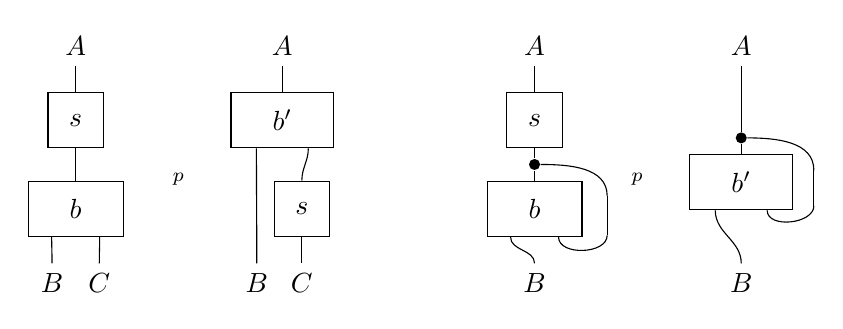
\begin{tikzpicture}
      \node[] (A) at (0, 1.5) {$A$};
      \node[box] (s) at (0, 0.5625) {s};
      \node[box=2/0/2/0] (b) at (0, -0.5625) {\quad b \quad};
      \node[] (B) at (-0.3, -1.5) {$B$};
      \node[] (C) at (0.3, -1.5) {$C$};
      \node[] (r) at (1.3125, -0.225) {$\tref^p$};
      \node[] (A2) at (2.625, 1.5) {$A$};
      \node[box=2/0/2/0] (b2) at (2.625, 0.5625) {\quad b' \quad};
      \node[box] (s2) at (2.8725, -0.5625) {s};
      \node[] (B2) at (2.3, -1.5) {$B$};
      \node[] (C2) at (2.8725, -1.5) {$C$};
      \node[] (r) at (4.35, -0.225) {$\implies$};
      \node[] (A3) at (5.8275, 1.5) {$A$};
      \node[box] (s3) at (5.8275, 0.5625) {s};
      \node[dot] (fix1) at (5.8275, 0) {};
      \coordinate (cap1) at (6.75, -0.4) {};
      \coordinate (cup1) at (6.75, -0.9) {};
      \node[box=2/0/2/0] (b3) at (5.8275, -0.5625) {\quad b \quad};
      \node[] (B3) at (5.8275, -1.5) {$B$};
      \node[] (r2) at (7.14, -0.225) {$\tref^p$};
      \node[] (A4) at (8.4525, 1.5) {$A$};
      \node[dot] (fix2) at (8.4525, 0.3375) {};
      \coordinate (cap2) at (9.375, -0.075) {};
      \coordinate (cup2) at (9.375, -0.525) {};
      \node[box=2/0/2/0] (b4) at (8.4525, -0.225) {\quad b' \quad};
      \node[] (B4) at (8.4525, -1.5) {$B$};
      \wires{ 
        A = { south = s.north },
        s = { south = b.north },
        b = { south.1 = B.north, south.2 = C.north },
        A2 = { south = b2.north },
        b2 = { south.1 = B2.north, south.2 = s2.north },
        s2 = { south = C2.north },
        A3 = { south = s3.north },
        s3 = { south = fix1.north },
        fix1 = { south = b3.north },
        b3 = { south.1 = B3.north, south.2 = cup1.south },
        cup1 = { north = cap1.south },
        cap1 = { north = fix1.east },
        A4 = { south = fix2.north },
        fix2 = { south = b4.north },
        b4 = { south.1 = B4.north, south.2 = cup2.south },
        cup2 = { north = cap2.south },
        cap2 = { north = fix2.east },
      }{}
    \end{tikzpicture}
  \caption{Control-flow graphs for the uniformity rule in Figure~\ref{fig:iteration-rules}}
  \Description{}
  \label{fig:unif-cfg}
\end{figure}

\section{Semantics}

In this section, we will work towards a categorical semantics for \subiterexp{}, which we will later
prove to be sound and complete w.r.t. the refinement theory in Section~\ref{ssec:refinement-theory}.
More precisely, fixing a category $\mc{C}$, we wish to map types $A$ and contexts $\Gamma^{\mb{q}}$
to objects $\dnt{A}$ and $\dnt{\Gamma^{\mb{q}}}$ respectively, and then take the semantics
$\dnt{\hasty{\Gamma^{\mb{q}}}{\epsilon}{a}{A}}$ of a well-typed term to be a morphism
$\mc{C}(\dnt{\Gamma^{\mb{q}}}, \dnt{A})$.

\subsection{Models of \subiterexp{}}

A good categorical semantics is one in which the semantics of a term is constructed in a
straightforward, compositional manner from the semantics of its subterms. Furthermore, we would like
the equational properties of our term formers to correspond closely to the universal properties of
the categorical structure used to interpret them. Thus, our goal is to pick categorical structures
which correspond  one-to-one to the features of \subiterexp{}. In
particular, we need to find categorical structures to model our three primary structured
control-flow constructs, which are:
\begin{itemize}
  \item \emph{Sequencing} and \emph{binding}, which we will do using the structure of a
  \emph{premonoidal category}
  \item \emph{Branching}, which we will do using \emph{coproducts}
  \item \emph{Iteration}, which we will do using a \emph{Conway operator}
\end{itemize}
To maintain compositionality, we must additionally require that these structures interact properly 
with each other. Hence, we will also require our category to satisfy
\begin{itemize}
  \item \emph{Distributivity}, which ensures the premonoidal and coproduct structures are compatible
  \item \emph{Strength}, which ensures the Conway operator is compatible with the premonoidal
  structure
  \item \emph{(Directed) Uniformity}, which ensures the Conway operator is compatible with our
  effect and refinement systems.
\end{itemize}
Finally, we'll need to model the features of our type theory; particularly:
\begin{itemize}
  \item \emph{Refinement}, which we will do using \emph{poset-enrichment}
  \item \emph{Effects}, which we will do by introducing the new notion of a \emph{substructural
  effectful category}
\end{itemize}

In ordinary categorical semantics, we want syntactic equivalence to
correspond to equality of morphisms: given $\tmeq{\Gamma^{\mb{q}}}{\mc{R}}{a}{b}{A}$,
$\dnt{\hasty{\Gamma^{\mb{q}}}{\epsilon}{a}{A}} = \dnt{\hasty{\Gamma^{\mb{q}}}{\epsilon}{b}{A}}$. 

However, in our calculus, we do not only have a syntactic notion of equivalence, but we also have
the order structure arising from refinement. Since terms correpond to morphisms, this means we need
to be able to compare morphisms according to an order structure interpreting the refinement
relation. Thus, to interpret $\tref$, we generalize from ordinary categories to
\emph{poset-enriched} categories, in which our hom-sets are partially ordered. In particular, we
define:

\begin{definition}[Poset-enriched category]
  A category $\mc{C}$ is \emph{poset-enriched} if each hom-set $\mc{C}(A, B)$ is equipped with a
  partial order $\cref$ which is compatible with composition, i.e., which satisfies
  $$
  \forall f \cref f' \in \mc{C}(A, B) . \forall g \tref g' \in \mc{C}(B, C) . 
    (f ; g) \tref (f' ; g')
  $$
  A poset-enriched functor between categories $\mc{C}$, $\mc{D}$ is then simply a functor whose
  action on morphisms is monotonic.
\end{definition}

We can now quite naturally intepret soundness of refinement as follows: given
$\tmle{\Gamma^{\mb{q}}}{\mc{R}}{a}{b}{A}$, we require that
$\dnt{\hasty{\Gamma^{\mb{q}}}{\epsilon}{a}{A}} \cref \dnt{\hasty{\Gamma^{\mb{q}}}{\epsilon}{b}{A}}$.
Soundness of equivalence follows directly from antisymmetry of partial orders.\footnote{Requiring
$\mc{C}$ to be a poset-enriched category does not in fact rob us of any generality, since \emph{all}
categories are poset-enriched under the identity ordering on hom-sets.}


We can now proceed to give poset-enriched versions of the models for our three control-flow
primitives, namely, seqencing, branching, and iteration. Premonoidal categories were introduced in
\citet{power-premonoidal-97} to model side-effectful, sequential computations with first-order
binding. A premonoidal category can be viewed as a generalization of a monoidal category, in which
\emph{sliding} does not necessarily hold; i.e., we have that, in general,
$$
(f \otimes \ms{id}) ; (\ms{id} \otimes g) \neq
(\ms{id} \otimes g) ; (f \otimes \ms{id})
$$
To better understand this in terms of programming languages, a premonoidal
category may also be viewed as a generalization of the Moggi's \cite{moggi-91-monad} monadic
semantics: if we consider a strong monad over a Cartesian category, then the Kleisli category is
premonoidal with the Cartesian product in the underlying category as tensor product. The Kleisli
category satisfies sliding when the underlying monad is
\emph{commutative}: when the sequencing of
side-effects does not matter (e.g., the reader monad). We need to generalize monoidal categories to premonoidal categories
precisely to support monads for which sequencing does matter, such as printing or state. For
example, given a function $\ms{print}: \ms{str} \to ()$,
$$
(\ms{print} \otimes \ms{id}) ; (\ms{id} \otimes \ms{print}) \neq
(\ms{id} \otimes \ms{print}) ; (\ms{print} \otimes \ms{id}) 
$$
and input $(\mathtt{"hello"}, \mathtt{"world"})$, the left-hand side will print $\mathtt{hello
world}$, while the right-hand side will print $\mathtt{world hello}$. Note that the sequencing in
the induced premonoidal category corresponds precisely to the bind of the underlying monad.

We give a precise definition of a premonoidal category, adapted to the poset-enriched setting,
below:
\begin{definition}[Symmetric Premonoidal Category]
  We define a \emph{binoidal category} to be a category $\mc{C}$ equipped with a binary operation
  $\otimes : |\mc{C}| \times |\mc{C}| \to |\mc{C}|$ on the objects of $\mc{C}$ and, for each $A, B
  \in |\mc{C}|$, functors $A \otimes -, - \otimes B : \mc{C} \to \mc{C}$. We say a morphism $f : A
  \to A'$ in a binoidal category is \emph{central} if, for all $g : B \to B'$, it satisfies
  \emph{sliding}:
  $$
  f \otimes B ; A' \otimes g = A \otimes g ; f \otimes B' \qquad
  B \otimes f ; g \otimes A' = g \otimes A ; B' \otimes f
  $$
  in which case we may write these morphisms as $f \otimes g : A \otimes B \to A' \otimes B'$ and $g
  \otimes f : B \otimes A \to B' \otimes A'$ respectively. In the poset-enriched setting, we also
  assume that the left and right tensor functors are poset-enriched, i.e. monotonic on morphisms.
  
  A \emph{premonoidal category} is, then, a
  binoidal category equipped with:
  \begin{itemize}
    \item An \emph{identity} object $I \in |\mc{C}|$
    \item For each triple of objects $A, B, C \in |\mc{C}|$, a central, natural isomorphism
    $\alpha_{A, B, C} : (A \otimes B) \otimes C \to A \otimes (B \otimes C)$, the \emph{associator}
    \item For each object $A$, central, natural isomorphisms $\lambda_A : A \otimes I \to A$ and
    $\rho_A : I \otimes A \to A$, the \emph{left} and \emph{right unitors}
  \end{itemize}
  satisfying the \emph{triangle} and \emph{pentagon identity}
  $$
  \alpha_{A, I, B} ; A \otimes \lambda_B = \rho_A \otimes B \qquad
  \alpha_{A \otimes B, C, D} ; \alpha_{A, B, C \otimes D}
  = \alpha_{A, B, C} \otimes D ; \alpha_{A, B \otimes C, D} ; A \otimes \alpha_{A, B, C}
  $$
  We say a premonoidal category is \emph{symmetric} if it is also equipped with a central, natural
  involution $\sigma_{A, B} : A \otimes B \to B \otimes A$, the \textit{symmetry}, satisfying the
  \emph{hexagon identity}
  $$
  \alpha_{A, B, C} ; \sigma_{A, B \otimes C} ; \alpha_{B, C, A}
  = \sigma_{A, B} \otimes C ; \alpha_{B, A, C} ; B \otimes \sigma_{A, C}
  $$
\end{definition}
This gives us a nice alternate characterization of (poset-enriched) monoidal categories as well:
\begin{definition}[(Symmetric) Monoidal Category]
  We say a (symmetric) premonoidal category is \emph{(symmetric) monoidal} if every morphism is
  central.
\end{definition}
One theorem of note about premonoidal categories is \emph{coherence}, which we state as follows:
\begin{theorem}
  For any premonoidal category $\mc{C}$, the subcategory $\mc{C}_\mc{A}$ generated by associators,
  unitors, and their tensor products is an equivalence relation, i.e., for all $A, B :
  |\mc{C}_\mc{A}|$, if $f, g : A \to B$ can be constructed using only identity, composition,
  associators, unitors, and their tensor products, then:
  \begin{enumerate}[label=(\alph*)]
    \item $f = g$
    \item $f, g$ are isomorphisms in $\mc{C}_\mc{A}$
  \end{enumerate}
  \label{thm:monoidal-coherence}
\end{theorem}
We will hence sometimes abuse notation and write $\alpha_B : \mc{C}(A, B)$ or simply $\alpha$ for
the unique morphism in $\mc{C}_\mc{A}$ from $A$ to $B$, where the composition of associators and
unitors is too cumbersome to write out in full. In particular, we note that we always have that
$\alpha: \mc{C}(A, A) := \ms{id}_A$.

We model branching control-flow using the coproduct $A + B$ as a primitive, whose definition is
unchanged in the poset-enriched setting. Given morphisms $f : A \to C$ and $g : B \to C$, their
coproduct $[f, g] : A + B \to C$ quite naturally models a case-statement which executes $f$ given an
$A$ and executes $g$ given a $B$. We can implement a more traditional if-statement as a
case-statement on the object $\mb{2} = I + I$.

Since coproducts induce a monoidal structure on a category, we will also write $\alpha^+_B :
\mc{C}(A, B)$ or simply $\alpha^+$ to denote the unique morphism from $A$ to $B$ with analogy to the
$\alpha$ notation described above. Similarly, we will write $\sigma^+$ to denote the symmetry for
coproducts.

Coproducts on their own, however, cannot interpret variables captured by the branches of a
case-statement. For example, given $x : \mbb{Z}$, $y : \mbb{Z} + \ms{str}$, consider the following
expression:
$$
\caseexpr{y}{y}{\ms{print}(\texttt{"add: "}, x + y)}{y}{\ms{print}(y, x)}
$$
While our input context corresponds to the object $\mbb{Z} \otimes (\mbb{Z} + \ms{str})$, we need to
somehow get to $(\mbb{Z} \otimes \mbb{Z}) + (\mbb{Z} \otimes \ms{str})$ to be able to evaluate our
branches. Categorically, what we require is that our coproduct is \emph{distributive} over our
tensor product; we define a \emph{distributive category} for which this is the case as follows:
\begin{definition}[Distributive Category]
  We say a premonoidal category is \emph{distributive} if:
  \begin{itemize}
    \item It is equipped with chosen coproducts $A + B$ such that the injections $\iota_l, \iota_r$
    are central
    \item The obvious morphism $\delta : (A \otimes B) + (A \otimes C) \to A \otimes (B + C)$ is an
    isomorphism.
  \end{itemize}
\end{definition}

The last control-flow construct we need to model is looping. A loop with input $A$ will either exit
with output $B$ or recurse with a new input $A$. Consequently, since we model branching control-flow
using coproducts, the \emph{body} of a loop will look like a morphism $A \to B + A$. Therefore, a
natural way to model iteration is to posit the existence of a fixpoint operator $(\cdot)^\dagger$
taking morphisms $f: A \to B + A$ to their fixpoints $f^\dagger: A \to B$. $f^\dagger$ being the
fixpoint of the body $f$ means that executing $f^\dagger$ on an input $A$ is the same as executing
$f$ on an input $A$ and,
\begin{itemize}
  \item If we get an output $B$, return it
  \item If we get an output $A$, feed it as an input to $f^\dagger$ and return the resulting $B$
\end{itemize}
Indeed, in a functional language supporting higher-order functions such as ML or Haskell, we might
write \texttt{iterate :: (A -> B + A) -> A -> B} with definition
\begin{center}
  \begin{minipage}{0.85\textwidth}
    \begin{lstlisting}[language=Haskell]
      iterate f a = case f a of { Left b -> b ; Right a' -> iterate f a' }
    \end{lstlisting}
  \end{minipage}
\end{center}
This corresponds exactly to the notion of a \emph{pre-iterative category} given below:
\begin{definition}[Pre-iterative Category]
  Let $\mc{C}$ be a category with chosen coproducts. We say $\mc{C}$ is \emph{pre-iterative} if it
  is equipped with a fixpoint operator $(-)^\dagger : \mc{C}(A, B + A) \to \mc{C}(A, B)$ satisfying
  the loop unrolling equation $f ; [\ms{id}, f^\dagger] = f$
\end{definition}
Our goal is to have our fixpoint operator's properties correspond precisely to drawing a loop in a
control-flow graph, as in the left-hand side of Figure~\ref{fig:fixpoint-string-diagram}, which
corresponds to $f^\dagger$. In particular, we should be able to reconfigure such diagrams up to
isotopy (i.e., moving boxes and wires around without changing connectivity) without changing the
meaning of our program. To be able to do so soundly, we will need to introduce some additional
equations, which correspond to the graphical transformations in
Figure~\ref{fig:elgot-ax-string-diagrams}; a fixpoint satisfying these equations is called a
\emph{Conway iteration operator}, as defined below:
\begin{definition}[Conway Iteration Operator]
  Given a pre-iterative category $\mc{C}$, we say $(-)^\dagger$ is a \emph{Conway iteration
  operator} if it additionally satisfies
  \begin{itemize}
    \item \emph{Naturality:} given $f : A \to B + A$ and $g : B \to C$, we have
      $
      (f;g + \ms{id})^\dagger = f^\dagger;g : A \to C
      $
    \item \emph{Dinaturality:} given morphisms $g : A \to B + C$ and $h : C \to B + A$, we have that
      $
      (g ; [\iota_l, h])^\dagger = g ; [\ms{id}_B, (h ; [\iota_l, g])^\dagger]
      $
    \item \emph{Codiagonal:} given $f : A \to (B + A) + A$, we have
      $
      (f^\dagger)^\dagger = (f;[\ms{id}, \iota_r])^\dagger : A \to B
      $
  \end{itemize}
\end{definition}

\begin{figure}
  \begin{subfigure}{0.5\textwidth}
    \centering
    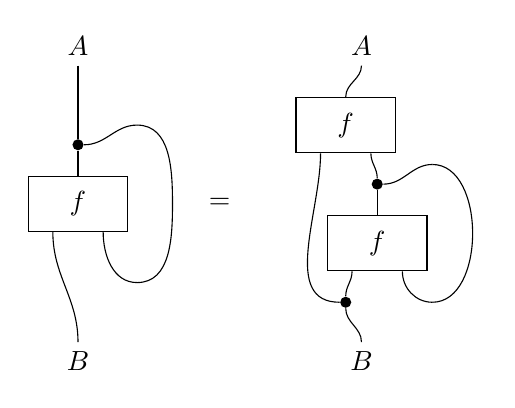
\begin{tikzpicture}
      \node[] (A) at (0, 2) {$A$};
      \node[box=1/0/2/0] (f) at (0, 0) {\quad f \quad};
      \node[] (B) at (0, -2) {$B$};
      \node[dot] (codiag) at (0, 0.75) {};
      \coordinate[] (C) at (1.2, 0) {};
      \coordinate[] (cup) at (0.75, -1) {};
      \coordinate[] (cap) at (0.75, 1) {};
      \node[] (eq) at (1.8, 0) {=};
      \node[] (Ad) at (3.6, 2) {$A$};
      \node[box=1/0/2/0] (fd1) at (3.4, 1) {\quad f \quad};
      \node[dot] (codiagd1) at (3.8, 0.25) {};
      \node[box=1/0/2/0] (fd2) at (3.8, -0.5) {\quad f \quad};
      \node[dot] (codiagd2) at (3.4, -1.25) {};
      \node[] (Bd) at (3.6, -2) {$B$};
      \coordinate[] (cupd) at (4.5, -1.25) {};
      \coordinate[] (capd) at (4.5, 0.5) {};
      \wires{
        A         = { south = codiag.north },
        f         = { south.1 = B, south.2 = cup.west },
        codiag    = { south = f.north, east = cap.west },
        C         = { south = cup.east, north = cap.east },
        Ad        = { south = fd1.north },
        fd1       = { south.1 = codiagd2.west, south.2 = codiagd1.north },
        codiagd1  = { south = fd2.north },
        fd2       = { south.1 = codiagd2.north, south.2 = cupd.west },
        codiagd2  = { south = Bd.north },
        cupd      = { east = capd.east },
        capd      = { west = codiagd1.east }, 
      }{}
    \end{tikzpicture}
    \caption{Fixpoint}
    \label{fig:fixpoint-string-diagram}
  \end{subfigure}%
  \begin{subfigure}{0.5\textwidth}
    \centering
    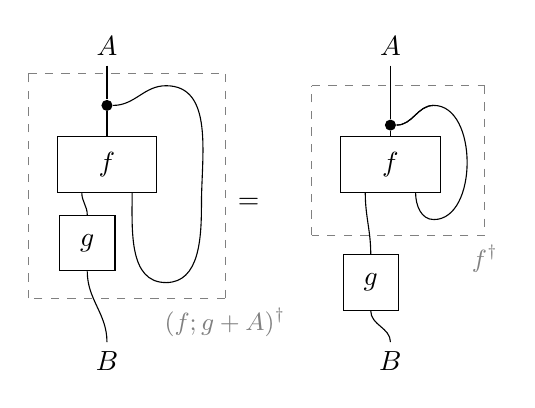
\begin{tikzpicture}
      \node[] (A) at (0, 2) {$A$};
      \node[box=1/0/2/0] (f) at (0, 0.5) {\quad f \quad};
      \node[box] (g) at (-0.25, -0.5) {g};
      \node[] (B) at (0, -2) {$B$};
      \node[dot] (codiag) at (0, 1.25) {};
      \coordinate[] (C) at (1.2, 0) {};
      \coordinate[] (cup) at (0.75, -1) {};
      \coordinate[] (cap) at (0.75, 1.5) {};
      \coordinate[] (box0) at (1.5, 1.65) {};
      \coordinate[label={[font=\small, text=gray]below:$(f;g + A)^\dagger$}] 
                    (box1) at (1.5, -1.2) {};
      \coordinate[] (box2) at (-1, -1.2) {};
      \coordinate[] (box3) at (-1, 1.65) {};
      \draw [gray, dashed] (box0) -- (box1);
      \draw [gray, dashed] (box1) -- (box2);
      \draw [gray, dashed] (box2) -- (box3);
      \draw [gray, dashed] (box3) -- (box0);
      \node[] (eq) at (1.8, 0) {=};
      \node[] (A2) at (3.6, 2) {$A$};
      \node[box=1/0/2/0] (f2) at (3.6, 0.5) {\quad f \quad};
      \node[box] (g2) at (3.35, -1) {g};
      \node[] (B2) at (3.6, -2) {$B$};
      \node[dot] (codiag2) at (3.6, 1) {};
      \coordinate[] (cup2) at (4.15, -0.2) {};
      \coordinate[] (cap2) at (4.15, 1.25) {};
      \coordinate[] (box02) at (4.8, 1.5) {};
      \coordinate[label={[font=\small, text=gray]below:$f^\dagger$}] 
                    (box12) at (4.8, -0.4) {};
      \coordinate[] (box22) at (2.6, -0.4) {};
      \coordinate[] (box32) at (2.6, 1.5) {};
      \draw [gray, dashed] (box02) -- (box12);
      \draw [gray, dashed] (box12) -- (box22);
      \draw [gray, dashed] (box22) -- (box32);
      \draw [gray, dashed] (box32) -- (box02);
      \wires{
        A         = { south = codiag.north },
        f         = { south.1 = g.north, south.2 = cup.west },
        g         = { south = B.north },
        codiag    = { south = f.north, east = cap.west },
        C         = { south = cup.east, north = cap.east },
        A2         = { south = codiag2.north },
        f2         = { south.1 = g2.north, south.2 = cup2.west },
        g2         = { south = B2.north },
        codiag2    = { south = f2.north, east = cap2.west },
        cup2       = { east = cap2.east },
        cap2       = { west = codiag2.east },
      }{}
    \end{tikzpicture}
    \caption{Naturality}
  \end{subfigure}
  \begin{subfigure}{0.5\textwidth}
    \centering
    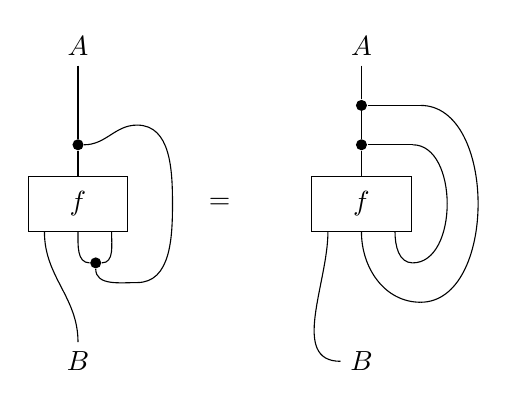
\begin{tikzpicture}
      \node[] (A) at (0, 2) {$A$};
      \node[box=1/0/3/0] (f) at (0, 0) {\quad f \quad};
      \node[] (B) at (0, -2) {$B$};
      \node[dot] (codiag) at (0, 0.75) {};
      \coordinate[] (C) at (1.2, 0) {};
      \coordinate[] (cup) at (0.75, -1) {};
      \coordinate[] (cap) at (0.75, 1) {};
      \node[dot] (codiag2) at (0.225, -0.75) {};
      \node[] (eq) at (1.8, 0) {=};
      \node[] (Ad) at (3.6, 2) {$A$};
      \node[box=1/0/3/0] (fd) at (3.6, 0) {\quad f \quad};
      \node[] (Bd) at (3.6, -2) {$B$};
      \node[dot] (codiagd) at (3.6, 1.25) {};
      \node[dot] (codiagd2) at (3.6, 0.75) {};
      \coordinate[] (Cd) at (4.8, 0) {};
      \coordinate[] (cupd) at (4.35, -1.25) {};
      \coordinate[] (capd) at (4.35, 1.25) {};
      \coordinate[] (cupd2) at (4.25, -0.75) {};
      \coordinate[] (capd2) at (4.25, 0.75) {};
      \wires{
        A         = { south = codiag.north },
        f         = { south.1 = B, south.2 = codiag2.west, south.3 = codiag2.east },
        codiag2   = { south = cup.west },
        codiag    = { south = f.north, east = cap.west },
        C         = { south = cup.east, north = cap.east },
        Ad        = { south = codiagd.north },
        codiagd   = { south = codiagd2.north, east = capd.west },
        codiagd2  = { south = fd.north, east = capd2.west },
        fd        = { south.1 = Bd, south.2 = cupd.west, south.3 = cupd2.west },
        cupd      = { east = capd.east },
        cupd2     = { east = capd2.east },
      }{}
    \end{tikzpicture}
    \caption{Codiagonal}
  \end{subfigure}%
  \begin{subfigure}{0.5\textwidth}
    \centering
    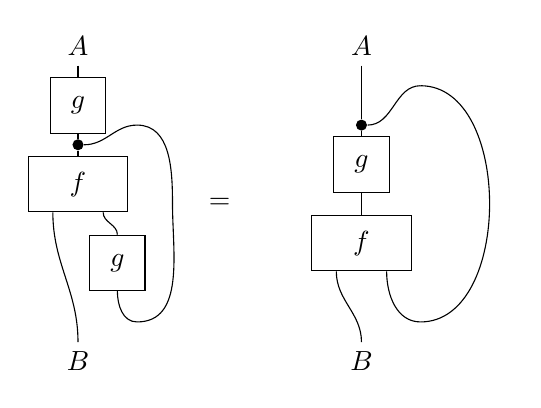
\begin{tikzpicture}
      \node[] (A) at (0, 2) {$A$};
      \node[box] (g) at (0, 1.25) {g};
      \node[box=1/0/2/0] (f) at (0, 0.25) {\quad f \quad};
      \node[] (B) at (0, -2) {$B$};
      \node[dot] (codiag) at (0, 0.75) {};
      \coordinate[] (C) at (1.2, 0) {};
      \coordinate[] (cup) at (0.75, -1.5) {};
      \coordinate[] (cap) at (0.75, 1) {};
      \node[box] (g2) at (0.5, -0.75) {g};
      \node[] (eq) at (1.8, 0) {=};
      \node[] (Ad) at (3.6, 2) {$A$};
      \node[box] (gd) at (3.6, 0.5) {g};
      \node[box=1/0/2/0] (fd) at (3.6, -0.5) {\quad f \quad};
      \node[] (Bd) at (3.6, -2) {$B$};
      \node[dot] (codiagd) at (3.6, 1) {};
      \coordinate[] (Cd) at (4.8, 0) {};
      \coordinate[] (cupd) at (4.35, -1.5) {};
      \coordinate[] (capd) at (4.35, 1.5) {};
      \wires{
        A         = { south = g.north },
        g         = { south = codiag.north },
        f         = { south.1 = B, south.2 = g2.north },
        g2        = { south = cup.west },
        codiag    = { south = f.north, east = cap.west },
        C         = { south = cup.east, north = cap.east },
        Ad        = { south = codiagd.north },
        codiagd   = { south = gd.north, east = capd.west },
        gd        = { south = fd.north },
        fd        = { south.1 = Bd, south.2 = cupd.west },
        cupd      = { east = capd.east },
      }{}
    \end{tikzpicture}
    \caption{Dinaturality}
  \end{subfigure}
  \caption{Representations of the Conway iteration axioms as string diagrams}
  \label{fig:elgot-ax-string-diagrams}
  \Description{Representations of the Conway iteration axioms as string diagrams}
\end{figure}
In particular, we note that naturality and codiagonal correspond directly to our rules
\brle{let-iter} and \brle{codiag} respectively; we will later see that dinaturality is derivable.

Just like for branching control-flow, we also require an additional condition to ensure that our
iteration operator is compatible with our premonoidal structure. Specifically, we would like to be
able to ``thread'' values through our loop bodies; i.e., the following two programs should be
equivalent for \emph{pure} $c$:
$$
(\liter{a}{x}{b}, c) \approx \liter{(a, c)}{(x, y)}
  {\caseexpr{b}{z}{\linl{(z, y)}}{z}{\linr{(z, y)}}}
$$
This corresponds to requiring our Conway iteration operator to be \emph{strong}, defined as follows:
\begin{definition}[Strong Conway Iteration Operator]
  If $\mc{C}$ is distributive, we say an iteration operator $(\cdot)^\dagger$ is \emph{strong} if
  $$
  \forall f: A \to B + A, (C \otimes f ; \delta^{-1})^\dagger = C \otimes f^\dagger
  $$
\end{definition}
We've now got almost everything we need to model pure and arbitrarily effectful \subiterexp{}
programs, but we still need to be able to perform a more fine-grained classification of effects. To
do so, we introduce a generalization of the notion of an \emph{effectful category}, which in the
literature (e.g. \cite{promonad}) only distinguishes between pure and arbitrarily effectful
morphisms.
\begin{definition}[Effectful category]
  An effectful category $\mc{C}$ over an effect system $\mc{E}$ consists of a symmetric premonoidal
  poset-enriched category $\mc{C}$ equipped with a  monotonic mapping from $\epsilon \in \mc{E}$ to
  wide\footnote{A \emph{wide} subcategory is one which has all of the objects of the original
  category.} (symmetric premonoidal) subcategories $\mc{C}_\epsilon \subseteq \mc{E}$ 
  \footnote{
    Note that $\mc{C}_\epsilon(A, B)$ is \emph{not} necessarily closed under refinement:
    we can have $f \in \mc{C}_\epsilon(A, B)$ and $f \cref f'$ with 
    $f' \notin \mc{C}_\epsilon(A, B)$.
  }
  such that,
  given $\epsilon, \eta \in \mc{E}$, $f \in \mc{C}_\epsilon(A, B)$, and $g \in \mc{C}_\eta(A', B')$,
  $\epsilon \rightmove \eta \implies f \ltimes g \cref f \rtimes g$
  and
  $\epsilon \leftmove \eta \implies f \ltimes g \anticref f \rtimes g$.
  We call morphisms with effect $\bot$ \emph{pure}. We say an effectful category is
  \emph{distributive} if the underlying premonoidal category is, and the injections are pure.
\end{definition}
The goal of allowing morphisms with compatible effects to commute is to allow proving substitution
of effectful programs sound. Unfortunately, we don't have quite enough structure to allow
substitution \emph{into} the body of a loop: while commutativity of $a$ and $b$ is enough to justify
that
$
\letexpr{x}{a}{(b, x)} \approx (b, a)
$
proving that
$
\letexpr{x}{a}{\liter{b}{y}{c}} \approx \liter{b}{y}{\letexpr{x}{a}{c}}
$
for $x \notin \ms{fv}(b)$ requires us to be able to move a morphism \emph{into} the body of a loop.
To be able to do that effectively, we need to introduce the concept of a \emph{\mc{K}-uniform
iteration operator} as follows:
\begin{definition}[Uniformity]
  Given a wide subcategory $\mc{K} \subseteq \mc{C}$ of a category equipped with a Conway iteration
  operator, we say $\mc{C}$ is \emph{$\mc{K}^+$-uniform} if, for all $h : A \to_{\mc{K}} B$, $f : B
  \to C + B$, and $g : A \to C + A$, we have that
  $$
  h ; f \cref g ; C + h \implies h ; f^\dagger \cref g^\dagger 
  $$
  and \emph{$\mc{K}^-$-uniform} if
  $$
  h ; f \anticref g ; C + h \implies h ; f^\dagger \anticref g^\dagger 
  $$
  This corresponds precisely to the ability to perform the rewrites shown in
  Figure~\ref{fig:unif-cfg} whenever $s$ is in $\mc{K}$ and $b$ is in $\mc{C}$. We say a category
  $\mc{K}$ is \emph{$\mc{K}$-uniform} if it is both $\mc{K}^+$- and $\mc{K}^-$-uniform, which
  implies in particular that
  $$
  h ; f = g ; C + h \implies h ; f^\dagger = g^\dagger 
  $$
\end{definition}
We briefly note the following useful fact:
\begin{proposition}
  If $(-)^\dagger$ is an iteration operator which satisfies naturality and codiagonal and is
  $\mc{K}$-uniform for $\mc{K}$ cocartesian, then it also satisfies dinaturality.
\end{proposition}
\begin{proof}
  See Lemma 31 of \citet{goncharov-18-guarded-traced}
\end{proof}
Requiring that substitution is compatible with loops is then equivalent to requiring that the
subcategories of morphisms having commutative effects are uniform with respect to each other. We
call this notion an (effectful) Elgot category:
\begin{definition}[Elgot category]
  We say a distributive effectful category $\mc{C}$ is \emph{Elgot} if it has an iterative effect
  system and is equipped with a strong Conway iteration operator, such that, for all effects
  $\epsilon, \eta$ where $\epsilon \in \mc{E}^\infty$,
  \begin{itemize}
    \item The wide subcategory $\mc{C}_\epsilon$ is closed under iteration  
    \item If $\epsilon \rightmove^p \eta$, then $\mc{C}_\epsilon$ is $\mc{C}_\eta^p$-uniform.
  \end{itemize}
  In particular, we note that $\mc{C}$ and hence every $\mc{C}_\epsilon$ is $\mc{C}_\bot$-uniform.
\end{definition}
The final piece of the puzzle is that we need a way to \emph{duplicate} variables of relevant type,
as well as \emph{discard} variables of affine type. We'll supply families of morphisms $\Delta: A
\to A \otimes A$, $!: A \to I$ for this purpose. We can then handle relevant and affine
\emph{effects} by requiring that the appropriate morphism families are \emph{natural} w.r.t. the
subcategory corresponding to that effect. Following this idea, we can now define a \subiterexp-model
as follows: \subiterexp{}:
\begin{definition}[\subiterexp-model]
  A model $\mc{M} = (\mc{C}, (\cdot)^\dagger, \dnt{\cdot}, \dmor{}, \tmor{})$ of a
  \subiterexp-signature $\mc{S} = (\mc{X}, \mc{I}, \mc{E})$ is composed of:
  \begin{itemize}
    \item An effectful Elgot category ($\mc{C}$, $(\cdot)^\dagger$) over $(\mc{E},
    \mc{E}^\infty)$
    \item For each base type $X \in \mc{X}$, an object $\dnt{X} \in |\mc{C}|$, equipped with
    \begin{itemize}
      \item For $X$ affine, a \emph{discard morphism} $\tmor{X} : \mc{C}_\bot(\dnt{X}, I)$
      \item For $X$ relevant, a \emph{diagonal morphism} $\dmor{X} : \mc{C}_\bot(\dnt{X}, \dnt{X}
      \otimes \dnt{X})$
    \end{itemize}
    \item For each function $f : \ms{Inst}(\mc{S})_\epsilon(A, B)$, a morphism $\dnt{f} :
    \mc{C}_\epsilon(\dnt{A}, \dnt{B})$
  \end{itemize}
  such that, for all $A, B \in |\mc{S}|$, $f : \mc{C}_\epsilon(\dnt{A}, \dnt{B})$ we have
  \begin{itemize}
    \item If $A$ relevant, 
      $\dmor{A} ; \dmor{A} \otimes \dnt{A} ; \alpha = \dmor{A} ; \dnt{A} \otimes \dmor{A}$
    \item If $\zeroq \leq \alquant^p(\epsilon)$ and $A, B$ affine, $f ; !_B \cref^p !_A$
    \item If $\zeroq \leq \alquant^p(\epsilon)$ and $A$ relevant, $B$ affine, 
      $\dmor{A} ; (f ; !_B) \otimes \dnt{A} \cref^p \rho^{-1}$
    \item If $\cpyq \leq \alquant^p(\epsilon)$ and $A, B$ relevant, 
    $f ; \dmor{B} \cref^p \dmor{A} ; f \ltimes f = \dmor{A} ; f \rtimes f$
  \end{itemize}
  where
  \begin{itemize}
    \item $\dnt{\mb{1}} = I$, $\dnt{A \otimes B} = \dnt{A} \otimes \dnt{B}$, 
          $!_{\mb{1}} = \ms{id}_I$, and $\Delta_{\mb{1}} = \lambda^{-1} = \rho^{-1}$
    \item For $A, B$ affine, $!_{A \otimes B} = !_A \otimes !_B ; \lambda$, and for $A, B$ relevant, 
    $\Delta_{A \otimes B} 
      = \dmor{A} \otimes \dmor{B}
      ; \sigma^{\ms{mid}}
    $
    where we define
    $
    \sigma^{\ms{mid}}_{A, B, C, D} = 
      \alpha_{A \otimes (B \otimes C) \otimes D}
      ; A \otimes \sigma \otimes D
      ; \alpha
    $
    having type $\mc{C}_\bot(
        (A \otimes B) \otimes (C \otimes D), 
        (A \otimes C) \otimes (B \otimes D)
      )
    $
    \item $\dnt{\mb{0}} = \mb{0}$, $\dnt{A + B} = \dnt{A} + \dnt{B}$, 
          $!_{\mb{0}} = 0_{I}$, and $\Delta_{\mb{0}} = 0_{0 + 0}$
    \item For $A, B$ affine, $!_{A + B} = [!_A, !_B]$, and for $A, B$ relevant, 
    $\Delta_{A + B} 
      = [\dmor{A} ; \iota_l \otimes \iota_l, \dmor{B} ; \iota_r \otimes \iota_r]
    $
  \end{itemize}
\end{definition}
We define the \emph{effective type} of an annotated type $A^q$, $\etoty{A^q}$ to be $\mb{1}$ if
$q = 0$, and $A$ otherwise. We can then proceed to define the effective type of an annotated context
$\Gamma^{\mb{q}}$ to be the tensor product of its variables, i.e., $\etoty{\cdot} = \mb{1}$ and
$\etoty{\Gamma, x : A^q} = \etoty{\Gamma} \otimes \etoty{A^q}$. 
We will abuse notation slightly and extend $\dnt{\cdot}$ to quantity 
annotated types $A^q$ by taking $\dnt{A^q} = \dnt{\etoty{A^q}}$; likewise, we define $!_{A^q} =
!_{\etoty{A^q}}$ and $\Delta_{A^q} = \Delta_{\etoty{A^q}}$, where the \emph{effective type} of an 
annotated type $A^q$, $\etoty{A^q}$, is $\mb{1}$ if $q = 0$, and $A$ otherwise. 
Likewise, we proceed to define the semantics of an annotated context 
$\dnt{\Gamma^{\mb{q}}} : |\mc{C}|$ as $\dnt{\etoty{\Gamma^{\mb{q}}}}$.

We can now define the semantics of our structural judgements, weakenings and context splitting, in
Figure~\ref{fig:struct-sem}. In particular, weakenings simply discard unused variables (which are
guaranteed to be of affine type), while context splitting duplicates variables used in both the left
and right component contexts (which are guaranteed to be of relevant type).

\begin{figure}
  \begin{gather*}
    \boxed{\dnt{\cwk{\Gamma^{\mb{q}}}{\Delta^{\mb{q}'}}} 
      : \mc{C}_\bot(\dnt{\Gamma^{\mb{q}}}, \dnt{\Delta^{\mb{q}'}})} \\
    \dnt{\cwk{\cdot}{\cdot}} = \ms{id}_I \qquad
    \dnt{\cwk{\Gamma^{\mb{q}}, x : A^q_\epsilon}{\Delta^{\mb{q}'}}}
      = \dnt{\Gamma^{\mb{q}}} \otimes !_{A^q}
      ; \lambda
      ; \dnt{\cwk{\Gamma^{\mb{q}}}{\Delta^{\mb{q}'}}} \\
    \dnt{\cwk{\Gamma^{\mb{q}}, x : A^q_\epsilon}
              {\Delta^{\mb{q}'}, x : A^{q'}_{\epsilon'}}}
      = \dnt{\cwk{\Gamma^{\mb{q}}}{\Delta^{\mb{q}'}}} \otimes \begin{cases}
        \ms{id}_{\dnt{A}} & \text{if } q, q' \neq 0 \\
        !_{A^q} & \text{otherwise} \\
      \end{cases}
  \end{gather*}

  \begin{gather*}
    \boxed{\dnt{\qsp{\Gamma}{\mb{q}}{\mb{q}_l}{\mb{q}_r}} 
      : \mc{C}_\bot(\dnt{\Gamma^{\mb{q}}}, 
        \dnt{\Gamma^{\mb{q}_l}_{\mb{e}_l}} \otimes \dnt{\Gamma^{\mb{q}_r}_{\mb{e}_r}})} 
    \\
    \dnt{\qsp{\cdot}{\cdot}{\cdot}{\cdot}} = \rho^{-1}
    \\
    \dnt{\qsp{\Gamma, x : A}{(\mb{q}, q)}{(\mb{q}_l, q_l)}{(\mb{q}_r, q_r)}}
    = \dnt{\qsp{\Gamma}{\mb{q}}{\mb{q}_l}{\mb{q}_r}} \otimes
    \left(\begin{cases}
      \lambda^{-1} & \text{if } q_l = 0 \text{ else} \\
      \rho^{-1} & \text{if } q_r = 0 \text{ else} \\
      \Delta_A & \text{otherwise}
    \end{cases}\right) 
    ; \sigma^{\ms{mid}}
  \end{gather*}
  \caption{Denotational semantics for structural \subiterexp{} judgements}
  \Description{}
  \label{fig:struct-sem}
\end{figure}

\subsection{Semantics of \subiterexp{} Expressions}

We now give the semantics of each of our term formers in Figure~\ref{fig:expr-densem} by induction
on derivations; we write $\dnt{\hasty{\Gamma^{\mb{q}}}{\epsilon}{a}{A}}$ to denote the appropriate
derivation/sub-derivation. Each of them corresponds quite closely to the the underlying categorical
structure. In particular,
\begin{itemize}
  \item We intepret a variable $x$ of type $A$ as the weakening $\cwk{\Gamma^{\mb{q}}}{x : A^1}$;
  this discards all other variables from the input environment.
  \item Let-bindings and pairs are interpreted as sequencing, with, in the former case, the output
  of the first term being passed as an input to the second. In both cases, we use context-splitting
  to apportion the variables between the two terms.
  \item Units are interpreted as the weakening $\cwk{\Gamma^{\mb{q}}}{\cdot}$, i.e., discarding all
  variables.
  \item Case statements are interpreted by passing the result of the discriminator into the
  coproduct of the branches, after context-splitting to apportion the variables between the
  discriminator and branches. We use the distributor to thread the variables into both branches of
  the coproduct, as discussed.
  \item Injections and $\ms{abort}$ are interpreted trivially as the injections and the zero
  morphism respectively, post-composed with their argument.
  \item To interpret iteration, after splitting the context, we interpret the initial value, and
  then feed that into the fixpoint of the body (computed using the Conway iteration operator) along
  with the remainder of the context.
\end{itemize}
We use the $\dnt{\hasty{\Gamma^{\mb{q}}}{\epsilon}{a}{A}}$ notation, rather than specifying a
particular derivation, because \emph{coherence} holds:
\begin{lemma}[Coherence]
  Given derivations $D$ for $\hasty{\Gamma^{\mb{q}}}{\epsilon}{a}{A}$ and $D'$ for
  $\hasty{\Gamma^{\mb{q}}}{\epsilon'}{a}{A}$, we have $\dnt{D} = \dnt{D'}$
\end{lemma}
Observe that the coherence theorem allows us to omit the effect $\epsilon$, because the effect is a
property of the semantics: the same term with two different effect typings will have the same
denotation.

\begin{figure}
  \begin{gather*}
    \boxed{\dnt{\hasty{\Gamma^{\mb{q}}}{\epsilon}{a}{A}} 
      : \mc{C}_\epsilon(\dnt{\Gamma^{\mb{q}}}, \dnt{A})} \\
    \dnt{\hasty{\Gamma^{\mb{q}}}{\epsilon}{x}{A}} 
      = \dnt{\cwk{\Gamma^{\mb{q}}}{x : A^\oneq_\epsilon}}
    \qquad
    \dnt{\hasty{\Gamma^{\mb{q}}}{\epsilon}{f\;a}{B}} 
      = \dnt{\hasty{\Gamma^{\mb{q}}}{\epsilon}{a}{A}} ; \dnt{f} \\
    \dnt{\hasty{\Gamma^{\mb{q}}}{\epsilon}{\letexpr{x}{a}{b}}{B}} 
      = \dnt{\qsp{\Gamma}{\mb{q}}{\mb{q}_l}{\mb{q}_r}}
      ; \dnt{\Gamma^{\mb{q}_l}} 
        \otimes \dnt{\hasty{\Gamma^{\mb{q}_r}}{\epsilon}{a}{A}}
      ; \dnt{\hasty{\Gamma^{\mb{q}_l}, x : A}{\epsilon}{b}{B}}
    \\
    \dnt{\hasty{\Gamma^{\mb{q}}}{\epsilon}{(a, b)}{A \otimes B}}
      = \dnt{\qsp{\Gamma}{\mb{q}}{\mb{q}_l}{\mb{q}_r}}
      ; \dnt{\hasty{\Gamma^{\mb{q}_l}}{\epsilon}{a}{A}}
      \otimes \dnt{\hasty{\Gamma^{\mb{q}_r}}{\epsilon}{b}{B}}
    \\
    \dnt{\hasty{\Gamma^{\mb{q}}}{\epsilon}{()}{\mb{1}}}
      = \dnt{\cwk{\Gamma^{\mb{q}}}{\cdot}}
  \end{gather*}
  \begin{align*}
    \dnt{\hasty{\Gamma^{\mb{q}}}{\epsilon}{\letexpr{(x, y)}{a}{c}}{C}}
    = & \; \dnt{\qsp{\Gamma}{\mb{q}}{\mb{q}_l}{\mb{q}_r}}
      ; \dnt{\Gamma^{\mb{q}_l}}
      \otimes \dnt{\hasty{\Gamma^{\mb{q}_r}}{\epsilon}{a}{A \otimes B}}
    \\ & 
    ; \alpha_{\Gamma^{\mb{q}_r} \otimes A \otimes B}
    ; \dnt{\hasty{\Gamma^{\mb{q}_l}, x : A, y : B}{\epsilon}{c}{C}}
  \end{align*}
  \begin{align*}
    \dnt{\hasty{\Gamma^{\mb{q}}}{\epsilon}{\caseexpr{e}{x}{a}{y}{b}}{C}}
    =& \; 
    \dnt{\qsp{\Gamma}{\mb{q}}{\mb{q}_l}{\mb{q}_r}}
    ; \dnt{\Gamma^{\mb{q}_l}} 
    \otimes \dnt{\hasty{\Gamma^{\mb{q}_r}}{\epsilon}{e}{A + B}}
    ; \delta^{-1} \\ & 
    ; [
      \dnt{\hasty{\Gamma^{\mb{q}_l}, x : A}{\epsilon}{a}{C}},
      \dnt{\hasty{\Gamma^{\mb{q}_l}, y : B}{\epsilon}{b}{C}}
    ]
  \end{align*}
  \begin{gather*}
    \dnt{\hasty{\Gamma^{\mb{q}}}{\epsilon}{\linl{a}}{A + B}}
    = \dnt{\hasty{\Gamma^{\mb{q}}}{\epsilon}{a}{A}} ; \iota_l \qquad
    \dnt{\hasty{\Gamma^{\mb{q}}}{\epsilon}{\linr{b}}{A + B}}
    = \dnt{\hasty{\Gamma^{\mb{q}}}{\epsilon}{b}{B}} ; \iota_r \\
    \dnt{\hasty{\Gamma^{\mb{q}}}{\epsilon}{\labort{a}}{A}}
    = \dnt{\hasty{\Gamma^{\mb{q}}}{\epsilon}{a}{\mb{0}}} ; 0_A
  \end{gather*}
  \begin{align*}
    \dnt{\hasty{\Gamma^{\mb{q}}}{\epsilon}{\liter{a}{x}{b}}{B}}
    &= 
    \dnt{\qsp{\Gamma}{\mb{q}}{\mb{q}_l}{\mb{q}_r}}
    ; \dnt{\Gamma^{\mb{q}_l}}
      \otimes \dnt{\hasty{\Gamma^{\mb{q}_r}}{\epsilon}{a}{A}} \\ &
    ; (
      \dnt{\qsp{\Gamma}{\mb{q}_l}{\mb{q}_l}{\mb{q}_l}} \otimes \dnt{A} 
      ; \alpha
      ; \dnt{\Gamma^{\mb{q}_l}} 
        \otimes \dnt{\hasty{\Gamma^{\mb{q}_r}, x : A}{\epsilon}{b}{B + A}}
      ; \delta^{-1}
    )^\dagger \\ &
    ; \dnt{\cwk{\Gamma^{\mb{q}_l}}{\cdot}} \otimes \dnt{B}
    ; \rho
  \end{align*}
  \caption{Denotational semantics for \subiterexp{} expressions}
  \Description{}
  \label{fig:expr-densem}
\end{figure}

\paragraph{Weakening}

As a sanity check on our semantics, we can verify that it satisfies \emph{weakening} by a
straightforward induction, stated as follows:
\begin{lemma}[Weakening]
  Given $\cwk{\Gamma^{\mb{q}}}{\Delta^{\mb{q}'}}$ and
  $\hasty{\Delta^{\mb{q}'}}{\epsilon}{a}{A}$, we have that
  $$
  \dnt{\cwk{\Gamma^{\mb{q}}}{\Delta^{\mb{q}'}}} ; \dnt{\hasty{\Delta^{\mb{q}'}}{\epsilon}{a}{A}}
  = \dnt{\hasty{\Gamma^{\mb{q}}}{\epsilon}{a}{A}}
  $$
\end{lemma}

\paragraph{Substitution}

We proceed to give a semantics for substitution in Figure~\ref{fig:subst-den}. We split up the input
context into subcontexts for each \emph{used} variable, which are then simply interpreted using
their denotation. Unused variables are simply represented via the left unitor. We can then state
soundness of substitution in the following manner, which is standard except that we prove an
\emph{inequality} whose direction is determined by the commutativity of the effects of the term and
of the substitution. 

\begin{figure}
  \begin{gather*}
    \boxed{\dnt{\issubst{\Gamma^{\mb{q}}}{\epsilon}{\sigma}{\Delta^{\mb{q}'}}}
      : \mc{C}_\epsilon(\dnt{\Gamma^{\mb{q}}}, \dnt{\Delta^{\mb{q}'}})} \\
    \dnt{\issubst{\cdot}{\epsilon}{\cdot}{\cdot}} = \ms{id}_I
    \\
    \dnt{\issubst{\Gamma^{\mb{q}}}{\epsilon}{\sigma, x \mapsto a}{\Delta^{\mb{q}'}, x : A^q}}
    = \begin{cases}
      \dnt{\qsp{\Gamma}{\mb{q}}{\mb{q}_l}{\mb{q}_r}} 
      ; \dnt{\issubst{\Gamma^{\mb{q}_l}_{\mb{e}_l}}{\epsilon}{\sigma}{\Delta^{\mb{q}'}}}
      \otimes \dnt{\hasty{\Gamma^{\mb{q}_r}}{\epsilon}{a}{A}}
      \text{ if } q \neq 0 \\
      \dnt{\issubst{\Gamma^{\mb{q}}}{\epsilon}{\sigma}{\Delta^{\mb{q}'}}}
      ; \lambda^{-1} \text{ otherwise}
    \end{cases}
  \end{gather*}
  \caption{Semantics of \subiterexp{} substitutions}
  \Description{}
  \label{fig:subst-den}
\end{figure}

\begin{theorem}[Soundness of Substitution]
  Given $\issubst{\Gamma^{\mb{q}}}{\eta}{\sigma}{\Delta^{\mb{q'}}}$ and
  $\hasty{\Delta^{\mb{q}'}}{\epsilon}{a}{A}$, we have
  \begin{align*}
  \eta \rightmove \epsilon \implies
  \dnt{\issubst{\Gamma^{\mb{q}}}{\eta}{\sigma}{\Delta^{\mb{q'}}}} 
    ; \dnt{\hasty{\Delta^{\mb{q}'}}{\epsilon}{a}{A}}
  \cref \dnt{\hasty{\Gamma^{\mb{q}}}{}{[\sigma]a}{A}} \\
  \eta \leftmove \epsilon \implies
  \dnt{\issubst{\Gamma^{\mb{q}}}{\eta}{\sigma}{\Delta^{\mb{q'}}}} 
    ; \dnt{\hasty{\Delta^{\mb{q}'}}{\epsilon}{a}{A}}
  \geq \dnt{\hasty{\Gamma^{\mb{q}}}{}{[\sigma]a}{A}}
  \end{align*}
\end{theorem}

\paragraph{Soundness}

Now that we have given our terms a denotational semantics, we would like to show that our refinement
theory is \emph{sound} w.r.t. this semantics. In particular, as we allow a refinement theory to be
parametrized by set of base refinements $\mc{R}$, we need to be able to express whether a model
$\mc{M}$ satisfies these refinements. To do so, we introduce the notion of a model \emph{validating}
a typed refinement family as follows:
\begin{definition}
  We say a model $\mc{M}$ \emph{validates} a typed refinement family $\mc{R}$, written $\mc{M}
  \models \mc{R}$, if, for all
  $
  (\tmle{\Gamma^{\mb{q}}}{}{a}{b}{A}) \in \mc{R}
  $
  we have that
  $
  \dnt{\hasty{\Gamma}{\epsilon}{a}{A}} \tref \dnt{\hasty{\Gamma}{\epsilon}{b}{A}}
  $
\end{definition}
We note that, for every model $\mc{M}$, $\mc{M} \models \varnothing$. We can then phrase soundness
as follows: if $\mc{M}$ models $\mc{R}$, for every refinement in the \emph{theory} generated by
$\mc{R}$, $\ms{Th}(\mc{R})$, $\mc{M}$ validates that refinement. Or, more formally,
\begin{theorem}[Soundness]
  We have that $\mc{M} \models \mc{R} \iff \mc{M} \models \ms{Th}(\mc{R})$. That is, given $\mc{M}
  \models \mc{R}$ and $\tmle{\Gamma^{\mb{q}}}{\mc{R}}{a}{b}{A}$, we have
  $\dnt{\hasty{\Gamma}{\epsilon}{a}{A}}_{\mc{M}} \cref
  \dnt{\hasty{\Gamma}{\epsilon}{b}{A}}_{\mc{M}}$.
\end{theorem}
In particular, we hence have that, for every model $\mc{M}$, $\mc{M} \models \ms{Th}(\varnothing)$,
validating our equational theory.

\paragraph{Syntactic Models and Completeness}

We now wish to show that our equational theory is \emph{complete} with respect to our denotational
semantics; that is, if some refinement holds for every $\mc{M} \models \mc{R}$, then this refinement
is in fact contained in $\ms{Th}(\mc{R})$. We will do this by constructing an \emph{initial} model
$\ms{Tm}(\mc{R})$, the \emph{syntactic model}, such that the following theorem holds:
\begin{theorem}[Completeness]
  If $\dnt{\hasty{\Gamma}{}{a}{A}}_{\ms{Tm}(\mc{R})} \tref
  \dnt{\hasty{\Gamma}{}{b}{A}}_{\ms{Tm}(\mc{R})}$, then
  $
  \tmle{\Gamma}{\mc{R}}{a}{b}{A}
  $
\end{theorem}
It then follows from soundness and the existence of $\ms{Tm}(\mc{R})$ that
$\tmle{\Gamma}{\mc{R}}{a}{b}{A}$ \emph{if and only if} for all models $\mc{M} \models \mc{R}$,
$\dnt{\hasty{\Gamma}{}{a}{A}}_{\mc{M}} \tref \dnt{\hasty{\Gamma}{}{b}{A}}_{\mc{M}}$, as desired.

We now proceed to give a sketch of the construction of $\ms{Tm}(\mc{R})$ and the proof of 
completeness; full details are given in Appendix~\ref{apx:completeness}. As is standard, our 
syntactic model $\ms{Tm}(\mc{R})$ will have types as objects. 
% TODO: rewrite to be purely functional?
To construct morphisms, we start with terms with a single free variable. We stratify these terms by
type and effect as follows:
$$
\ms{Term}(\mc{R})_\epsilon(A, B) := \{(x, a) \mid \hasty{x : A^\top}{\epsilon}{a}{B}\}
$$
We will quotient each $\ms{Term}_\epsilon(\mc{R})$ by term equivalence $\approx_{\mc{R}}$, as well
as by renaming the free variable $x$, to define $\ms{Tm}(\mc{R})_\epsilon$; we will somewhat
suggestively write quotiented pairs $(x, a)$ as lambda-expressions $\lambda x. a$, with $(\lambda x
. a)(y) = [y/x]a$ yielding a term up to equivalence. The identity morphism is simply given as
$\ms{id}_A = (\lambda x. x)$, while composition is given not by substitution (since terms may be
impure!) but rather by let-bindings as follows:
$$
(\lambda x . a) ; (\lambda y . b) := (\lambda x . \letexpr{y}{a}{b})
$$
We can equip $\ms{Tm}(\mc{R})$ with the structure of a poset-enriched category by using the
refinement relation as a partial order; it is trivial to see that this is well-defined. The rest of
the structure of a \subiterexp{}-model is given in Appendix~\ref{apx:syn-model}. To prove
completeness, it then suffices to show that $\dnt{\cdot}_{\ms{Tm}(\mc{R})}$ \emph{reflects}
refinement. The details of how to do so are given in Appendix~\ref{apx:packing}.

% To do so, we note that
% $\dnt{\hasty{\Gamma^{\mb{q}}}{\epsilon}{a}{B}}_{\ms{Tm}(\mc{R})}$ is, up to equivalence, a term of
% the form $\hasty{x : [\Gamma^{\mb{q}}]}{\epsilon}{\bar{a}}{B}$. Hence, our strategy for proving
% completeness is simply to relate the terms $a$ and $\bar{a}$ such that $\bar{a} \tref \bar{b}
% \implies a \tref b$. We begin by relating the contexts $\Gamma^{\mb{q}}$ and $x : [\Gamma^{\mb{q}}]$
% via the \emph{packing lemma}
% \begin{lemma}[name=Packing, restate=packinglemma]
%   We can define monotone functions $\ms{pack}$, $\ms{unpack}_{\Gamma, x}$ on derivations
%   $$
%   \hasty{\Gamma^{\mb{q}}, \Delta^{\mb{q}'}}{\epsilon}{
%         \ms{pack}(\hasty{\Gamma^{\mb{q}}, x : \etoty{\Delta^{\mb{q}'}}}{\epsilon}{a}{A})
%   }{A} \qquad
%   \hasty{\Gamma^{\mb{q}}, x : \etoty{\Delta^{\mb{q}'}}}{\epsilon}{
%         \ms{unpack}_{\Gamma, x}(\hasty{\Gamma^{\mb{q}}, \Delta^{\mb{q}'}}{\epsilon}{b}{A})
%   }{A}
%   $$
%   which are
%   \begin{itemize}
%     \item Semantics-preserving: 
%       \begin{align*}
%       \dnt{\hasty{\Gamma^{\mb{q}}, \Delta^{\mb{q}'}}{\epsilon}{
%         \ms{pack}(\hasty{\Gamma^{\mb{q}}, x : \etoty{\Delta^{\mb{q}'}}}{\epsilon}{a}{A})
%         }{A}}
%         &= \alpha ; \dnt{\hasty{\Gamma^{\mb{q}}, x : \etoty{\Delta^{\mb{q}'}}}{\epsilon}{a}{A}}
%       \\
%       \dnt{\hasty{\Gamma^{\mb{q}}, x : \etoty{\Delta^{\mb{q}'}}}{\epsilon}{
%         \ms{unpack}_{\Gamma, x}(\hasty{\Gamma^{\mb{q}}, \Delta^{\mb{q}'}}{\epsilon}{b}{A})\
%         }{A}}
%         &= \alpha ; \dnt{\hasty{\Gamma^{\mb{q}}}{\epsilon}{b}{A}}
%       \end{align*} 
%     \item Mutually inverse (up to $\approx$):
%         $
%         \tmeq{\Gamma^{\mb{q}}, x : \etoty{\Delta^{\mb{q}'}}}{\mc{R}}
%         {\ms{unpack}_{\Gamma, x}(\ms{pack}(
%           \hasty{\Gamma^{\mb{q}}, x : \etoty{\Delta^{\mb{q}'}}}{\epsilon}{a}{A}
%         ))}
%         {a}
%         {A}
%         $
%         and
%         $
%         \tmeq{\Gamma^{\mb{q}}, \Delta^{\mb{q}'}}{\mc{R}}
%         {\ms{pack}(\ms{unpack}_{\Gamma, x}(
%           \hasty{\Gamma^{\mb{q}, \Delta^{\mb{q}'}}}{\epsilon}{b}{A}))}
%         {b}
%         {A}
%         $
%   \end{itemize}
%   \label{lem:packing}
% \end{lemma}
% We write $\ms{unpack}_x$ as shorthand for $\ms{unpack}_{\cdot, x}$. We may now state the
% \emph{unpacking lemma} as follows: 
% \begin{lemma}[name=Unpacking, restate=unpackinglemma]
%   Given $\hasty{\Gamma^{\mb{q}}}{}{a}{A}$, 
%   for all $(x, \bar{a}) \in \dnt{\hasty{\Gamma^{\mb{q}}}{}{a}{A}}_{\ms{Tm}(\mc{R})}$
%   we have that
%   $
%     \tmeq{\Gamma^{\mb{q}}}{\mc{R}}
%       {\ms{unpack}_{\cdot, \Gamma}(\hasty{x : [\Gamma^{\mb{q}}])}{}{\bar{a}}{A}}
%       {a}{A}
%   $
%   \label{lem:unpacking}
% \end{lemma}
% Completeness follows directly, since, in this case, by monotonicity, for all $(x, \bar{a}) \tref (y,
% \bar{b})$, we have that
% $
% \tmle{\Gamma^{\mb{q}}}{\mc{R}}
%   {\ms{unpack}_{\cdot, x}(\hasty{x : [\Gamma^{\mb{q}}])}{}{\bar{a}}{A}}
%   {\ms{unpack}_{\cdot, y}(\hasty{y : [\Gamma^{\mb{q}}])}{}{\bar{b}}{A}}{A}
% $
% and hence that 
% $
% a \tref b
% $
% as desired. Details of the definition of $\ms{pack}$ and $\ms{unpack}$ and the proofs of
% Lemmas~\ref{lem:packing} and \ref{lem:unpacking} are given in Appendix~\ref{apx:packing}.

\section{SSA Typing and Semantics}

\subsection{Typing Rules}

We now turn back to the promises at the end of Section~\ref{sec:ssa-intro} and attempt to give 
typing rules and denotational semantics for \isotopessa{}. Recall that the primitive syntactic 
element of an \isotopessa{} program is a \emph{region} $r$, which can be viewed as a program 
fragment with a single entry point and multiple exit points. Consequently, our primitive typing 
judgement will be of the form
$$
\boxed{\haslb{\Gamma^{\mb{q}}}{\epsilon}{r}{\ms{L}^{\mb{Q}}}}
$$
which means that
\begin{itemize}
  \item \emph{If} the variables in $\Gamma$ are live on entry, with quantity $\mb{q}$
  \item \emph{Then} executing the region $r$ jumps to one of the labels in $\ms{L}$, with 
  \emph{leftover} quantities $\mb{Q}$.
\end{itemize}
Here, $\ms{L}$ is a list of labels $\ell_i$, annotated with a single parameter type 
(multiple parameters are implemented as a single tuple parameter), and $\mb{Q}$ is a list of 
quantity vectors $\mb{q}_i$ which we call the \emph{quantity matrix}.

We may define a weakening judgement on annotated label contexts using the rules in 
Figure~\ref{fig:label-wk}; the judgement is with respect to a particular context $\Gamma$ used to 
interpret the quantity vectors in $\mb{Q}$. In particular, weakening allows us to  insert arbitrary 
labels using \brle{skip}, as well as weaken the quantities associated with each
using \brle{cons}.
As we can see, a label context is interpreted w.r.t. a quantity matrix $\mb{Q}$, which also depends
on the set of live variables $\Gamma$. To extend the set of live variables 
(e.g. to type a let-binding), we need to zero-pad the quantity matrix, an operation which we call 
\emph{lifting}. This may be defined inductively as follows:
\begin{equation*}
  \zeroqv{\cdot} = \cdot \qquad
  \zeroqv{(\mb{Q}; \mb{q})} = \zeroqv{\mb{Q}} ; (\mb{q}, 0)
\end{equation*} 
It is easy to prove that label weakening is compatible with lifting, i.e. the following rule is 
derivable:
\begin{equation*}
  \prftree[r]{\rle{lift}}
    {\lwk{\Gamma}{\ms{L}^{\mb{Q}}}{\ms{K}^{\mb{Q}'}}}
    {\lwk{\Gamma, x : A}{\ms{L}^{\zeroqv{\mb{Q}}}}{\ms{K}^{\zeroqv{\mb{Q}'}}}}
\end{equation*}

\begin{figure}
  \hspace{4em}
  \begin{subfigure}[t]{.25\textwidth}
  \begin{grammar}
    <\(\ms{L}\)> ::= \(\cdot\) \;|\; \(\ms{L}, \lhyp{\ell}{A}\)
  \end{grammar}
  \end{subfigure}%
  \begin{subfigure}[t]{.25\textwidth}
  \begin{grammar}
    <\(\mb{Q}\)> ::= \(\cdot\) \;|\; \(\mb{Q}; \mb{q}\)
  \end{grammar}
  \end{subfigure}%
  \caption{Grammar for label contexts}
  \Description{}
  \label{fig:label-grammar}
\end{figure}

\begin{figure}
\begin{gather*}
  \prftree[r]{\rle{nil}}{\lwk{\Gamma}{\cdot}{\cdot}} \qquad 
  \prftree[r]{\rle{cons}}
    {\lwk{\Gamma}{\ms{L}^{\mb{Q}}}{\ms{K}^{\mb{Q}}}}
    {\cwk{\Gamma^{\mb{q}'}}{\Gamma^{\mb{q}}}}
    {\lwk{\Gamma}{\ms{L}^{\mb{Q}}, \lhyp{\ell}{A}^{\mb{q}}}
    {\ms{K}^{\mb{Q}}, \lhyp{\ell}{A}^{\mb{q}'}}} \qquad
  \prftree[r]{\rle{skip}}
    {\lwk{\Gamma}{\ms{L}^{\mb{Q}}}{\ms{K}^{\mb{Q}}}}
    {|\Gamma| = |\mb{q}|}
    {\lwk{\Gamma}{\ms{L}^{\mb{Q}}}{\ms{K}^{\mb{Q}}, \lhyp{\ell}{A}^{\mb{q}}}}
\end{gather*}
\caption{Rules for weakening label contexts}
\Description{}
\label{fig:label-wk}
\end{figure}

We now go over the typing rules for \isotopessa{}, given in Figure~\ref{fig:ssa-typing}. We note
that instructions $o$ are simply treated as restricted expressions in \subiterexp{}, and typed 
accordingly.
\begin{itemize}
  \item We begin with the typing rule for branches, \brle{br}. This states that, if $o$ is a pure
  expression of type $A$, and $\ell(A)^{\mb{q}_l}$ weakens to the label context 
  $\ms{L}^{\mb{Q}}$, where $\mb{q}_l$ is the quantities left over after typing $o$, then
  $\brb{\ell}{o}$ is a valid branch into $\ms{L}^{\mb{Q}}$
  \item Let-bindings are typed using \brle{let$_1$} and \brle{let$_2$}, which are exactly the same
  as the corresponding rule for expressions, except that we target a label-context, which needs to
  be lifted (i.e. $\mb{Q}$ replaced with $\zeroqv{\mb{Q}}$) in the premise to deal with the 
  additional variable in the input context.
  \item Case terminators are typed using \brle{case}, which is again the same as the rule for 
  expressions modulo lifting, except for the fact that the discriminator $o$ is required to be
  pure.
  \item \ms{where}-blocks are typed using \brle{where$_\ms{nonrec}$} and \brle{where$_\ms{rec}$}, 
  which we distinguish since the effect of an \ms{where_{rec}} subtree must be iterative 
  (since, for example, we often track potential nontermination as an explicit effect).

  \brle{where$_\ms{nonrec}$} subtrees are composed of an entry subtree $\kappa$, which we take to target
  the compound label-context $\ms{L}^{\mb{Q}}, \ms{R}^{\mb{Q}'}$, and,
  for each \emph{sublabel} in $\ell_i(A_i)^{\mb{q_i}}$ in $\ms{R}^{\mb{Q}'}$, an 
  associated \emph{subregion} $t_i$ which, with variables $\Gamma^{\mb{q}_i}$ plus an argument 
  $x_i : A_i$ live on entry, targets the exit labels $\ms{L}^{\mb{Q}}$. 
  This is non-recursive since the $\ms{R}^{\mb{Q}'}$ cannot call themselves, but we can 
  encode any DAG since the inner subtree $\kappa$ can contain other regions.

  \brle{where$_\ms{rec}$} simply requires the effect $\epsilon$ to be iterative, and in exchange 
  allows the $t_i$ to make recursive calls to sublabels in $\ms{R}^{\mb{Q}'}$.
\end{itemize}

\begin{figure}
  \begin{gather*}
    \prftree[r]{\rle{br}}
      {\qsp{\Gamma}{\mb{q}}{\mb{q}_l}{\mb{q}_r}}
      {\hasty{\Gamma^{\mb{q}_r}}{\bot}{o}{A}}
      {\lwk{\Gamma}{\lhyp{\ell}{A}^{\mb{q}_l}}{\ms{L}^{\mb{Q}}}}
      {\haslb{\Gamma^{\mb{q}}}{\epsilon}{\brb{\ell}{o}}{\ms{L}^{\mb{Q}}}}
    \\
    \prftree[r]{\rle{let$_1$}}
      {\qsp{\Gamma}{\mb{q}}{\mb{q}_l}{\mb{q}_r}}
      {\hasty{\Gamma^{\mb{q}_r}}{\epsilon}{o}{A}}
      {\haslb{\Gamma^{\mb{q}_l}, x : A}{\epsilon}{t}{\ms{L}^{\zeroqv{\mb{Q}}}}}
      {\haslb{\Gamma^{\mb{q}}}{\epsilon}{\letstmt{x}{o}{t}}{\ms{L}^{\mb{Q}}}}
    \\
    \prftree[r]{\rle{let$_2$}}
      {\qsp{\Gamma}{\mb{q}}{\mb{q}_l}{\mb{q}_r}}
      {\hasty{\Gamma^{\mb{q}_r}}{\epsilon}{o}{A \otimes B}}
      {\haslb{\Gamma^{\mb{q}_l}, x : A, y : B}{\epsilon}{t}
        {\ms{L}^{\zeroqv{(\zeroqv{\mb{Q}})}}}}
      {\haslb{\Gamma^{\mb{q}}}{\epsilon}{\letstmt{(x, y)}{o}{t}}{\ms{L}^{\mb{Q}}}}
    \\
    \prftree[r]{\rle{case}}
      {\qsp{\Gamma}{\mb{q}}{\mb{q}_l}{\mb{q}_r}}
      {\hasty{\Gamma^{\mb{q}_r}}{\bot}{o}{A + B}}
      {\haslb{\Gamma^{\mb{q}_l}, x : A}{\epsilon}{\tau_l}
        {\ms{L}^{\zeroqv{\mb{Q}}}}}
      {\haslb{\Gamma^{\mb{q}_l}, y : B}{\epsilon}{\tau_r}
        {\ms{L}^{\zeroqv{\mb{Q}}}}}
      {\haslb{\Gamma^{\mb{q}}}{\epsilon}{\casestmt{o}{x}{\tau_l}{y}{\tau_r}}
                                                {\ms{L}^{\mb{Q}}}}
    \\
    \prftree[r]{\rle{where$_{\ms{nonrec}}$}}
      {\haslb{\Gamma^{\mb{q}}}{\epsilon}{\kappa}
        {\ms{L}^{\mb{Q}}, \ms{R}^{\mb{Q}'}}}
      {\forall \lhyp{\ell_i}{A_i}^{\mb{q}_i} \in \ms{R}^{\mb{Q}'} .
        \haslb{\Gamma^{\mb{q}_i}, x_i : A_i}{\epsilon}{t_i}{\ms{L}^{\zeroqv{\mb{Q}}}}
      }
      {\haslb{\Gamma^{\mb{q}}}{\epsilon}{\awhere{\kappa}{(\wbranch{\ell_i}{x_i}{t_i},)_i}}
        {\ms{L}^{\mb{Q}}}}
    \\
    \prftree[r]{\rle{where$_{\ms{rec}}$}}
    {\haslb{\Gamma^{\mb{q}}}{\epsilon}{\kappa}
      {\ms{L}^{\mb{Q}}, \ms{R}^{\mb{Q}'}}}
    {\einf{\epsilon}}
    {\forall \lhyp{\ell_i}{A_i}^{\mb{q}_i} \in \ms{R}^{\mb{Q}'} .
      \haslb{\Gamma^{\mb{q}_i}, x_i : A_i}{\epsilon}{t_i}{
        \ms{L}^{\zeroqv{\mb{Q}}}, \ms{R}^{\zeroqv{\mb{Q}'}}}
    }
    {\haslb{\Gamma^{\mb{q}}}{\epsilon}{\cwhere{\kappa}{(\wbranch{\ell_i}{x_i}{t_i},)_i}}
      {\ms{L}^{\mb{Q}}}}
  \end{gather*}
  \caption{Typing rules for \isotopessa{}}
  \Description{}
  \label{fig:ssa-typing}
\end{figure}

\subsection{Denotational Semantics}

We can now proceed to give a denotational semantics for \isotopessa{}, which targets an arbitrary
\subiterexp{} model of our signature. We'd like to interpret a judgement 
$\haslb{\Gamma^{\mb{q}}}{\epsilon}{r}{\ms{L}^{\mb{Q}}}$ as a morphism from the input state, 
the set of live variables $\dnt{\Gamma^{\mb{q}}}$, to the output state, which consists of a label 
$\ell_i$ in $\ms{L}$, its argument $A_i$, and leftover variables $\mb{q}_i$ in $\mb{Q}$. To 
represent this as a type, we can defint the (context-dependent) \emph{effective type} of an
annotated label context as follows:
\begin{equation*}
  \ltoty{\Gamma}{\cdot} = \mb{0} \qquad
  \ltoty{\Gamma}{\ms{L}^{\mb{Q}}, \ell(A)^{\mb{q}}} 
    = \ltoty{\Gamma}{\ms{L}^{\mb{Q}}} + \etoty{\Gamma^{\mb{q}}} \otimes A
\end{equation*}
Here, the label is encoded as the branch of the coproduct we end up in, with each branch carrying
the argument and any leftover variables as data. We may now give a denotational semantics for label 
contexts and label weakenings in Figure~\ref{fig:lwk-densem}. 
It is easy to verify that we can reassociate 
$
\alpha^+ : \mc{C}_\bot(
  \dnt{\ms{L}^{\mb{Q}}, \ms{R}^{\mb{Q}'}}(\Gamma),
  \dnt{\ms{L}^{\mb{Q}}}(\Gamma) + \dnt{\ms{R}^{\mb{Q}'}}(\Gamma)
)
$.
We also note that we can apply the 
associator ``pointwise'' to reassociate
$\alpha^\downarrow: \mc{C}_\bot(
  \dnt{\ltoty{\Gamma, x : A}{\ms{L}^{\zeroqv{\mb{Q}}}}}, 
  \dnt{\ltoty{\Gamma}{\ms{L}^{\mb{Q}}}}
)$; 
we will use this freely in our semantics. 

We can now give our semantics for regions in Figure~\ref{fig:ssa-densem}; just like for the typing
judgements, the semantics of operations is given by the semantics of the corresponding \subiterexp{}
expressions.
\begin{itemize}
  \item Branches are interpreted by splitting the context, evaluating the argument expression,
  and then passing the remainder of the context and the evaluated argument into the appropriate
  label weakening.
  \item The denotation of let- and case-statements is exactly the same as for expressions,
  except that we need to re-associate the output object from 
  $\dnt{\ms{L}^{\zeroqv{Q}}}(\Gamma, -)$ to $\dnt{\ms{L}^{\mb{Q}}}$.
  \item The denotation of non-recursive \ms{where}-subtrees is given by the denotation of their
  entry subtree, reassociated to the sum of the exit labels $\ms{L}^{\mb{Q}}$ and sublabels 
  $\ms{R}^{\mb{Q}'}$. The exit labels are then passed through as is, while the sublabels $\ell_i$ 
  are passed to the denotation of the appropriate subregion $t_i$.
  \item The denotation of a recursive \ms{where}-subtree is the same as above, except, since each
  subregion targets $\ms{L}^{\mb{Q}}, \ms{R}^{\mb{Q}'}$, we take the \emph{fixpoint} of the sum
  of the denotations of the subregions viewed as morphisms from $\dnt{\ms{R}^{\mb{Q}}}(\Gamma)$
  to $\dnt{\ms{L}^{\mb{Q}}}(\Gamma) + \dnt{\ms{R}^{\mb{Q}}}(\Gamma)$, i.e., mapping any recursive
  calls back into the body of the where-block.
\end{itemize}

\begin{figure}
  \begin{gather*}
    \boxed{\dnt{\lwk{\Gamma}{\ms{L}^{\mb{Q}}}{\ms{K}^{\mb{Q}'}}} 
      : \mc{C}_\bot(\dnt{\ltoty{\Gamma}{\ms{L}^{\mb{Q}}}}, 
                    \dnt{\ltoty{\Gamma}{\ms{K}^{\mb{Q}'}}})} \\
    \dnt{\lwk{\Gamma}{\cdot}{\cdot}} = \ms{id}_{\mb{0}} \qquad
    \dnt
      {\lwk{\Gamma}{\ms{L}^{\mb{Q}}, \lhyp{\ell}{A}^{\mb{q}}}
      {\ms{K}^{\mb{Q}'}, \lhyp{\ell}{A}^{\mb{q}'}}}
    = \dnt{\lwk{\Gamma}{\ms{L}^{\mb{Q}}}{\ms{K}^{\mb{Q}'}}} 
      + \dnt{\cwk{\Gamma^{\mb{q}}}{\Gamma^{\mb{q}'}}} \otimes \dnt{A} \\
    \dnt
      {\lwk{\Gamma}{\ms{L}^{\mb{Q}}}
      {\ms{K}^{\mb{Q}'}, \lhyp{\ell}{A}^{\mb{q}}}}
    = \dnt{\lwk{\Gamma}{\ms{L}^{\mb{Q}}}{\ms{K}^{\mb{Q}'}}} ; \iota_l
  \end{gather*}
  \caption{Denotational semantics for label contexts and label weakenings}
  \Description{}
  \label{fig:lwk-densem}
\end{figure}

\begin{figure}
  \begin{gather*}
    \boxed{\dnt{\haslb{\Gamma}{\epsilon}{t}{\ms{L}^{\mb{Q}}}}
    : \mc{C}_\epsilon(\dnt{\Gamma^{\mb{q}}}, \ltoty{\Gamma}{\dnt{\ms{L}^{\mb{Q}}}})} \\
    \dnt
    {\haslb{\Gamma^{\mb{q}}}{\epsilon}{\brb{\ell}{a}}{\ms{L}^{\mb{Q}}}}
    = \dnt{\qsp{\Gamma}{\mb{q}}{\mb{q}_l}{\mb{q}_r}}
    ; - \otimes \dnt{\hasty{\Gamma^{\mb{q}_r}}{\bot}{a}{A}}
    ; \iota_r
    ; \dnt{\lwk{\Gamma}{\lhyp{\ell}{A}^{\mb{q}_l}}{\ms{L}^{\mb{Q}}}}
    \\
    \dnt
    {\haslb{\Gamma^{\mb{q}}}{\epsilon}{\letstmt{x}{o}{t}}{\ms{L}^{\mb{Q}}}}
    =
    \dnt{\qsp{\Gamma}{\mb{q}}{\mb{q}_l}{\mb{q}_r}}
    ; - \otimes \dnt{\hasty{\Gamma^{\mb{q}_r}}{\epsilon}{o}{A}}
    ; \dnt{\hasty{\Gamma^{\mb{q}_l}, x : A}{\epsilon}{t}{\ms{L}^{\zeroqv{\mb{Q}}}}}
    ; \alpha^\downarrow \\
    \dnt
    {\haslb{\Gamma^{\mb{q}}}{\epsilon}{\letstmt{(x, y)}{o}{t}}{\ms{L}^{\mb{Q}}}}
    =
    \dnt{\qsp{\Gamma}{\mb{q}}{\mb{q}_l}{\mb{q}_r}}
    ; - \otimes \dnt{\hasty{\Gamma^{\mb{q}_r}}{\epsilon}{o}{A \otimes B}}
    ; \alpha
    \\
    \qquad 
    ; \dnt{\hasty{\Gamma^{\mb{q}_l}, x : A, y : B}{\epsilon}{t}
      {\ms{L}^{\zeroqv{(\zeroqv{\mb{Q}})}}}}
    ; \alpha^\downarrow ; \alpha^\downarrow
    \\
    \dnt
    {\haslb{\Gamma^{\mb{q}}}{\epsilon}{\casestmt{o}{x}{\tau_l}{y}{\tau_r}}
      {\ms{L}^{\mb{Q}}}}
    = \dnt{\qsp{\Gamma}{\mb{q}}{\mb{q}_l}{\mb{q}_r}}
    ; - \otimes \dnt{\hasty{\Gamma^{\mb{q}_r}}{\bot}{o}{A + B}}
    ; \delta^{-1}
    \\
    \qquad
    ; [
      \dnt{\hasty{\Gamma^{\mb{q}_l}, x : A}{\epsilon}{\tau_l}{\ms{L}^{\zeroqv{\mb{Q}}}}}
        ; \alpha^\downarrow,
      \dnt{\hasty{\Gamma^{\mb{q}_l}, y : B}{\epsilon}{\tau_r}{\ms{L}^{\zeroqv{\mb{Q}}}}}
        ; \alpha^\downarrow
    ]
    \\
    \dnt
    {\haslb{\Gamma^{\mb{q}}}{\epsilon}{\awhere{\kappa}{(\wbranch{\ell_i}{x_i}{t_i},)_i}}
      {\ms{L}^{\mb{Q}}}}
    =
    \dnt{\haslb{\Gamma^{\mb{q}}}{\epsilon}{\kappa}
      {\ms{L}^{\mb{Q}}, \ms{R}^{\mb{Q}'}}}
    \\ 
    \qquad ; [
      \ms{id}_{\dnt{\ltoty{\Gamma}{\ms{L}^{\mb{Q}}}}},
      [
        \dnt{\hasty{\Gamma^{\mb{q}_i}, x_i : A_i}{\epsilon}{t_i}
          {\ms{L}^{\zeroqv{\mb{Q}}}}} ; \alpha^\downarrow,
      ]_{\ell_i(A_i)^{\mb{q}_i} \in \ms{R}^{\mb{Q}'}}
    ]
    \\
    \dnt
    {\haslb{\Gamma^{\mb{q}}}{\epsilon}{\cwhere{\kappa}{(\wbranch{\ell_i}{x_i}{t_i},)_i}}
      {\ms{L}^{\mb{Q}}}}
    = \dnt{\haslb{\Gamma^{\mb{q}}}{\epsilon}{\kappa}
      {\ms{L}^{\mb{Q}}, \ms{R}^{\mb{Q}'}}}
    \\
    \qquad ; [
      \ms{id}_{\dnt{\ltoty{\Gamma}{\ms{L}^{\mb{Q}}}}},
      [
        \dnt{\hasty{\Gamma^{\mb{q}_i}, x_i : A_i}{\epsilon}{t_i}
          {\ms{L}^{\zeroqv{\mb{Q}}}, \ms{R}^{\zeroqv{\mb{Q}'}}}} ; \alpha^\downarrow ; \alpha^+,
      ]_{\ell_i(A_i)^{\mb{q}_i} \in \ms{R}^{\mb{Q}'}}^\dagger
    ]
  \end{gather*}
  \caption{Denotational semantics for \isotopessa{}}
  \Description{}
  \label{fig:ssa-densem}
\end{figure}

\subsection{Interconversion with \subiterexp{}}

% Given a rewrite system $\mc{R}$, we say an \isotopessa{} region 
% $\haslb{\Gamma^{\mb{q}}}{\epsilon}{r}{\ms{L}^{\mb{Q}}}$ is refined by $r'$, written
% $\lbref{\Gamma^{\mb{q}}}{\mc{R}}{r}{r'}{\ms{L}^{\mb{Q}}}$ if, 
% for all  models $\mc{M} \models \mc{R}$, we have
% $
% \dnt{\haslb{\Gamma^{\mb{q}}}{\epsilon}{r}{\ms{L}^{\mb{Q}}}}_{\mc{M}} 
% \tref \dnt{\haslb{\Gamma^{\mb{q}}}{\epsilon}{r'}{\ms{L}^{\mb{Q}}}}_{\mc{M}}
% $; in particular, two programs are \emph{equivalent} if their semantics are always equal.

When we say that \isotopessa{} and \subiterexp{} are \emph{equivalent}, what we mean is that there
are \emph{semantics-preserving} functions $\ms{SSA}$, $\ms{Expr}$ on derivations satisfying
\begin{align*}
\dnt{
  \haslb{\Gamma^{\mb{q}}}{\epsilon}{\ms{SSA}_\ell(\hasty{\Gamma^{\mb{q}}}{\epsilon}{a}{A})}
  {\ell(A)^0}
}_{\mc{M}} &= \dnt{\hasty{\Gamma^{\mb{q}}}{\epsilon}{a}{A}}_{\mc{M}} ; \alpha^+ \\
\dnt{
  \hasty{\Gamma^{\mb{q}}}{\epsilon}
    {\ms{Expr}(\haslb{\Gamma^{\mb{q}}}{\epsilon}{r}{\ms{L}^{\mb{Q}}})}
    {\ltoty{\Gamma}{\ms{L}^{\mb{Q}}}}
}_{\mc{M}} &= \dnt{\haslb{\Gamma^{\mb{q}}}{\epsilon}{r}{\ms{L}^{\mb{Q}}}}_{\mc{M}}
\end{align*}
for arbitrary models $\mc{M}$. \footnote{
  The astute reader will note that these functions are not 
  \emph{quite} mutually inverse, since the output of a round-trip 
  $\ms{SSA}(\ms{Expr}(\haslb{\Gamma^{\mb{q}}}{\epsilon}{r}{\ms{L}^{\mb{Q}}}))$ now targets a 
  \emph{single} label with an argument of type $\ltoty{\Gamma}{\ms{L}^{\mb{Q}}}$. This is a somewhat
  thorny problem since the leftover variables in $\mb{Q}$ can be unpacked using an $\ms{L}$-ary 
  case-statement, but cannot \emph{escape} that case-statement. We can't get around this problem,
  at least naively, by defining a function $\ms{SSA}_{\ms{L}^{\mb{Q}}}$ taking the desired output
  label context as parameter 
  (and requiring a derivation with output type $\ltoty{\Gamma}{\ms{L}^{\mb{Q}}}$), since a value of
  type $\ltoty{\Gamma}{\ms{L}^{\mb{Q}}}$ can have the leftover variables filled in by any
  arbitrary expression, while our SSA typing enforces they can only come from the input
  live variables $\Gamma^{\mb{q}}$. On the other hand, if we require $\mb{Q} = 0$, then the
  $n$-ary case-statement works fine.
}

It is easy enough to construct $\ms{Expr}$: for each derivation,
we simply pick a representative 
$
  (x, a) \in 
  \dnt{\haslb{\Gamma^{\mb{q}}}{\epsilon}{r}{\ms{L}^{\mb{Q}}}}_{\ms{Th(\cdot)}}
$. Since $\dnt{\Gamma^{\mb{q}}}_{\ms{Th}(\cdot)} = \etoty{\Gamma^{\mb{q}}}$, we may simply define
$$
\ms{Expr}(\haslb{\Gamma^{\mb{q}}}{\epsilon}{r}{\ms{L}^{\mb{Q}}}) := 
  \letexpr{[x_1,...,x_n]}{x}{a}
$$
where the unpacking of a value $c : \etoty{\Gamma^{\mb{q}}}$ is defined in the obvious recursive
manner (see Appendix~\ref{apx:packing} for details). It is straightforward to verify that this
indeed satisfies the desired properties. On the other hand, the function $\ms{SSA}$ is essentially
the expression compilation presented inductively; we leave its definition and verification to
Appendix~\ref{apx:ssa-roundtrip}. We note in passing that the result of this function will always
use only structured control-flow (since \subiterexp{} only supports structured control flow).  

\section{Concrete Models}

In this section, we sketch some concrete models of our semantics, with full details in the appendix.
In all the models given here, all types have unrestricted linearity. Hence, we will write out our
typing rules using \emph{un-annotated} contexts and variables $\Gamma, x: A$, assuming every
quantity annotation is the unrestricted quantity $\topq$. Appendix~\ref{apx:sep} has an example
model with substructural types.

\subsection{UB}

The simplest model exercising all the features of our refinement calculus is the language with
nondeterminism, undefined behavior and nontermination. We represent this using the monad $\ms{UB}\;A
= \mc{P}^+(A \cup \{\infty\}) \cup \{\ubeff\}$ over sets, with $\infty$ a sentinel value for
nontermination and $\ubeff$ for UB. Its ordering is the inclusion order on nonempty sets $\mc{P}^+(A
\cup \{\infty\})$ extended with a top element $\ubeff$. (The full description of this model is in
Appendix~\ref{apx:ub}.) The monadic bind is:
$$
\mbind{\ms{UB}}{\ubeff}{f} = \ubeff \qquad
\mbind{\ms{UB}}{X}{f} = \begin{cases}
  \ubeff & \text{if}\;\exists a \in X, f\;a = \ubeff \\
  \{f\;a \mid a \in X\} & \text{otherwise}
\end{cases}
$$
where we define $f\;\infty = \infty$. 
%
The Kleisli category of $\ms{UB}$ has the lattice of effects generated by the nontermination effect
$\infty$, the UB effect $\ubeff$, and the nondeterminism effect $?$. In
Figure~\ref{fig:ub-submonads}, we give the submonad for each effect, along with its linearity and
commutativity with other effects.

This model lets us interpret instructions $\ubeff_A: \mb{1} \to_\ubeff A$ analogous to LLVM's
\texttt{unreachable} intrinsic. We write $\ubeff$ as shorthand for 
$\ubeff_A\;()$. This instruction lets us define \emph{unsafe unwrap} operators
$\rho_l : A + B \to_\ubeff A$ and $\rho_r : A + B \to_\ubeff B$
which take the other branch to $\ubeff$.
%
These satisfy the usual rewrite rules for UB, some of which are given in 
Figure~\ref{fig:ub-rewrites}.

\begin{figure}
  \begin{tabular}{l|ccccccccc}
    & $\infty$ & $\ubeff$ & $?$ & $\infty\ubeff$ & $\infty?$ & $\ubeff?$ & $\infty\ubeff?$ 
    & $\ms{q}^+$ & $\ms{q}^-$ \\
    $\ms{UB}_\infty(A, B) \approx A \to B \cup \{\infty\}$ 
    & $\slides$ & $\leftmove$ & $\slides$ & $\leftmove$ & $\slides$ & $\leftmove$ & $\leftmove$ 
    & $\cpyq$ & $\cpyq$ \\ 
    $\ms{UB}_\ubeff(A, B) \approx A \to B \cup \{\ubeff\}$ 
    & $\rightmove$ & $\slides$ & $\slides$ & $\rightmove$ & $\rightmove$ & $\slides$ & $\rightmove$ 
    & $\topq$ & $\cpyq$ \\
    $\ms{UB}_?(A, B) \approx A \to \mc{P}^+(B)$
    & $\slides$ & $\slides$ & $\slides$ & $\slides$ & $\slides$ & $\slides$ & $\slides$ 
    & $\delq$ & $\topq$ \\
    $\ms{UB}_{\infty\ubeff}(A, B) \approx A \to B \cup \{\infty\} \cup \{\ubeff\}$ 
    & $\rightmove$ & $\leftmove$ & $\slides$ & $\cdot$ & $\rightmove$  & $\leftmove$ & $\cdot$ 
    & $\cpyq$ & $\cpyq$ \\
    $\ms{UB}_{\infty?}(A, B) \approx A \to \mc{P}^+(B \cup \{\infty\})$ 
    & $\slides$ & $\leftmove$ & $\slides$ & $\leftmove$ & $\slides$ & $\leftmove$ & $\leftmove$ 
    & $\oneq$ & $\cpyq$ \\ 
    $\ms{UB}_{\ubeff?}(A, B) \approx A \to \mc{P}^+(B) \cup \{\ubeff\}$ 
    & $\rightmove$ & $\slides$ & $\slides$ & $\rightmove$ & $\rightmove$ & $\slides$ & $\rightmove$ 
    & $\oneq$ & $\cpyq$ \\
  \end{tabular}
  \caption{
    Submonads of $\ms{UB}$, along with their commutativity information 
    (i.e. whether they are a left or right mover w.r.t. other effects) and lineary information
    (given as positive and negative quantities $\ms{q}^+, \ms{q}^- \in \ms{Q}$)
  }
  \Description{}
  \label{fig:ub-submonads}
\end{figure}

\begin{figure}
  \begin{gather*}
    \prftree[r]{\rle{ub-then}}
      {\hasty{\Gamma, x : A}{\epsilon}{b}{B}}
      {\tmeq{\Gamma}{}{\letexpr{x}{\ubeff}{b}}{\ubeff}{B}} \qquad
    \prftree[r]{\rle{ub-left}}
      {\hasty{\Gamma}{\epsilon}{a}{A + B}}
      {\hasty{\Gamma, x : A}{\epsilon}{c}{C}}
      {\tmeq{\Gamma}{}{\caseexpr{a}{x}{c}{y}{\ubeff}}{\letexpr{x}{\rho_l\;a}{c}}{C}}
    \\
    \prftree[r]{\rle{ub-right}}
      {\hasty{\Gamma}{\epsilon}{a}{A + B}}
      {\hasty{\Gamma, y : B}{\epsilon}{c}{C}}
      {\tmeq{\Gamma}{}{\caseexpr{a}{x}{\ubeff}{y}{c}}{\letexpr{y}{\rho_r\;a}{c}}{C}}
  \end{gather*}
  \caption{
    Some of the usual rewrite rules for undefined behavior.
  }
  \Description{}
  \label{fig:ub-rewrites}
\end{figure}

\subsection{Heaps}

A single-threaded heap can be modeled
as a finitely supported function of type $S := \nats \fpto \nats$. Using the state transformer on
 $\ms{UB}$, we can define a heap monad 
$\ms{Heap}\;A = S \to \ms{UB}\;(A \times S)$, with the natural pointwise partial order.
(The full description of this model is in Appendix~\ref{apx:ub-st}.)

Our effect system is the bounded lattice generated by 
$\{\infty, \ubeff, ?, \ms{r}, \ms{w}, \ms{a}\}$, with $\ms{r}, \ms{w}$, and $\ms{a}$ corresponding to 
``read'', ``write'', and ``allocate'' respectively. The new primitive operations are:
\begin{itemize}
  \item $\ms{ld} : \ms{Heap}_{\ms{r}\ubeff}(\nats, \nats) := 
    \lambda p\; s.
      \ms{if}\;p \in s\;\ms{then}\;\ms{pure}_{\ms{ND}}(s\;p, s)\;\ms{else}\;\ubeff
    $
  \item $\ms{st} : \ms{Heap}_{\ms{w}\ubeff}(\nats \otimes \nats, \mb{1}) :=
    \lambda (p, x)\; s.
      \ms{if}\;p \in s\;\ms{then}\;\ms{pure}_{\ms{ND}}((), [p \mapsto x]s)\;\ms{else}\;\ubeff
    $
  \item $\ms{mk} : \ms{Heap}_{\ms{a}?}(\nats, \nats) :=
    \lambda x\; s. \{(p, [p \mapsto x]s) \mid p \notin s\}
    $
  \item $\ms{rm} : \ms{Heap}_{\ms{w}\ubeff}(\nats, ()) :=
    \lambda p . \ms{if}\;p \in s\;\ms{then}\;s \setminus p\;\ms{else}\;\ubeff
    $
\end{itemize}
This model validates the properties of heaps, some of which are given in 
Figure~\ref{fig:heap-eqns}, as well as the properties that allocation is central, reads and writes are relevant, and reads are eliminable and commutative.
%
This model of heaps is also rich enough
to build a simple, high-level model implementing \emph{separation logic}, given in Appendix~\ref{apx:sep}.

\begin{figure}
  \begin{gather*}
    \prftree[r]{\rle{st-ld}}
      {\hasty{\Gamma}{\bot}{p}{\nats}}
      {\hasty{\Gamma}{\bot}{a}{\nats}}
      {\tmeq{\Gamma}{}{\ms{st}\;(p, a) ; \ms{ld}\;p}{\ms{st}\;(p, a) ; a}{\nats}}
    \qquad
    \prftree[r]{\rle{mk-ld}}
      {\hasty{\Gamma}{\bot}{a}{\nats}}
      {\tmeq{\Gamma}{}{\letexpr{p}{\ms{mk}\;a}{(p, \ms{ld}\;p)}}
                                                 {(\ms{mk}\;a; a)}
                                                 {\nats \otimes \nats}}
    \\
    \prftree[r]{\rle{st-st}}
      {\hasty{\Gamma}{\bot}{p}{\nats}}
      {\hasty{\Gamma}{\bot}{a}{\nats}}
      {\hasty{\Gamma}{\bot}{b}{\nats}}
      {\tmeq{\Gamma}{}{\ms{st}\;(p, a) ; \ms{st}\;(p, b)}{\ms{st}\;(p, b)}{\mb{1}}}
    \qquad
    \prftree[r]{\rle{mk-st}}
      {\hasty{\Gamma}{\bot}{a}{\nats}}
      {\hasty{\Gamma}{\bot}{b}{\nats}}
      {\tmeq{\Gamma}{}{\letexpr{p}{\ms{mk}\;a}{\ms{st}\;(p, b) ; p}}
                                                  {\ms{mk\;b}}
                                                  {\nats}}
    \\
    \prftree[r]{\rle{mk-rm}}
      {\hasty{\Gamma}{\bot}{a}{\nats}}
      {\tmeq{\Gamma}{}{\letexpr{p}{\ms{mk}\;a}{\ms{rm}\;p}}{()}{\mb{1}}}
    \qquad
    \prftree[r]{\rle{st-rm}}
      {\hasty{\Gamma}{\bot}{p}{\nats}}
      {\hasty{\Gamma}{\bot}{a}{\nats}}
      {\tmeq{\Gamma}{}{\ms{st}\;(p, a) ; \ms{rm}\;p}{\ms{rm}\;p}{\mb{1}}}
    \\
  \end{gather*}
  \caption{Some properties of heaps}
  \label{fig:heap-eqns}
  \Description{}
\end{figure}

\subsection{Concurrency}

In Brookes's \cite{brookes-full-abstraction-96} concurrency semantics, a memory effect
is a trace consisting of a finite sequence of transitions $\langle \mu, \rho \rangle$ 
between memory states $\mu$ and $\rho$.
%
Traces represent \emph{interrupted} program executions: a transition $\langle \mu, \rho
\rangle$ represents a single step in which the program, \emph{relying on} a state $\mu$ from the
environment, \emph{guarantees} it will return a state $\rho$ to the environment.
%
A program's denotation is now a \emph{set} of pairs $\tret{\xi}{r}$ of a trace $\xi$ and
return value $r$. Each pair corresponds to a possible execution of the program
given potential interference (e.g., an external thread reading and writing).

\citet{brookes-full-abstraction-96} observed that to make a denotational model sound with respect to
the operational semantics, the traces need to satisfy certain \emph{closure properties}. Trace sets
should be closed under ``\emph{stuttering}'' (adding transitions of the form $\langle \mu, \mu
\rangle$, corresponding to the program doing nothing) and ``\emph{mumbling}'' (merging $\langle \mu,
\rho \rangle\langle \rho, \theta \rangle \tref \langle \mu, \theta \rangle$, corresponding to the
environment doing nothing).

By choosing the appropriate state types, closure properties, and operations on states, it is
possible to model a wide variety of memory models in this fashion. In particular,
\citet{release-acquire} show how to define a monad $\mc{I}\;A = \mc{P}(\{\tret{\xi}{r} \mid r \in
A\})$, which they use to guve a denotational semantics for release-acquire weak memory. This monad
has a poset-enriched Kleisli category under the usual subset order, and can be equipped with an
Elgot structure (which simply discards nonterminating executions), which we show how to do in
Appendix~\ref{apx:rel-acq}, hence giving us a \subiterexp{}-model.

Much like for our heap model, we can define an effect lattice $\{\ms{r}, \ms{w}, \infty\}$, though
for trace models reading is \emph{not} commutative; similarly, we have instructions $\ms{ld}: \nats
\to_{\ms{r}} \nats$ and $\ms{st}: \nats \otimes \nats \to_{\ms{w}} \mb{1}$, as well as an atomic
\emph{fetch-and-add} instruction $\ms{faa}: \nats \otimes \nats \to_{\ms{rw}} \nats$. We may
validate numerous refinements on memory operations in this model, some of which we give in
Figure~\ref{fig:weak-refinements}. Note that all of these are valid \emph{equalities} in the heap
model given above. Both the read and write effects are duplicable in this model, while the read
effect is not only eliminable, but also \emph{introducable}, since we do not have UB.

\begin{figure}
  \begin{gather*}
    \prftree[r]{\rle{st-ld}}
      {\hasty{\Gamma}{\bot}{p}{\nats}}
      {\hasty{\Gamma}{\bot}{a}{\nats}}
      {\tmle{\Gamma}{}{\ms{st}\;(p, a) ; \ms{ld}\;p}{\ms{st}\;(p, a) ; a}{\nats}}
      \qquad
    \prftree[r]{\rle{st-st}}
      {\hasty{\Gamma}{\bot}{p}{\nats}}
      {\hasty{\Gamma}{\bot}{a}{\nats}}
      {\hasty{\Gamma}{\bot}{b}{\nats}}
      {\tmle{\Gamma}{}{\ms{st}\;(p, a) ; \ms{st}\;(p, b)}{\ms{st}\;(p, b)}{\mb{1}}}
    \\
    \prftree[r]{\rle{st-faa}}
      {\hasty{\Gamma}{\bot}{p}{\nats}}
      {\hasty{\Gamma}{\bot}{a}{\nats}}
      {\hasty{\Gamma}{\bot}{b}{\nats}}
      {\tmle{\Gamma}{}{\ms{st}\;(p, a) ; \ms{faa}\;(p, b)}{\ms{st}\;(p, a + b) ; a}{\nats}}
    \\
    \prftree[r]{\rle{ld-st}}
      {\hasty{\Gamma}{\bot}{p}{\nats}}
      {\hasty{\Gamma}{\bot}{a}{\nats}}
      {\tmle{\Gamma}{}{\letexpr{x}{\ms{ld}\;p}{\ms{st}\;p\;(x + a) ; x}}{\ms{faa}\;(p, a)}{\nats}}
  \end{gather*}
  \caption{Some refinements valid in the release-acquire \subiterexp{}-model.}
  \label{fig:weak-refinements}
  \Description{}
\end{figure}

\section{Discussion and Related Work}

\TODO{talk about \citet{kelsey-95-cps} and \citet{appel-ssa}}

\TODO{when the dominance tree is made explicit in the syntax, we recover lexical scoping and in fact
this corresponds to ANF \citet{chakravarty-functional-ssa-2003}}

\TODO{subset of programs identified by \citet{appel-ssa} corresponds to...}

\TODO{ 
  %  
  \citet{vellvm-12} is a mechanized semantics for LLVM; SSA-based. They give several operational
  semantics for it. What they do is prove refinements between their semantics. Doing a lot of
  painful things: operational semantics computes $\phi$-nodes as part of every step. Operational
  semantics is also parametrized by a memory model (cite Cerberus and CN lore too, also cite
  itrees). There's natural structure of work there: their operational semantics is morally a set of
  traces, which we then interpret by the concrete memory model. 
  %
  They use the recipe of a resumption monad w/ continuations. We also pick a monad, get the
  premonoidal category of interest. So the things they wanted to do are natural, and we prove in
  some sense that it's the only thing that you can do. So what we're doing is in some sense the
  limit of their approach; completeness says this style completely characterization SSA, so you
  don't need to prove any fiddly simulation relations, you just need a monad with the right
  structure. In some sense, this is ``everything that you could need.''
  %
}

\TODO{\citet{lipton-mover-75} for movers.}

\TODO{\citet{kammar-effect-12}: you don't need a complete theory for an effect, you can do a lot
just knowing what commutes with what. A good idea that is under-exploited.}

\TODO{maybe take a peek at \citet{jiang-stack-25}; probably don't need to cite}

\TODO{
  we extend \citet{ghalayini-24-ssa-densem-arxiv} to be substructural and have a full effect system
}

\subsection*{Acknowledgements}

This work was supported in part by a European Research Council (ERC) Consolidator Grant for the
project ``TypeFoundry'', funded under the European Union's Horizon 2020 Framework Programme (grant
agreement no. 101002277).

\bibliographystyle{ACM-Reference-Format}
\bibliography{references}

\clearpage 

\appendix

\section{Refinement Rules and Notation}

We begin by giving the congruence rules for \subiterexp{} in Figure~\ref{fig:congruence-refinement},
which completes our presentation of \subiterexp{}'s type theory. We now wish to go over some basic
derivable refinement rules, which we will make use of throughout the rest of the appendix. We begin
with some useful lemmas and notational conventions:
\begin{itemize}
  \item $\qsp{\Gamma}{\mb{q}}{\mb{q}_l}{\mb{q}_r} \iff \qsp{\Gamma}{\mb{q}}{\mb{q}_r}{\mb{q}_l}$
  \item We will write $\Gamma^\zeroq$ to mean the variable context $\Gamma$ with every variable
  having the zero quantity $\zeroq$. In particular, we note that $\qsp{\Gamma}{\mb{q}}{0}{\mb{q}}$
  and $\qsp{\Gamma}{\mb{q}}{0}{\mb{q}}$ are always derivable.
\end{itemize}
As stated in Section~\ref{ssec:refinement-theory}, binding rules for the rest of our calculus are
derivable from the rest of \subiterexp{}'s refinement rules. We give these explicitly in
Figure~\ref{fig:derivable-binding}, along with the $\eta$-rule for unary let-bindings, which is
similarly derived from \brle{let$_1$-$\beta$}. We note the commutativity requirement for
\brle{pair-right-bind}, since on the left-hand side $a$ executes before $b$, while on the right-hand
side $b$ executes before $a$, hence the requirement that their effects commute.

We define \emph{pattern binding} $\letexpr{P}{a}{b}$ of patterns $P ::= x \mid (P, P')$ inductively
as follows (with bindings of variables $x$ and pairs $(x, y)$ defined as normally):
\begin{align*}
  \letexpr{(P, y)}{a}{b} &:= \letexpr{(x, y)}{a}{\letexpr{P}{x}{b}} 
    & \text{for } P \notin \ms{Var}, x \notin \ms{fv}(b) \\
  \letexpr{(x, P)}{a}{b} &:= \letexpr{(x, y)}{a}{\letexpr{P}{y}{b}} 
    & \text{for } P \notin \ms{Var}, y \notin \ms{fv}(b) \\
  \letexpr{(P, P')}{a}{b} &:= \letexpr{(x, y)}{a}{\letexpr{P}{x}{\letexpr{P'}{y}{b}}} 
    & \text{for } P, P' \notin \ms{Var}
\end{align*}
By a straightforward case analysis, we may show that the following rule is admissible:
\begin{equation*}
  \prftree[r]{\rle{pattern-pair'}}
    {\hasty{\Gamma^{\mb{q}}}{\epsilon}{\letexpr{(P, P')}{x}{a}}{B}}
    {\tmeq{\Gamma^{\mb{q}}}
      {\mc{R}}{\letexpr{(P, P')}{a}{b}}
      {\letexpr{(x, y)}{a}{\letexpr{P}{x}{\letexpr{P'}{y}{b}}}}{B}}
\end{equation*}
We extend pattern binding to other binding forms, for $P \notin \ms{Var}$, in the obvious manner:
\begin{align*}
  \caseexpr{a}{P}{b}{y}{c} &:= \caseexpr{a}{x}{\letexpr{P}{x}{b}}{y}{c} 
  & \text{for } x \notin \ms{fv}(b) \\
  \caseexpr{a}{x}{b}{P}{c} &:= \caseexpr{a}{x}{b}{y}{\letexpr{P}{y}{c}} 
  & \text{for } y \notin \ms{fv}(c) \\
  \liter{a}{P}{b} &:= \liter{a}{x}{\letexpr{P}{x}{b}}
  & \text{for } x \notin \ms{fv}(b)
\end{align*}

\begin{figure}
  \begin{gather*}
    \prftree[r]{\rle{var}}
      {\cwk{\Gamma^{\mb{q}}}{x : A^q_\epsilon}}
      {1 \leq q}
      {\tmle{\Gamma^{\mb{q}}}{\mc{R}}{x}{x}{A}} \qquad
    \prftree[r]{\rle{op}}
      {f : A \to_\epsilon B}
      {\tmle{\Gamma^{\mb{q}}}{\mc{R}}{a}{a'}{A}}
      {\tmle{\Gamma^{\mb{q}}}{\mc{R}}{f\;a}{f\;a'}{B}} \\
    \prftree[r]{\rle{let$_1$}}
      {\qsp{\Gamma}{\mb{q}}{\mb{q}_l}{\mb{q}_r}}
      {\tmle{\Gamma^{\mb{q}_r}}{\mc{R}}{a}{a'}{A}}
      {\tmle{\Gamma^{\mb{q}_l}, x : A}{\mc{R}}{b}{b'}{B}}
      {\tmle{\Gamma^{\mb{q}}}{\mc{R}}{\letexpr{x}{a}{b}}{\letexpr{x}{a'}{b'}}{B}} \\
    \prftree[r]{\rle{unit}}
      {\cwk{\Gamma^{\mb{q}}}{\cdot}}
      {\tmle{\Gamma^{\mb{q}}}{\mc{R}}{()}{()}{\mb{1}}} \qquad
    \prftree[r]{\rle{pair}}
      {\qsp{\Gamma}{\mb{q}}{\mb{q}_l}{\mb{q}_r}}
      {\tmle{\Gamma^{\mb{q}_l}}{\mc{R}}{a}{a'}{A}}
      {\tmle{\Gamma^{\mb{q}_r}}{\mc{R}}{b}{b'}{B}}
      {\tmle{\Gamma^{\mb{q}}}{\mc{R}}{(a, b)}{(a', b')}{A \otimes B}} \\
    \prftree[r]{\rle{let$_2$}}
      {\qsp{\Gamma}{\mb{q}}{\mb{q}_l}{\mb{q}_r}}
      {\tmle{\Gamma^{\mb{q}_r}}{\mc{R}}{a}{a'}{A \otimes B}}
      {\tmle{\Gamma^{\mb{q}_l}, x : A, y : B}{\mc{R}}{c}{c'}{C}}
      {\tmle{\Gamma^{\mb{q}}}{\mc{R}}{\letexpr{(x, y)}{a}{c}}{\letexpr{(x, y)}{a'}{c'}}{C}}
  \end{gather*}
  \begin{gather*}
    \prftree[r]{\rle{inl}}
      {\tmle{\Gamma^{\mb{q}}}{\mc{R}}{a}{a'}{A}}
      {\tmle{\Gamma^{\mb{q}}}{\mc{R}}{\linl{a}}{\linl{a'}}{A + B}} \qquad
    \prftree[r]{\rle{inr}}
      {\tmle{\Gamma^{\mb{q}}}{\mc{R}}{b}{b'}{B}}
      {\tmle{\Gamma^{\mb{q}}}{\mc{R}}{\linr{b}}{\linr{b'}}{A + B}} \\
    \prftree[r]{\rle{case}}
      {\qsp{\Gamma}{\mb{q}}{\mb{q}_l}{\mb{q}_r}}
      {\tmle{\Gamma^{\mb{q}_r}}{\mc{R}}{e}{e'}{A + B}}
      {\tmle{\Gamma^{\mb{q}_l}, x : A}{\mc{R}}{a}{a'}{C}}
      {\tmle{\Gamma^{\mb{q}_l}, y : B}{\mc{R}}{b}{b'}{C}}
      {\tmle{\Gamma^{\mb{q}}}{\mc{R}}
        {\caseexpr{e}{x}{a}{y}{b}}{\caseexpr{e'}{x}{a'}{y}{b'}}{C}} \\
    \prftree[r]{\rle{abort}}
      {\tmle{\Gamma^{\mb{q}}}{\mc{R}}{a}{a'}{\mb{0}}}
      {\tmle{\Gamma^{\mb{q}}}{\mc{R}}{\labort{a}}{\labort{a'}}{C}}
  \end{gather*}
  \begin{gather*}
    \prftree[r]{\rle{iter}}
      {\qsp{\Gamma}{\mb{q}}{\mb{q}_l}{\mb{q}_r}}
      {\alquant(\Gamma^{\mb{q}_l}) = \top}
      {\tmle{\Gamma^{\mb{q}_r}}{\mc{R}}{a}{a'}{A}}
      {\tmle{\Gamma^{\mb{q}_l}, x : A}{\mc{R}}{b}{b'}{B + A}}
      {\tmle{\Gamma^{\mb{q}}}{\mc{R}}{\liter{a}{x}{b}}{\liter{a'}{x}{b'}}{B}}
  \end{gather*}
  \caption{\subiterexp{} congruence rules}
  \Description{}
  \label{fig:congruence-refinement}
\end{figure}

\begin{figure}
  \begin{gather*}
    \prftree[r]{\rle{op-bind}}
      {f : A \to B}
      {\hasty{\Gamma}{}{a}{A}}
      {\tmeq{\Gamma}{\mc{R}}{f\;a}{\letexpr{x}{a}{f\;x}}{B}} 
      \\
    \prftree[r]{\rle{pair-bind}}
      {\qsp{\Gamma}{\mb{q}}{\mb{q}_l}{\mb{q}_r}}
      {\hasty{\Gamma^{\mb{q}_l}}{}{a}{A}}
      {\hasty{\Gamma^{\mb{q}_r}}{}{b}{B}}
      {\tmeq{\Gamma^{\mb{q}}}{\mc{R}}{(a, b)}{\letexpr{x}{a}{\letexpr{y}{b}{(x, y)}}}{A \otimes B}} 
      \\
    \prftree[r]{\rle{pair-left-bind}}
      {\qsp{\Gamma}{\mb{q}}{\mb{q}_l}{\mb{q}_r}}
      {\hasty{\Gamma^{\mb{q}_l}}{}{a}{A}}
      {\hasty{\Gamma^{\mb{q}_r}}{}{b}{B}}
      {\tmeq{\Gamma^{\mb{q}}}{\mc{R}}{(a, b)}{\letexpr{x}{a}{(x, b)}}{A \otimes B}} 
      \\
    \prftree[r]{\rle{pair-right-bind}}
      {\qsp{\Gamma}{\mb{q}}{\mb{q}_l}{\mb{q}_r}}
      {\hasty{\Gamma^{\mb{q}_l}}{\epsilon}{a}{A}}
      {\hasty{\Gamma^{\mb{q}_r}}{\eta}{b}{B}}
      {\epsilon \slides \eta}
      {\tmeq{\Gamma^{\mb{q}}}{\mc{R}}{(a, b)}{\letexpr{y}{b}{(a, y)}}{A \otimes B}} 
      \\
    \prftree[r]{\rle{inl-bind}}
      {\hasty{\Gamma^{\mb{q}}}{}{a}{A}}
      {\tmeq{\Gamma^{\mb{q}}}{\mc{R}}{\linl{a}}{\letexpr{x}{a}{\linl{x}}}{A + B}} \qquad
    \prftree[r]{\rle{inr-bind}}
      {\hasty{\Gamma^{\mb{q}}}{}{b}{B}}
      {\tmeq{\Gamma^{\mb{q}}}{\mc{R}}
      {\linr{b}}{\letexpr{y}{b}{\linr{y}}}{A + B}} 
      \\
    \prftree[r]{\rle{abort-bind}}
      {\hasty{\Gamma^{\mb{q}}}{}{a}{\mb{0}}}
      {\tmeq{\Gamma^{\mb{q}}}{\mc{R}}{\labort{a}}{\letexpr{x}{a}{\labort{x}}}{C}} 
      \\
  \end{gather*}
  \caption{Derivable binding rules for \subiterexp{}}
  \Description{}
  \label{fig:derivable-binding}
\end{figure}

\section{Completeness}

\label{apx:completeness}

In this section, we give the details of the proof of completeness of our refinement calculus w.r.t.
our denotational semantics.

\subsection{Syntactic Model}

\label{apx:syn-model}

We define the syntactic category of \subiterexp{}-models of a signature $\mc{S}$ quotiented by a set
of primitive rewrites $\mc{R}$ as follows:
\begin{itemize}
  \item Objects types $A, B, C \in \ms{Ty}(\mc{X})$
  \item Morphisms $\ms{Tm}_\epsilon(A, B) := \{(x, a) \mid \hasty{x : A}{\epsilon}{a}{B}\} /
  \approx$, with quotiented pairs written as $\lambda$-expressions $\lambda x . a$, where $(\lambda
  x . a) \approx (\lambda x . b)$ if and only if $\tmeq{x : A}{\mc{R}}{a}{[x/y]b}{B}$. 

  Equivalently, morphisms in $\ms{Tm}_\epsilon(A, B)$ may be viewed as \emph{functions} $f :
  \ms{Var} \to \ms{Term}$, with $(x, a)(y) := [y/x]a$, satisfying the property that, for all $x, y
  \in \ms{Var}$, $\hasty{x : A}{\epsilon}{f(x)}{B}$ $f(y) = [y/x]f(x)$, quotiented up to equivalence
  $f \approx g \iff \tmeq{x : A}{\mc{R}}{f(x)}{g(x)}{B}$. The equivalence between these two
  representations is given by the $\eta$-law $f \approx \lambda x. f(x)$.

  \item Refinement on morphisms $f \tref g$ if and only if $\tmle{x : A}{\mc{R}}{f(x)}{g(x)}{B}$
  (this is well-defined since, by definition, we quotient precisely the equivalence clases of
  $\tref_{\mc{R}}$)
  \item Identity morphisms $\ms{id}_A := (\lambda x . x)$
  \item Composition $(\lambda x. a) ; (\lambda y. b) := (\lambda x. \letexpr{y}{a}{b})$
  \item Tensor products $A \otimes B$ with monoidal unit $\mb{1}$, and tensor functors
  $$
  (\lambda x. a) \otimes A := (\lambda z. \letexpr{(x, y)}{z}{(a, y)})
  \qquad
  A \otimes (z, b)
  := (\lambda x. \letexpr{(y, z)}{x}{(y, b)}))
  $$
  In general, we extend pattern binding to $\lambda$-expressions, writing 
  (for $x \notin \ms{fv}(a)$),
  $$
  (\lambda P . a) := (\lambda x. \letexpr{P}{x}{a})
  $$
  in which case we may rewrite the above as
  $$
  (\lambda x. a) \otimes A := (\lambda (x, y). (a, y))
  \qquad
  A \otimes (\lambda z. b) := (\lambda (y, z). (y, b)))
  $$

  \item Associators, unitors, and symmetries
  \begin{gather*}
    \alpha := (\lambda ((x, y), z) . (x, (y, z))) \qquad
    \alpha^{-1} := (\lambda (x, (y, z)) . ((x, y), z)) \qquad
    \sigma := (\lambda (x, y) . (y, x))
    \\
    \lambda := (\lambda (x, y) . x) \qquad
    \lambda^{-1} := (\lambda x. (x, ())) \qquad
    \rho := (\lambda (x, y) . y) \qquad
    \rho^{-1} := (\lambda y. ((), y))
  \end{gather*}
  \item Coproducts \(A + B\) with initial object $\mb{0}$, zero morphisms $0 := (x, \labort{x})$,
  and injections and distributors
  \begin{gather*}
    \iota_l := (\lambda x. \linl{x}) \qquad \iota_r := (\lambda x. \linr{x}) \qquad
    [(\lambda x. a), (\lambda y. b)] := (\lambda z. \caseexpr{z}{x}{a}{y}{b}) \\
    \delta := (\lambda x. \caseexpr{x}
                          {(y_l, y_r)}{(y_l, \linl{y_r})}
                          {(z_l, z_r)}{(z_l, \linr{z_r})}) \\
    \delta^{-1} := (\lambda (x_l, x_r). \caseexpr{x_r}{y}{\linl{(x_l, y)}}{z}{\linr{(x_r, z)}})
  \end{gather*}
  \item Iteration operator
  $
    (\lambda x. a)^\dagger := (\lambda y. \liter{y}{x}{a})
  $
  \item Discard and diagonal morphisms $!_A := (\lambda x. ())$ and $\Delta_A := (\lambda x. (x,
  x))$
\end{itemize}
\TODO{pattern binding lore}
\TODO{tensor sequence lore}
We begin by proving a few useful identities:
\begin{gather*}
  (\lambda x. a) ; \alpha = (\lambda x. \letexpr{((y, z), w)}{a}{(y, (z, w))}) \\
  (\lambda x. a) ; \alpha^{-1} = (\lambda x. \letexpr{(y, (z, w))}{a}{((y, z), w)}) \\
  (\lambda x. a) ; \sigma = (\lambda x. \letexpr{(y, z)}{a}{(z, y)}) \\
  (\lambda x. a) ; \lambda = (\lambda x. \letexpr{(y, z)}{a}{y}) \qquad
  (\lambda x. a) ; \lambda^{-1} = (\lambda x. (a, ())) \\
  (\lambda x. a) ; \rho = (\lambda x. \letexpr{(y, z)}{a}{z}) \qquad
  (\lambda x. a) ; \rho^{-1} = (\lambda x. ((), a))
\end{gather*}
We may now verify that:
\begin{itemize}
  \item $\ms{Tm}(\mc{R})$ is a category (\cmark): we have that, given $(x, a) :
  \ms{Tm}_\epsilon(\mc{R})(A, B)$, $(y, b) : \ms{Tm}(\mc{R})(B, C)$, $(z, c) : \ms{Tm}(\mc{R})(C,
  D)$, that
  \begin{gather*}
  \tmeq{x : A}{\mc{R}}{\letexpr{y}{a}{y}}{a}{B} 
  \implies (\lambda x.a) ; (\lambda y.y) = (x, a) \\
  \tmeq{y : A}{\mc{R}}{\letexpr{x}{y}{a}}{[y/x]a}{B} 
  \implies (\lambda y.y) ; (\lambda x.a) = (\lambda y. [y/x]a) = (\lambda x. a) \\
  \tmeq{x : A}{\mc{R}}
    {\letexpr{z}{(\letexpr{y}{a}{b})}{c}}
    {\letexpr{y}{a}{\letexpr{z}{b}{c}}}{A} \\
  \qquad \implies ((\lambda x. a) ; (\lambda y. b)) ; (\lambda z. c) 
                  = (\lambda x. a) ; ((\lambda y. b); (\lambda z. c)) \\
  \end{gather*}
  \item $\ms{Tm}_\epsilon(\mc{R})$ has binoidal structure (\cmark): 
  \todo{this...}
  \item $\ms{Tm}_\epsilon(\mc{R})$ has symmetric premonoidal structure: 
  \begin{itemize}
    \item Pentagon equation: we first define $
    \alpha_4 := (\lambda (((x, y), z), w) . (x, (y, (z, w))))
    $ of type $\ms{Tm}_\bot(\mc{R})( ((A \otimes B)
    \otimes C) \otimes D, A \otimes (B \otimes (C \otimes D)))
    $.
    We now show that both sides of the pentagon equation are equal to $\alpha_4$:
    \begin{align*}
      & \alpha_{(A \otimes B), C, D} ; \alpha_{A, B, (C \otimes D)}
      \approx (...)
    \end{align*}
    \TODO{left 4 associator}
    \TODO{right 4 associator}
    \item Triangle equations:
    \item Hexagon equation:
  \end{itemize}
  \item $\ms{Tm}(\mc{R})$ has chosen coproudcts and an initial object (\cmark):
  \todo{this...}
  \item $\ms{Tm}(\mc{R})$ is distributive: \todo{this...}
  \item $\ms{Tm}(\mc{R})$ is a distributive effectful category: \todo{this...}
  \item $\ms{Tm}(\mc{R})$ has a Conway iteration operator: \todo{this...}
  \item $\ms{Tm}(\mc{R})$ is an Elgot category: \todo{this...}
\end{itemize}
Hence, to show that we have a valid \subiterexp{}-model, it suffices to prove that, given $(x, a) :
\ms{Tm}_\epsilon(\mc{R})(A, B)$
\begin{itemize}
  \item If $A$ is relevant \todo{this}
  \item If $0 \leq \alquant^p(\epsilon)$ and $A, B$ affine, \todo{this}
  \item If $0 \leq \alquant^p(\epsilon)$ and $A$ relevant, $B$ affine, \todo{this}
  \item If $\omega^+ \leq \alquant^p(\epsilon)$ and $A, B$ relevant, \todo{this}
\end{itemize}

\TODO{this is indeed a model; partial Lean 4 formalization of this fact, rest goes here}

\subsection{Packing and Unpacking}

\label{apx:packing}

\TODO{$n$-ary packing, $n$-ary unpacking}

\TODO{$n$-ary packing and $n$-ary unpacking are mutually inverse up to $\approx$}

\TODO{$n$-ary packing is $\approx$ term-densem}

\section{Model Category}

\label{apx:model-cats}

In this section, we will build up the theory of the category of \subiterexp{} models and signatures,
which allows us to frame other results, such as completeness, much more cleanly. In particular, we
will define and prove some properties about:
\begin{itemize}
  \item The category of \subiterexp{} signatures
  \item The category of \subiterexp{} refinement theories, and the full subcategory of refinement
  theories of a signature $\mc{S}$
  \item The category of \subiterexp{} models, and the full subcategories of models of a given
  signature $\mc{S}$ and a given refinement theory $\mc{R}$
\end{itemize}
\TODO{names}

\subsection{Category of Signatures}

\TODO{definition:}

\TODO{a morphism of signatures maps base types to types, instructions to programs, which are arrows
in the syntactic model}

\TODO{a morphism is type preserving if it is the identity on types (injection); this is a
subcategory}

\TODO{a morphism is strict or something if it's just instructions to instructions; this is a wide
subcategory}

\TODO{initial object is the empty signature}

\TODO{coproduct of signatures is just coproduct on types and on instructions}

\TODO{type preserving subcategory has union on types, coproduct on instructions; initial object is
again empty signature}

\subsection{Category of Refinement Theories}

\TODO{definition}

\TODO{
  a morphism is a refinement preserving morphism of signatures; 
  TODO: is it enough to see if $T$ preserves $\mc{R}$?
}

\TODO{initial object for any/all signatures is the empty theory}

\TODO{coproducts of refinement theories?}

\subsection{Category of Models}

\TODO{definition; obvious morphism of models}

\TODO{initial objects (syntactic models) for each wide subcategory of a given rewrite theory
$(\mc{S}, \mc{R})$}

\TODO{functor from category of refinement theories to initial objects; \textit{question: is this
faithful? full?}}

\TODO{\emph{the} initial model of SSA: tfw is it just partial functions on bitvectors?}

\section{Compiling Expressions to SSA}

\label{apx:ssa-roundtrip}

In this section, we give a compilation function $\ms{SSA}_\ell$ that compiles a \subiterexp{} terms 
to an SSA program returning its result as an argument to output label $\ell$. We will then show
that this function is \emph{semantics-preserving}, i.e. that it satisfies the following property:
$$
\dnt{
  \haslb{\Gamma^{\mb{q}}}{\epsilon}{\ms{SSA}_\ell(\hasty{\Gamma^{\mb{q}}}{\epsilon}{a}{A})}
  {\ell(A)^0}
}_{\mc{M}} = \dnt{\hasty{\Gamma^{\mb{q}}}{\epsilon}{a}{A}}_{\mc{M}} ; \alpha^+ 
$$
We begin by giving an inductive definition of $\ms{SSA}_\ell$ as follows:
\TODO{this}

\TODO{proof by induction that it is in fact semantics preserving}

\section{Models}

\label{apx:models}

In this section, we give a few simple families of \subiterexp{}-models highlighting some of the
features of our formalization. Using the machinery developed in Appendix~\ref{apx:model-cats}, we
also construct some relationships between models, allowing us to use higher level models as
``analysis passes'' for lower-level ones.

\subsection{Ordered Elgot Monads}

\TODO{an \emph{ordred monad} lets us poset-enrich the Kleisli category as follows}
 
\TODO{an \emph{Elgot monad}... an \emph{ordered Elgot monad} is the obvious thing...}

\TODO{NT is an ordered Elgot monad}

\subsection{Nondeterminism}

\TODO{ND is an ordered Elgot monad}

\TODO{ND + NT is an ordered Elgot monad, again with \emph{two} Elgot structures}

\subsection{UB}

\label{apx:ub}

\TODO{UB is an ordered Elgot monad}

\TODO{acts like \emph{symbolic} nondeterminism}

\TODO{UB + NT is an ordered Elgot monad, with \emph{two} Elgot structures}

\TODO{UB + ND + NT is an ordered Elgot monad}

\subsection{Ordered Monad Transformers}

\TODO{readerT preserves order}

\TODO{writerT preserves order}

\TODO{stateT preserves order}

\subsection{Heaps}

\label{apx:ub-st}

\TODO{apply stateT for the appropriate state to UB + ND + NT}

\TODO{prove some rewrite rules}

\TODO{fuse with below?}

\subsection{Separation Logic}

\label{apx:sep}

\TODO{predicates on heaps above}

\TODO{basetypes are datatypes + predicates}

\TODO{objects are sets + predicates, do tensor}

\TODO{morphisms are predicate-preserving morphisms in the underlying; these become our instructions}

\TODO{forgetful functor is a model morphism to heap model; show results here}

\subsection{Brookes-Style Concurrency}

\label{apx:rel-acq}

\TODO{trace models of concurrency; associated monad}

\TODO{ordered Elgot structure}

\TODO{instantiate for sequential consistency following \citet{brookes-full-abstraction-96}}

\TODO{instantiate for release-acquire following \citet{release-acquire}}

\TODO{instantiate for TSO following \citet{jagadeesan-brookes-relaxed-12}}

\end{document}
\endinput
